\chapter{\chapternameanalysis}\label{analise}

\section{UCDs em Fornax}\label{sec:ucds_fornax}
Em uma análise inicial, observamos as propriedades das UCDs conhecidas de Fornax na nossa amostra. Utilizamos o catálogo de UCDs conhecidas de \cite{catalog_ucds}, que compila descobertas de outros trabalhos até o ano de sua publicação. Na Figura \ref{distribution_know_ucds}, apresentamos a distribuição espacial das UCDs desse catálogo.

\begin{figure}[!ht]
    \centering
    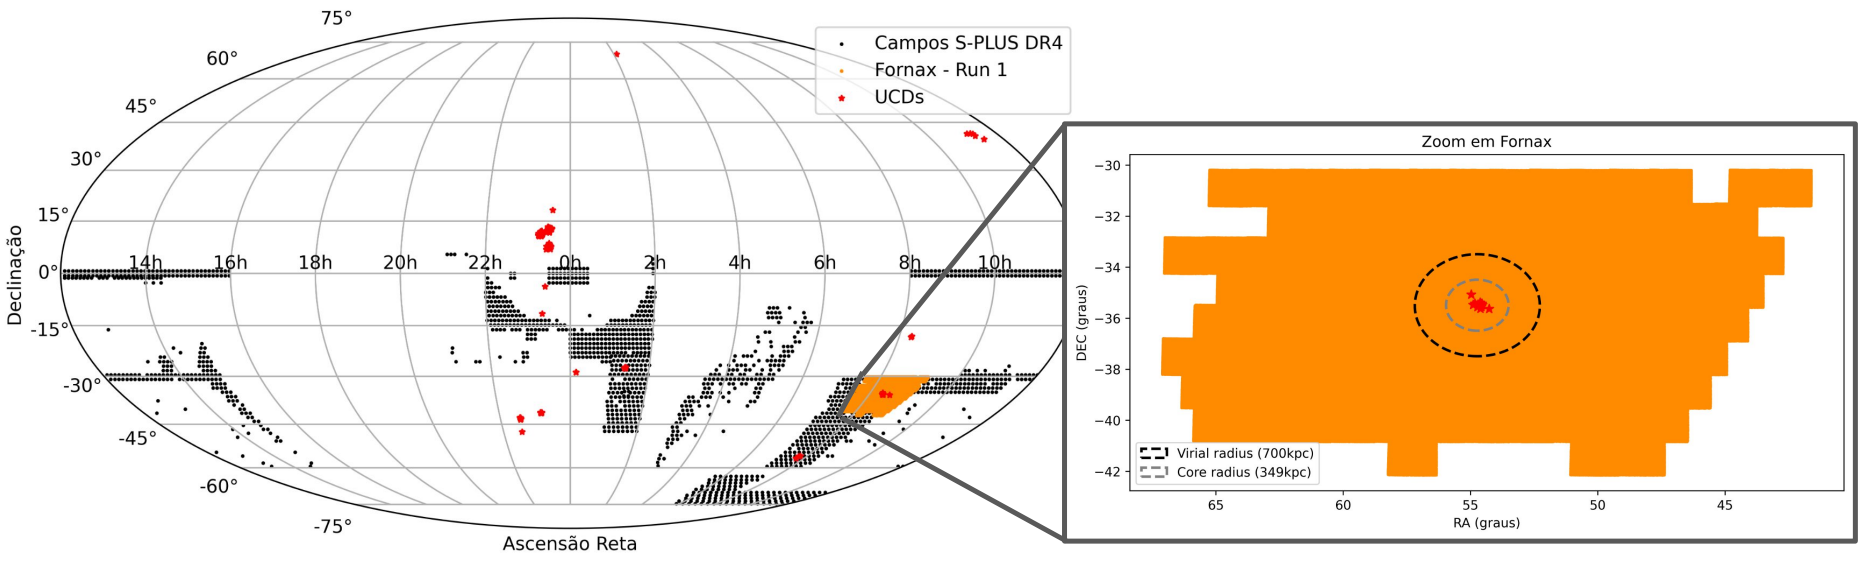
\includegraphics[width=1.\columnwidth,angle=0]{distribution_know_ucds.png}
    \caption[]{Distribuição dos campos observados do S-PLUS DR4 no céu em coordenadas equatoriais. Os pontos pretos representam os campos do S-PLUS DR4, enquanto os pontos azuis indicam as UCDs selecionadas como conhecidas vindas de \cite{catalog_ucds}. A área em laranja corresponde ao Aglomerado de Fornax com a redução da fotometria vinda de \cite{haack2024splusfornaxprojectsfp}, denominados \textit{Run 1}. As linhas de grade mostram a Ascensão Reta (em horas) e Declinação (em graus).}
    \label{distribution_know_ucds}
\end{figure}

Os objetos compilados presentes na nossa amostra de Fornax tiveram suas propriedades estudadas por \cite{Mieske_2008_2}, onde todos os alvos foram confirmados como pertencentes ao aglomerado por meio de pesquisas espectroscópicas (\citealt{Drinkwater_2000}, \citealt{Mieske_2002} \& \citeyear{Mieske_2004}, \citealt{Richtler_2004} \& \citeyear{Richtler_2008}). Dessas descobertas, as 5 primeiras UCDs (chamadas de UCDs clássicas) foram encontradas em Fornax, com a confirmação vinda de \cite{Drinkwater_2000}.

Dessas UCDs conhecidas, foi feito um cruzamento com os dados de Fornax utilizados neste trabalho. Obtivemos 16 objetos correspondentes na nossa amostra. Na Tabela \ref{ucds_fornax_propriedades}, apresentamos a lista dessas UCDs conhecidas e suas propriedades fornecidas por \citealt{Mieske_2008_2}.

\begin{table}[!ht]
    \centering
    \caption{Propriedades das UCDs identificadas na região de Fornax com dados da amostra deste estudo, fornecidas por \citealt{Mieske_2008_2}. As colunas representam: Nome - identificação do objeto; RA - Ascensão Reta em graus; Dec - Declinação em graus; Massa Total - massa total do objeto em $10^6 \, M_\odot$; $M/L$ - razão massa-luminosidade; [Fe/H] - metalicidade em dex; $r_h$ - raio de meia-luz em parsecs; $\sigma$ - dispersão de velocidade em km/s.}
    \begin{tabular}{lcccccccc}
        \toprule
        Nome & RA & Dec & Massa Total & $M/L$ & [Fe/H] & $r_h$ & $\sigma$ \\
        & (graus) & (graus) & ($10^6 \, M_\odot$) & & (dex) & (pc) & (km/s)\\
        \midrule
        UCD3, F-19 & 54.72542 & -35.55933 & $93.6 \pm 14.0$ & $4.69 \pm 0.70$ & -0.4 & 89.7 & 22.8 \\
        UCD1       & 54.26375 & -35.63461 & $32.1 \pm 3.9$  & $4.99 \pm 0.60$ & -0.7 & 22.4 & 27.1 \\
        F-24       & 54.89958 & -35.47350 & $24.5 \pm 7.8$  & $3.44 \pm 1.10$ & -0.4 & 29.5 & 21.4 \\
        UCD5       & 54.96908 & -35.07336 & $18.0 \pm 4.5$  & $3.37 \pm 0.85$ & -1.2 & 31.2 & 18.7 \\
        F-1a       & 54.52625 & -35.48300 & $16.2 \pm 3.8$  & $2.45 \pm 0.58$ & 0.0  & 23.1 & 18.7 \\
        F-9        & 54.60625 & -35.62853 & $14.1 \pm 3.6$  & $4.72 \pm 1.20$ & -0.8 & 9.1  & 25.7 \\
        F-5        & 54.54500 & -35.42950 & $13.7 \pm 2.4$  & $3.16 \pm 0.55$ & -0.3 & 5.0  & 34.5 \\
        F-6        & 54.56875 & -35.43878 & $12.5 \pm 2.4$  & $5.32 \pm 1.00$ & 0.2  & 7.3  & 27.3 \\
        F-7        & 54.57333 & -35.55067 & $10.5 \pm 1.4$  & $4.21 \pm 0.57$ & -1.3 & 14.9 & 20.1 \\
        F-12       & 54.62083 & -35.38231 & $8.3 \pm 2.9$   & $2.36 \pm 0.83$ & -0.4 & 10.3 & 22.9 \\
        F-11       & 54.61792 & -35.42736 & $5.7 \pm 3.7$   & $1.64 \pm 1.10$ & -0.9 & 3.6  & 26.2 \\
        F-34       & 54.55292 & -35.48250 & $5.5 \pm 1.3$   & $3.17 \pm 0.74$ & -0.9 & 4.0  & 24.6 \\
        F-22       & 54.82375 & -35.42503 & $5.3 \pm 1.0$   & $2.13 \pm 0.39$ & -0.4 & 10.0 & 22.8 \\
        F-53       & 54.66917 & -35.48611 & $3.9 \pm 1.0$   & $2.66 \pm 0.69$ & -0.9 & 4.4  & 19.6 \\
        F-51       & 54.57125 & -35.44203 & $3.5 \pm 0.9$   & $2.38 \pm 0.62$ & -0.8 & 4.2  & 20.1 \\
        F-59       & 54.70375 & -35.46225 & $1.3 \pm 0.6$   & $0.94 \pm 0.43$ & -2.1 & 5.7  & 9.8  \\
        \bottomrule
    \end{tabular}
    \label{ucds_fornax_propriedades}
\end{table}

Fazendo um cruzamento das UCDs conhecidas do catálogo de \cite{catalog_ucds} com os dados da fotometria original do S-PLUS DR4, obtivemos 9 objetos, em comparação com os 16 que obtivemos anteriormente. Isso ressalta a importância da redução da fotometria de Fornax vinda de \cite{haack2024splusfornaxprojectsfp} para a identificação das nossas galáxias de interesse.

Fazendo um cruzamento dessas UCDs conhecidas nos nossos dados com o catálogo GAIA DR3 \citep{GAIA_DR3}, que fornece informações de classificação estrela-galáxia-quasar, observamos que das 16, 8 têm probabilidade maior que 50\% de serem galáxias e 8 têm probabilidade maior que 50\% de serem estrelas. Esse fato mostra a dificuldade de parte da classificação desses objetos. Mostramos na Tabela \ref{tab_ucds_stars_galaxy_like} as médias e desvios padrões das magnitudes dos dados usados desses dois grupos.

\begin{table}[!ht]
    \centering
    \caption{Comparação das 12 magnitudes do S-PLUS DR4 (Run 1) da abertura APER\_6 corrigidas pela extinção entre as UCDs conhecidas, separadas em dois grupos: classificação estrela (PSS > 0,5) ou galáxia (PGal > 0,5) pelo Gaia DR3.}   
    \begin{tabular}{lcccc}
        \toprule
        Filtro & \multicolumn{2}{c}{UCD(PGal>0,5)} & \multicolumn{2}{c}{UCD(PSS>0,5)} \\
        & Média & $\sigma$ & Média & $\sigma$ \\
        \midrule
        u & 21,73 & 0,83 & 22,03 & 0,37 \\
        J0378 & 21,13 & 0,84 & 22,04 & 0,49 \\
        J0395 & 21,29 & 1,04 & 22,42 & 1,23 \\
        J0410 & 20,41 & 0,53 & 21,63 & 0,57 \\
        J0430 & 20,29 & 0,67 & 21,16 & 0,33 \\
        g    & 19,88 & 0,73 & 21,07 & 0,63 \\
        J0515 & 19,60 & 0,63 & 20,75 & 0,46 \\
        r    & 18,08 & 0,67 & 20,41 & 0,36 \\
        J0660 & 19,00 & 0,68 & 20,27 & 0,39 \\
        i    & 18,75 & 0,72 & 20,10 & 0,44 \\
        J861 & 18,58 & 0,69 & 19,82 & 0,36 \\
        z    & 18,54 & 0,72 & 19,98 & 0,51 \\
        \bottomrule
    \end{tabular}
    \label{tab_ucds_stars_galaxy_like}
\end{table}

Concluímos pela Tabela \ref{tab_ucds_stars_galaxy_like} que o grupo de UCDs classificadas como galáxias pelo GAIA DR3 é mais brilhante que o grupo classificado como estrelas. Observando ainda a banda fotométrica $r$, usada como referência devido à sua profundidade e qualidade, temos as UCDs classificadas como galáxias no intervalo de 17,64 a 19,83 magnitudes, enquanto as classificadas como estrelas estão no intervalo de 19,8 a 20,83 magnitudes. Podemos usar estes intervalos como referência para a seleção dos objetos de interesse.

Pelas propriedades da Tabela \ref{ucds_fornax_propriedades}, mostramos na Figura \ref{r_h_M_ucds} a relação entre a massa e o raio de meia-luz das UCDs conhecidas de Fornax. Observamos uma conclusão similar: o grupo de UCDs classificadas como galáxias pelo GAIA DR3 é mais brilhante que o grupo classificado como estrelas, e assim, tem uma relação entre a massa e o raio de meia-luz maior.

\begin{figure}[!ht]
    \centering
    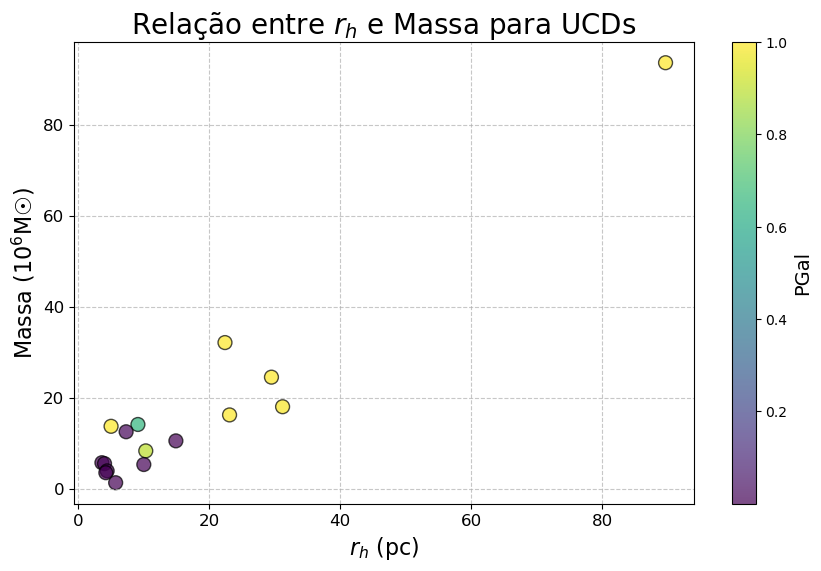
\includegraphics[width=0.8\columnwidth,angle=0]{r_h_M_ucds.png} 
    \caption[]{Relação entre a massa e o raio de meia-luz das UCDs conhecidas de Fornax. Barra de cor pela classificação como galáxia (PGal) vinda do Gaia DR3.}
    \label{r_h_M_ucds}
\end{figure}

Na Figura \ref{distribuicao_fwhm_image_r_r_aper6_ucds_fornax}, mostramos a distribuição de \textit{FWHM (r-band)} em função da banda \textit{r\_APER\_6} para UCDs de Fornax, coloridas pelo classificador de galáxia (PGal) do Gaia DR3. Percebemos que, para os objetos mais fracos, o classificador do Gaia erra mais ao classificá-los, atribuindo maiores probabilidades de serem estrelas.

\begin{figure}[!ht]
    \centering
    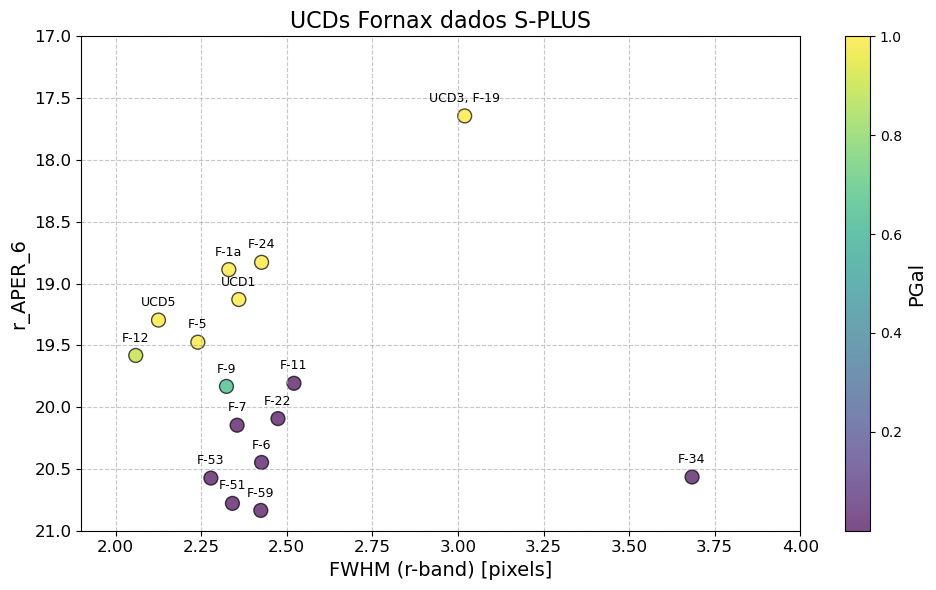
\includegraphics[width=0.8\columnwidth,angle=0]{distribuicao_fwhm_image_r_r_aper6_ucds_fornax.png}
    \caption[]{Distribuição de \textit{FWHM (r-band)} em função da magnitude \textit{r\_APER\_6} para UCDs de Fornax nos dados do S-PLUS.}
    \label{distribuicao_fwhm_image_r_r_aper6_ucds_fornax}
\end{figure}


\subsection*{Distribuição UCDs em Fornax}
Na Figura \ref{distribuicao_ucds_center}, apresentamos a distribuição de UCDs conhecidas nos dados do S-PLUS, com ênfase no centro do aglomerado.

\begin{figure}[!ht]
    \begin{center}
    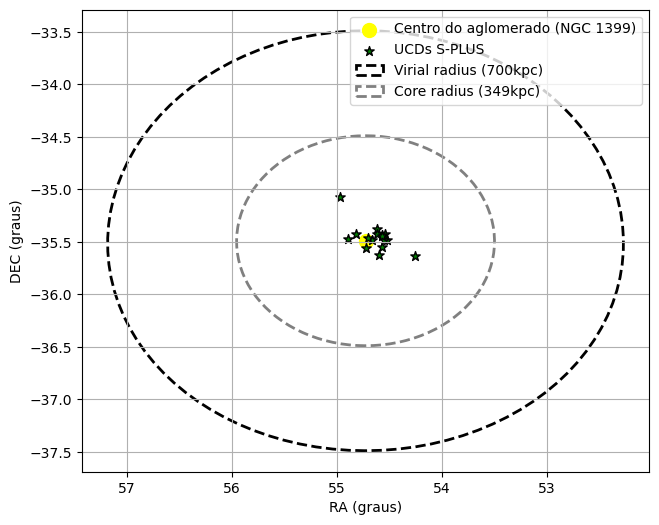
\includegraphics[width=1.\columnwidth,angle=0]{distribuicao_ucds_center.png}
    \caption[]{Distribuição das UCDs conhecidas de Fornax nos dados do S-PLUS. Os pontos azuis representam as UCDs conhecidas, coloridas pelo raio de virial (virial radius) e o raio do núcleo (core radius).}
    \label{distribuicao_ucds_center}
    \end{center}
\end{figure}

Nesta figura, apresentamos a distribuição das UCDs nos dados do S-PLUS, destacando o raio de virial ($virial \, radius$) e o raio do núcleo ($core \, radius$). Utilizamos o $virial \, radius$ como 700 kpc \citep{Drinkwater_2001} e definimos o $core \, radius$ como aproximadamente 349 kpc, o que corresponde a 1 grau no céu (aproximadamente metade do raio de virial). Essa representação evidencia que os objetos estão ainda mais concentrados no centro do aglomerado.

Para a conversão de kpc para graus, usamos a relação:

\begin{equation}
    \theta = \frac{d}{D} \times \frac{180}{\pi}
\end{equation}
onde $d$ é o tamanho em kpc, $D$ é a distância em kpc até o objeto, e $\theta$ é o tamanho em graus. Considerando que Fornax está a aproximadamente $20 \, \text{Mpc}$ \citep{Blakeslee_2009}, o que corresponde a um módulo de distância de $31.51 \, \text{mag}$, nessa distância, 1 grau equivale a $0.349 \, \text{Mpc}$. Assim, para as propriedades de Fornax, adotamos os valores apresentados na Tabela \ref{tab:properties_fornax}.

\begin{table}[!ht]
    \centering
    \caption{Propriedades do aglomerado de Fornax. Referências usadas (\citealp{Drinkwater_2001}, \citealp{Blakeslee_2009}), \citealp{Maddox_2019}).}   
    \begin{tabular}{lc}
        \toprule
        % &  \\
        \midrule
        Massa ($M_\odot$) & $7\pm 2. 10^{13}$ \\
        Virial Radius (Mpc) & 0.7 \\
        Virial Radius (graus) & 2 \\
        Core Radius (Mpc) & 0.349 \\
        Core Radius (graus) & 1 \\
        Dispersão de velocidade ($km s^{-1}$) & 318 \\
        Modulo de distância (mag) & 31.51 \\
        \bottomrule
    \end{tabular}
    \label{tab:properties_fornax}
\end{table}

Na Figura \ref{distribuicao_ucds_center}, observamos que as UCDs conhecidas estão concentradas no centro do aglomerado. A presença de UCDs no centro é consistente com outros estudos, que também identificaram essas estruturas em regiões de alta densidade de galáxias massivas. No entanto, esse padrão pode estar relacionado ao viés das pesquisas espectroscópicas, que tendem a se concentrar nas áreas centrais do aglomerado, e não necessariamente reflete a distribuição real das UCDs em Fornax.

\section{Seleção Galáxias Massivas em Fornax}\label{subsec:galaxias_massivas}
Para mostrar a distribuição espacial dos objetos em Fornax, também é útil apresentar as regiões com a presença das principais galáxias massivas encontradas. 

A presença e a distribuição das galáxias massivas são importantes, pois, além do centro do aglomerado, onde as UCDs estão mais concentradas, as galáxias massivas também podem desempenhar um papel relevante na localização dessas estruturas. Segundo o cenário de {\it tidal stripping}, as UCDs podem ser formadas a partir da interação com uma galáxia mais massiva. Assim, quando uma galáxia anã nucleada começa a interagir com uma galáxia mais massiva, após algumas passagens orbitais, parte de sua matéria pode ser removida, resultando no núcleo remanescente, que observamos como sendo uma UCD. Mostramos então também onde as principais galáxias massivas estão localizadas no aglomerado, e como a distribuição das candidatas a UCDs se compara com a distribuição dessas galáxias.

Selecionamos os trabalhos provenientes de uma lista de referências das galáxias confirmadas do aglomerado (\citealp{Ferguson_1989}, \citealp{Jordan_2007}, \citealp{Venhola_2018}). A partir dessas listas de objetos, filtramos utilizando o catálogo de \cite{Lima_2024}, que compila redshifts espectroscópicos confirmados. Selecionamos apenas os objetos com valores presentes e dentro da faixa de redshift do aglomerado de Fornax. Para identificar as galáxias mais massivas entre esses objetos, realizamos um corte na magnitude absoluta $M_r$. Calculamos a magnitude absoluta utilizando o módulo de distância da Tabela \ref{tab:properties_fornax} e a magnitude aparente $m_r$ dos objetos.

Utilizando todos os objetos da nossa amostra de Fornax com redshift confirmado nesse mesmo intervalo, mostramos na Figura \ref{hist_mag_abs} a distribuição da magnitude absoluta $M_r$ dos objetos.

\begin{figure}[!ht]
    \centering
    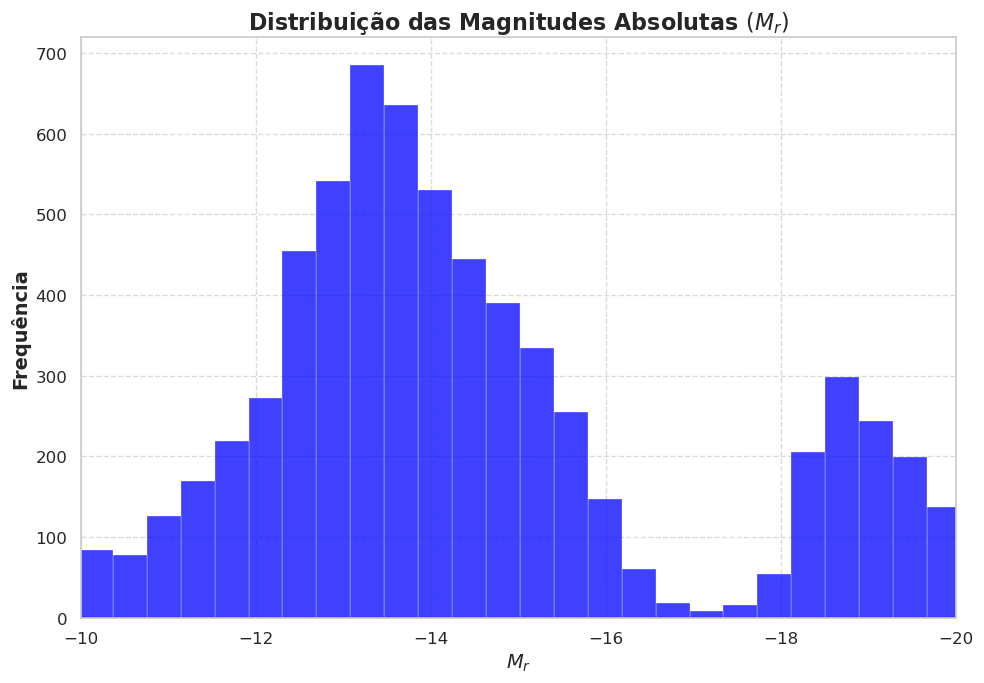
\includegraphics[width=0.7\columnwidth,angle=0]{hist_mag_abs.png}
    \caption[]{Distribuição da magnitude absoluta $M_r$ dos objetos com redshift confirmado na região de Fornax.}
    \label{hist_mag_abs}
\end{figure}

Observamos dois picos de magnitudes, um em torno de -13 e outro em torno de -19. Para o regime das galáxias mais massivas, e assim mais brilhantes, selecionaremos, assim como adotado em \cite{Saifollahi_2021}, um corte em $M_r \leq -18$ para a seleção das galáxias massivas, onde estaremos considerando esse segundo pico de magnitudes.


Na Figura \ref{distribuicao_galaxias_massivas}, apresentamos a distribuição espacial das galáxias massivas em Fornax. Acrescentameo em cada uma delas um raio de 200

\begin{figure}[!ht]
    \centering
    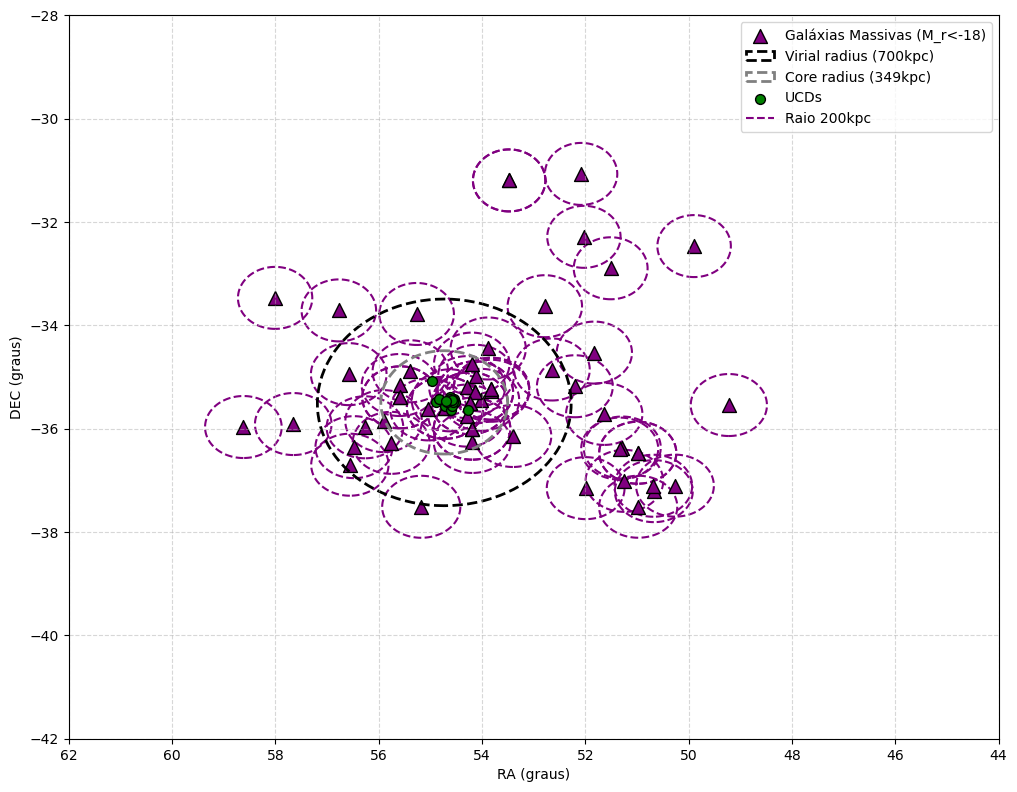
\includegraphics[width=1.\columnwidth,angle=0]{distribuicao_galaxias_massivas.png}
    \caption[]{Distribuição das galáxias massivas em Fornax nos dados do S-PLUS. Os pontos roxo representam as galáxias massivas, coloridas pelo raio de virial (virial radius) e o raio do núcleo (core radius).}
    \label{distribuicao_galaxias_massivas}
\end{figure}




\section{Aprendizado de Máquina}\label{sec:aprendizado_maquina}

Neste trabalho, utilizamos aprendizado de máquina para auxiliar na identificação de candidatas a galáxias ultracompactas (UCDs) no aglomerado de Fornax, com base em dados fotométricos do S-PLUS. A distinção entre UCDs e outros objetos compactos, como estrelas, é desafiadora. Para abordar essa dificuldade, empregamos um método supervisionado que classifica os objetos em duas categorias principais: compactos e extensos. Essa abordagem permite identificar objetos compactos com características fotométricas semelhantes às de galáxias, facilitando a seleção de candidatas a UCDs.

O processo envolve o treinamento de um modelo de classificação com um conjunto de dados rotulados, onde as classes (compactos e extensos) são definidas com base em parâmetros fotométricos, como a largura à meia altura (\textit{FWHM}) e magnitudes em diferentes bandas. Após o treinamento, o modelo é aplicado a um conjunto maior de dados para prever a classe de novos objetos, permitindo a seleção de candidatos para análise detalhada.

Esse método conscinte então na idiea de que, no conjunto de dados de treinamento, os objetos compactos são predominantemente estrelas, enquanto os objetos extensos são principalmente galáxias. Assim, é esperado que algumas classificações sejam feitas de forma errada, e é nessa proposta que o modelo foi treinado: encontrar aqueles com maior probabilidade de serem extensos, mas que fazem parte do conjunto dos compactos.

Nas subseções seguintes, apresentamos a construção da amostra de treino, o tratamento de valores faltantes, o treinamento do modelo e a avaliação do desempenho do classificador.

\subsection{Amostra de treino}\label{subsec:amostra_treino}
Para a amostra de treino, é desejável implementar uma estratégia que auxilie na identificação de candidatas a UCDs. Uma abordagem comum é a utilização de um classificador, onde um modelo é treinado com um conjunto de dados rotulados e, posteriormente, é capaz de classificar novos objetos com base nas características aprendidas durante o treinamento.

Um exemplo semelhante é o problema de classificação de quasares, que são fontes pontuais facilmente confundidas com estrelas, mas possuem características que os distinguem destas. Nesse caso, um modelo de classificação pode ser treinado com dados de quasares e estrelas, realizando a separação entre eles. No entanto, para UCDs, temos uma quantidade limitada de objetos conhecidos, impossibilitando um conjunto de dados grande o suficiente para treinar um modelo de classificação direta de UCDs.

A proposta deste trabalho é utilizar um modelo de classificação indireta, onde treinamos um modelo para classificar objetos em duas classes: objetos compactos e objetos extensos e selecionar os objetos compactos com fotometria consistente com a dos objetos extensos (galáxias). Um dos parâmetros disponíveis para os objetos da amostra é a largura à meia altura, full width at half maximum (\textit{FWHM}). O \textit{FWHM} representa a largura do perfil de intensidade de uma fonte de luz na metade de sua intensidade máxima. Em nosso estudo, essa métrica é particularmente relevante, pois ao lidar com estrelas e UCDs, ela auxilia na identificação de fontes pontuais. Para cada uma das 12 bandas fotométricas, temos a \textit{FWHM} disponível associada.

Usamos a \textit{FWHM} normalizada para cada uma das bandas. O valor normalizado é dado pela \textit{FWHM} do objeto dividido pela \textit{FWHM} do campo. A normalização é feita para garantir que a largura do perfil de intensidade seja independente da qualidade da imagem e da região observada, quando comparada entre objetos de diferentes campos.

As estrelas, por sua natureza, são fontes pontuais; por isso, esperamos que a \textit{FWHM} desses objetos seja menor do que a de objetos extensos, como as galáxias, exceto, claro, para galáxias ultra compactas.

Realizamos um cruzamento de dados de treinamento com o catálogo GAIA DR3 \citep{GAIA_DR3}, que fornece informações de classificação estrela-galáxia-quasar. Com esses dados, selecionamos um subconjunto de objetos com as probabilidades de serem estrelas e galáxias maiores que 90\%. A partir desse subconjunto, analisamos a distribuição dos valores de \textit{FWHM} para estrelas e galáxias em cada banda fotométrica.

Na Figura \ref{distribution_of_stars_and_galaxies}, temos um histograma da distribuição de \textit{FWHM} para estrelas e galáxias na banda $r$, sendo ela a banda com a melhor separação entre as duas classes.

\begin{center}
    \begin{minipage}{0.45\textwidth}
        \centering
        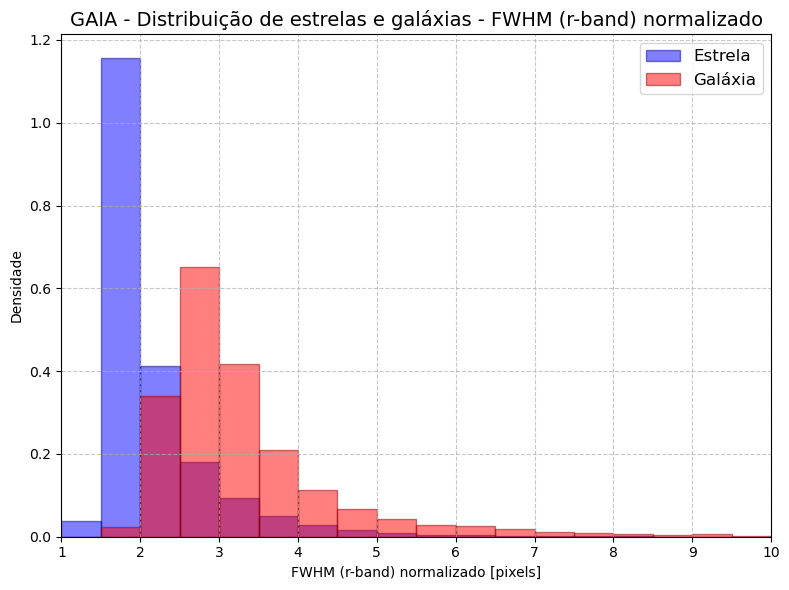
\includegraphics[width=\linewidth]{distribution_of_stars_and_galaxies.png}
        \captionsetup{}
        \captionof{figure}{Histograma da distribuição de \textit{FWHM (r-band) normalizado} dos objetos do cruzamento do S-PLUS DR4 de Fornax, com o catálogo GAIA DR3 com a classificação para estrelas e galáxias com probabilidade maior que 90\%.}
        \label{distribution_of_stars_and_galaxies}
    \end{minipage}
    \hfill
    \begin{minipage}{0.45\textwidth}
        \centering
        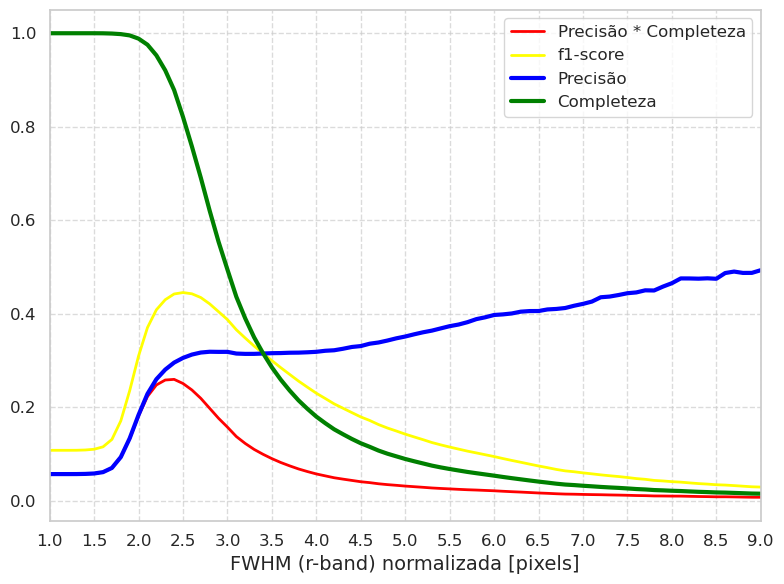
\includegraphics[width=\linewidth]{purity_completeness.png}
        \captionsetup{}
        \captionof{figure}{Relação entre Pureza e Completeza para diferentes cortes de \textit{FWHM}. O ponto ideal é aquele que maximiza o produto entre as duas variáveis, indicando o corte que melhor separa as duas classes.}
        \label{purity_completeness}
    \end{minipage}
\end{center}

Há uma diferença entre os picos das distribuições de \textit{FWHM} para estrelas e galáxias. Portanto, o objetivo é definir um corte na \textit{FWHM} para selecionar dois conjuntos: um contendo objetos compactos e outro contendo objetos extensos. No conjunto de objetos compactos, predominam as estrelas, enquanto no conjunto de objetos extensos, as galáxias são mais representativas.

A hipótese é que o modelo aprenda a distinguir as propriedades fotométricas de estrelas e galáxias independentemente da morfologia (ou FWHM) do objeto; numa segunda etapa, procuramos entre os objetos com morfologia estelar aqueles cuja fotometria indica que têm alta probabilidade de serem galáxias.

Para identificar, na Figura \ref{distribution_of_stars_and_galaxies}, a melhor divisão entre as duas classes, estabelecemos alguns cortes visando encontrar aquele que melhor separa cada população, minimizando a contaminação entre as duas populações. Para cada corte, definimos duas variáveis: Pureza e Completeza, ambas com respeito às galáxias. A Pureza representa a fração de galáxias após o corte em relação ao total de objetos restantes no corte final, fornecendo uma medida da pureza das galáxias no subconjunto. A Pureza é uma métrica que indica a proporção de galáxias corretamente identificadas em relação ao total de objetos classificados como galáxias. Ela também é conhecida como precisão, sendo sua definição dada na equação \ref{eq:precisao}.

Por outro lado, a Completeza representa a fração de galáxias após o corte em relação ao número total de galáxias que existiam, fornecendo uma estimativa de quantas galáxias são perdidas durante a seleção. Ela é definida na equação \ref{eq:completeza}.

A Figura \ref{purity_completeness} ilustra o produto entre Pureza e Completeza para diferentes valores de corte de \textit{FWHM}. O ponto ótimo que adotamos é aquele que maximiza o produto dessas duas variáveis, representando o corte que proporciona a melhor separação entre as duas classes.

O valor máximo de aproximadamente $0,12$ do produto entre pureza e completeza, selecionado para o corte, corresponde a um \textit{FWHM (r-band)} de 2,5 pixels. Esse corte representa o ponto de maximização para a separação das classes, com as galáxias associadas à classe de objetos extensos. No entanto, após alguns testes, decidimos realizar um corte para objetos compactos com \textit{FWHM} menores que 2 pixels, o que apresentou melhores resultados nos classificadores iniciais testados. Assim, para a amostra de treino, os objetos com \textit{FWHM (r-band)} menores que 2 pixels são considerados compactos, enquanto os objetos com \textit{FWHM (r-band)} maiores que 2,5 pixels são considerados extensos. Os demais cortes para a seleção de objetos compactos e extensos são descritos na subseção \ref{subsec:cuts}.

Os objetos com valores de \textit{FWHM} entre 2 e 2,5 pixels são considerados de transição, ou seja, não são classificados como compactos nem extensos para a amostra de treino devido à incerteza na classificação. No entanto, esses dados ainda serão utilizados na busca por candidatas a UCDs, aplicando o modelo treinado. Assim, esses objetos de transição não são incluídos no treinamento do modelo, mas permanecem na amostra de análise.

Na Figura \ref{amostra_treino}, temos a magnitude \textit{g\_APER\_6} em função da \textit{FWHM (r-band)} para a divisão entre as duas classes adotadas.

\begin{figure}[!ht]
    \centering
    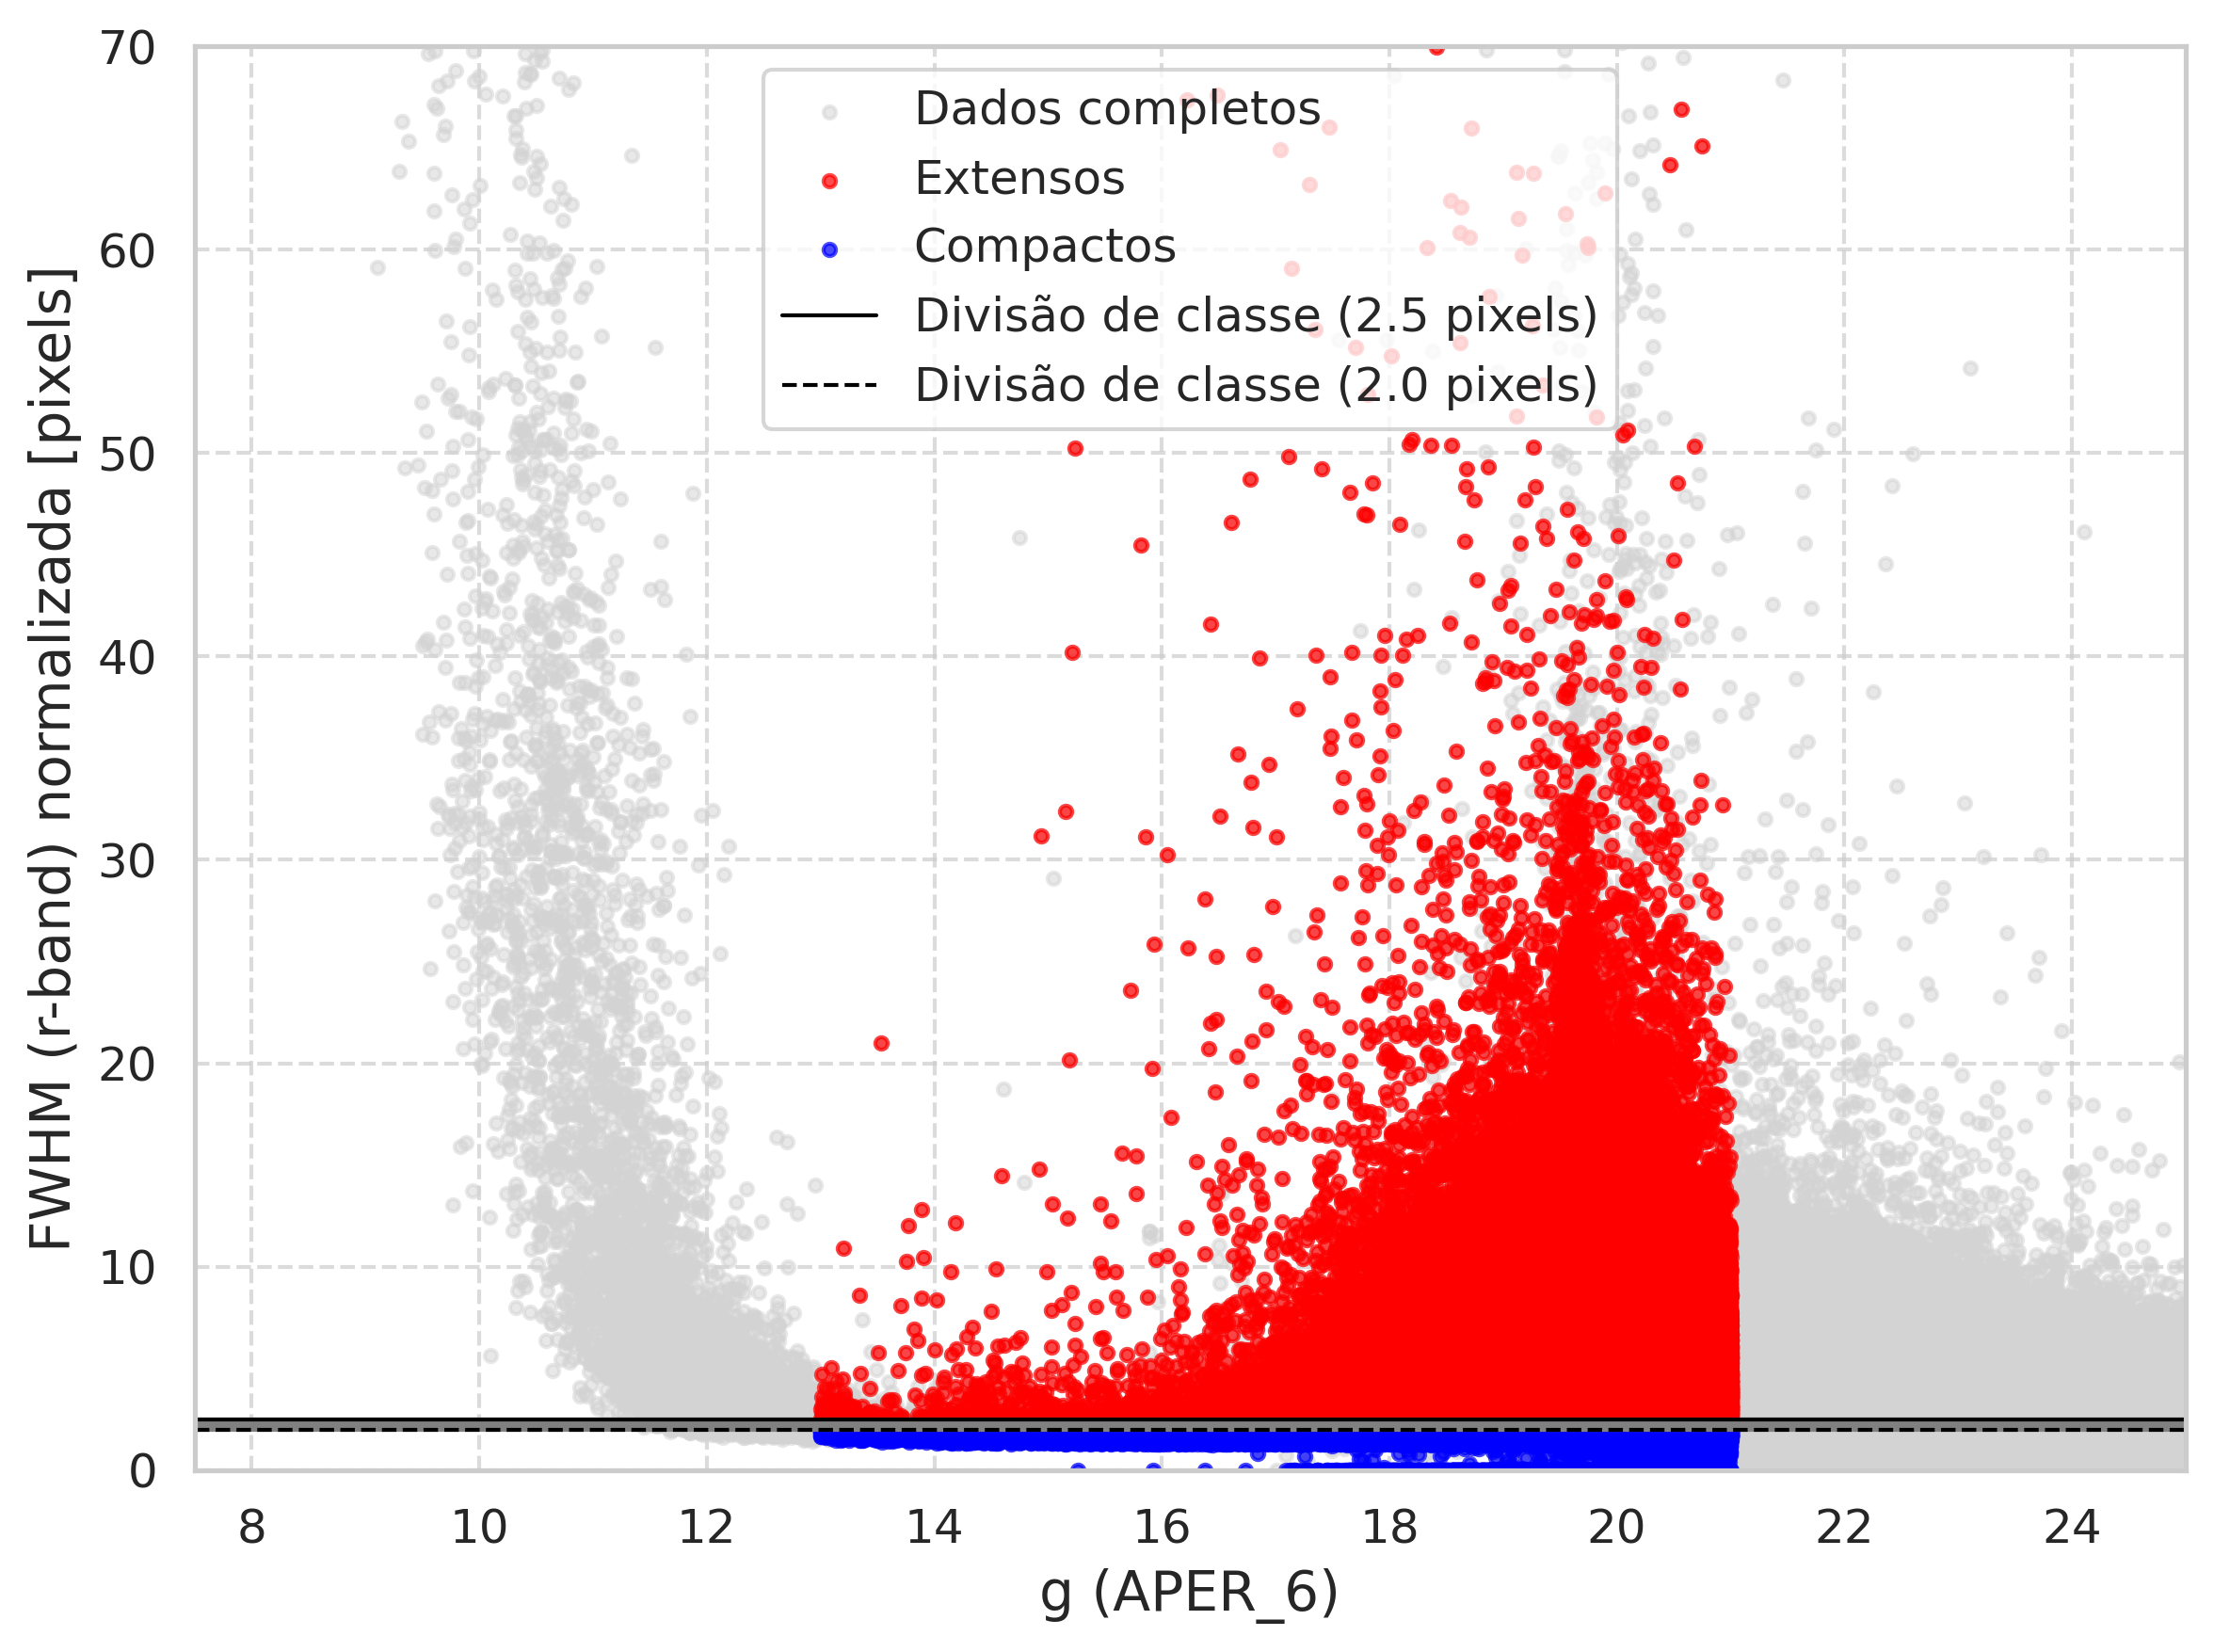
\includegraphics[width=0.85\columnwidth,angle=0]{amostra_treino.png}
    \caption[]{Distribuição da Largura Total na Metade Máxima (\textit{FWHM} r-band) em função da magnitude \textit{g\_APER\_6} para objetos na região de Fornax, usando dados do S-PLUS Data Release 4. Objetos compactos são representados por pontos azuis, enquanto objetos extensos são indicados por pontos vermelhos. Os dados totais são mostrados em cinza. Divisão das classes: compactos (\textit{FWHM}$\leq$2 pixels) e extensos (\textit{FWHM}$\geq$2.5 pixels). Os dados entre 2 e 2.5 pixels não são usados para o treinamento do modelo, mas são mantidos na amostra de análise.}
    \label{amostra_treino}
\end{figure}

\subsection{Valores faltantes na amostra de treino}\label{subsec:valores_faltantes}
Ao preparar os dados para treinar modelos com medições do S-PLUS, decidimos alterar os valores das magnitudes na abertura APER\_6 acima de 30 para \texttt{NaN} (Not a Number). Essa decisão foi tomada para evitar que objetos com medições de baixa qualidade influenciassem o treinamento do modelo.

Na Figura \ref{missing_values_hist} temos um gráfico da fração de dados disponíveis para cada uma das bandas fotométricas.

\begin{figure}[!ht]
    \begin{center}
    % \setcaptionmargin{1cm}
    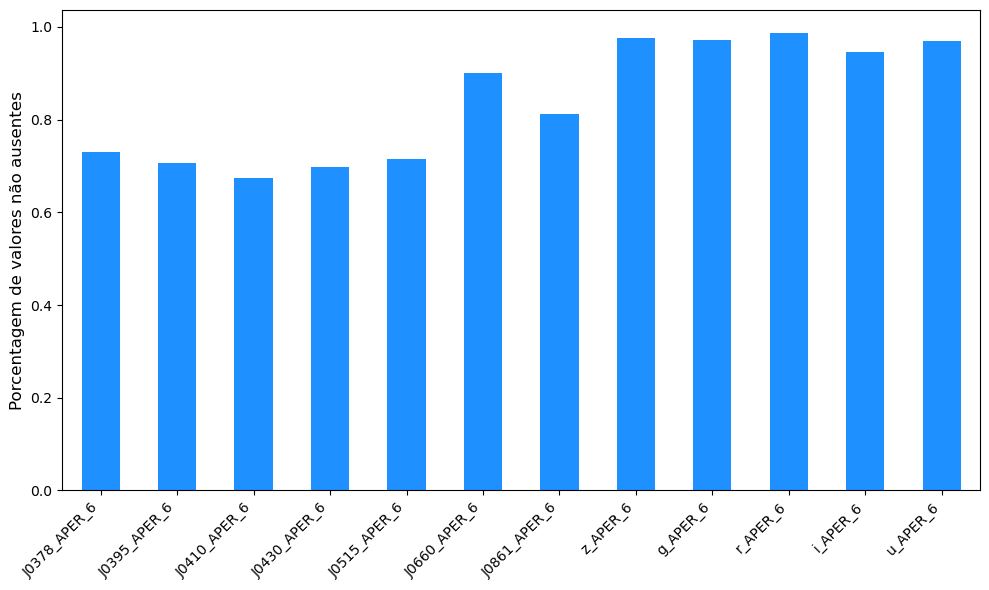
\includegraphics[width=0.8\columnwidth,angle=0]{missing_values_hist.png}
    \caption[]{Fotometria disponível em cada banda fotométrica. Cada barra representa a fração de objetos com valores disponíveis para a respectiva banda.}
    \label{missing_values_hist}
    \end{center}
\end{figure}

O gráfico mostra que a quantidade de dados ausentes varia consideravelmente entre as diferentes bandas fotométricas. A banda $u$, juntamente com algumas bandas estreitas no azul, como $J0378$, $J0395$, $J0410$ e $J0430$, apresentam a maior quantidade de valores faltantes, o que pode prejudicar a análise.

Mostramos na Figura \ref{msno_matriz} uma visualização da distribuição dos dados faltantes, onde cada linha representa um objeto e cada coluna uma banda fotométrica. As células em branco indicam valores faltantes. A Figura \ref{msno_matriz_ord} mostra a mesma matriz, mas ordenada pela primeira coluna de atributos. Ordenamos a matriz para identificar padrões de valores faltantes que possam ser úteis para a imputação dos dados.

\begin{center}
    \begin{minipage}{0.45\textwidth}
        \centering
        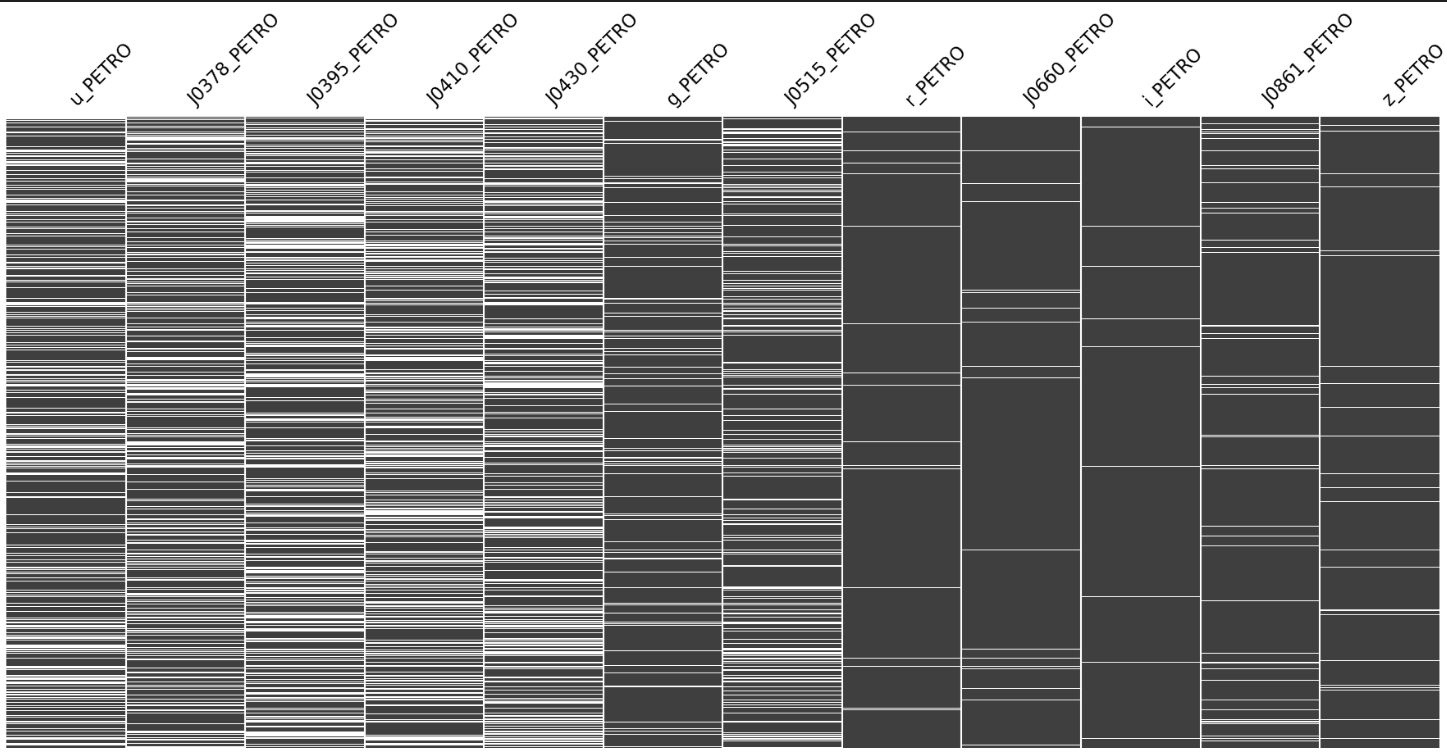
\includegraphics[width=\linewidth]{msno_matriz.png}
        \captionsetup{}
        \captionof{figure}{Distribuição de valores em cada banda fotométrica. Cada barra vertical representa as linhas da tabela original. As linhas em preto indicam objetos com valores disponíveis para a respectiva banda, enquanto os espaços em branco correspondem a linhas na tabela sem valores medidos.}
        \label{msno_matriz}
    \end{minipage}
    \hfill
    \begin{minipage}{0.45\textwidth}
        \centering
        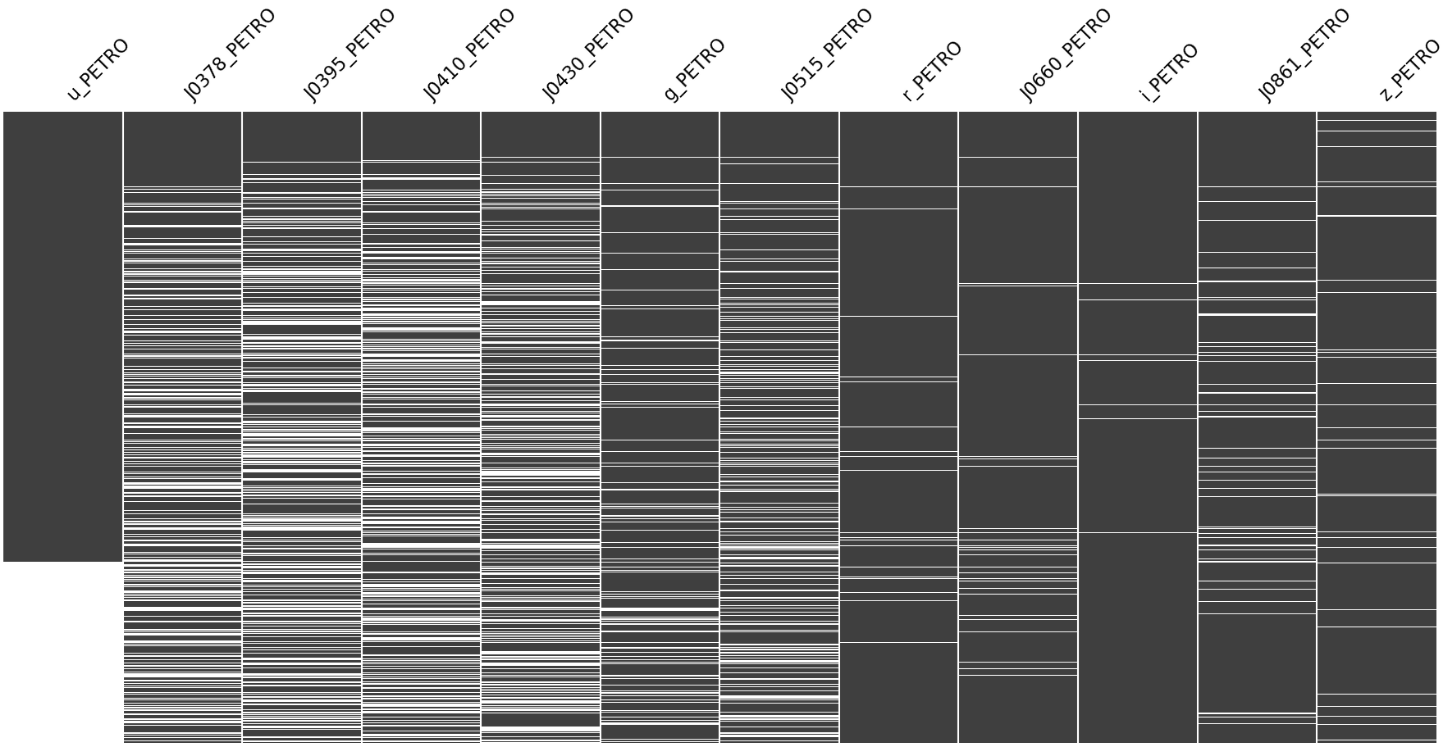
\includegraphics[width=\linewidth]{msno_matriz_ord.png}
        \captionsetup{}
        \captionof{figure}{Distribuição de valores em cada banda fotométrica, ordenada de forma que os valores disponíveis na última coluna de atributos sejam agrupados no início (coluna preenchida), enquanto os valores faltantes sejam posicionados ao final.}
        \label{msno_matriz_ord}
    \end{minipage}
\end{center}

Uma maneira melhor de visualizar se esses valores ausentes têm alguma correlação é mostrada na Figura \ref{matriz_correlacao}, que apresenta a matriz de correlação entre os valores faltantes. Valores próximos de 1 ou -1 indicam que os valores faltantes estão, respectivamente, positivamente ou negativamente correlacionados. Valores próximos de 0 indicam que os valores faltantes são independentes.

\begin{figure}[!ht]
    \begin{center}
    % \setcaptionmargin{1cm}
    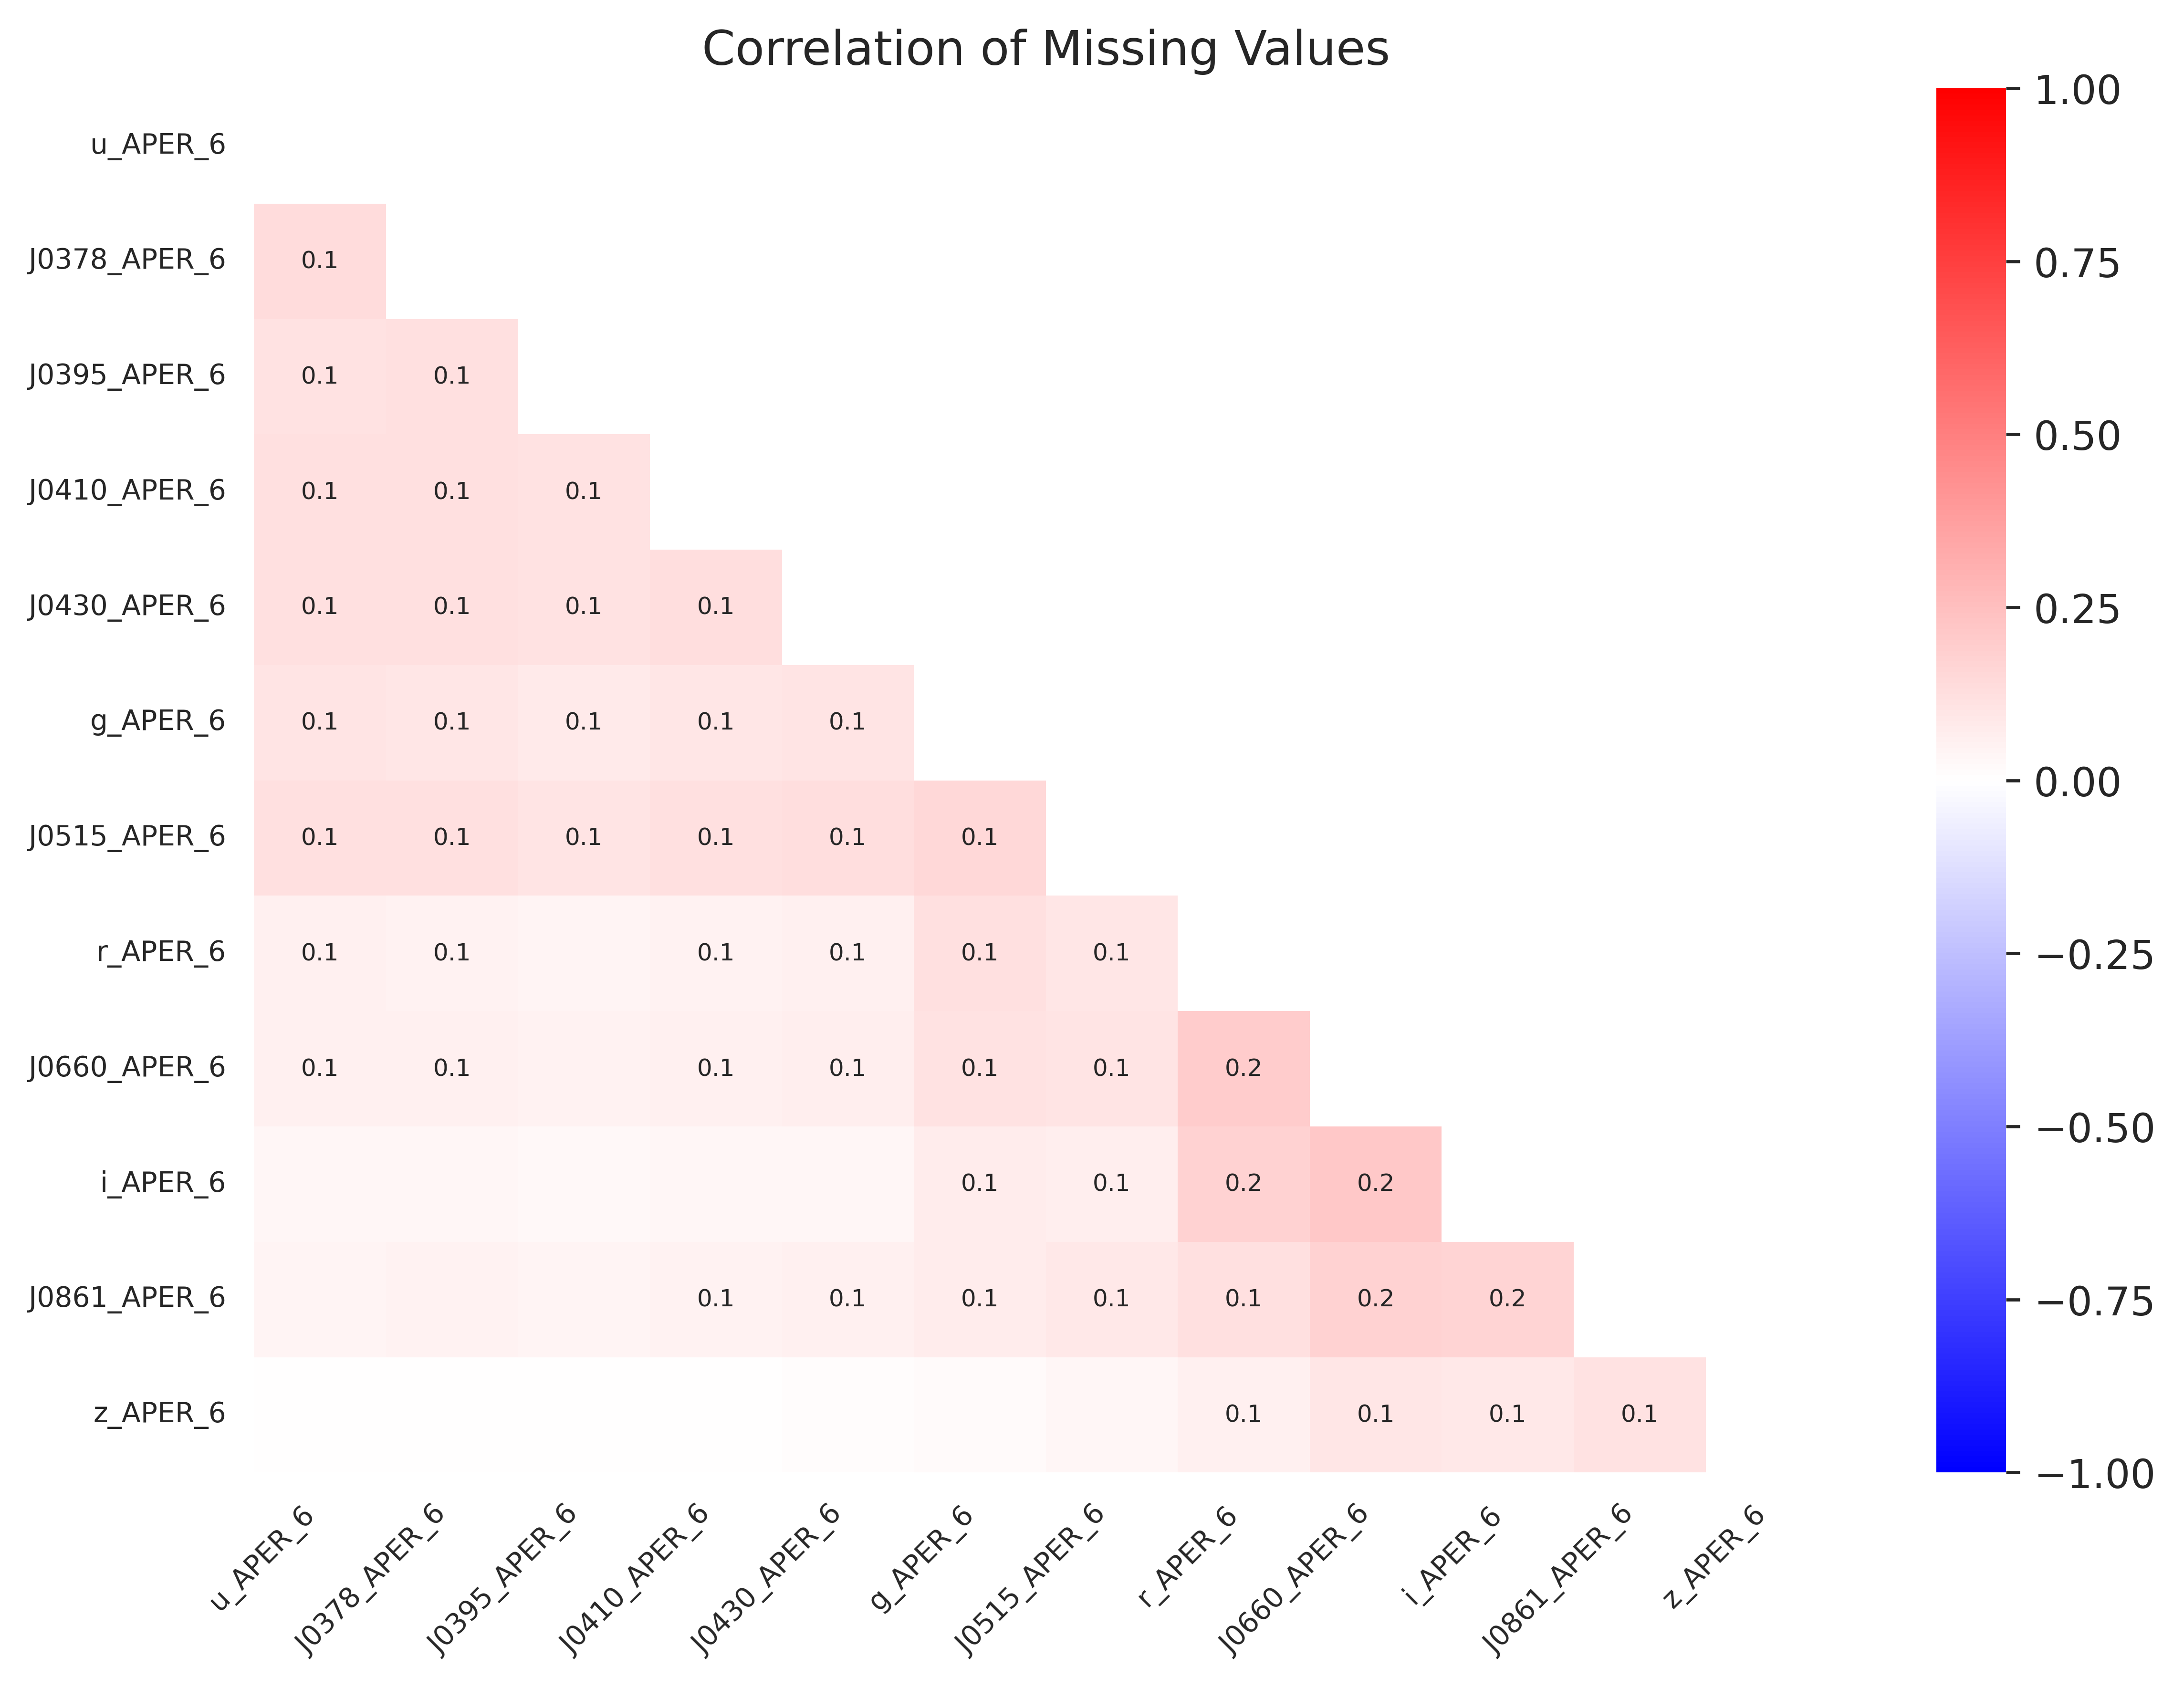
\includegraphics[width=0.85\columnwidth,angle=0]{matriz_correlacao.png}
    \caption[]{Matriz de correlação entre os valores faltantes. Cada célula contém o coeficiente de correlação entre os valores faltantes de duas bandas fotométricas.}
    \label{matriz_correlacao}
    \end{center}
\end{figure}

Pela Figura \ref{matriz_correlacao}, observamos que a maioria dos valores faltantes não apresenta correlação significativa, sugerindo que os dados faltantes são independentes.

Existem várias técnicas para lidar com esses valores ausentes. Uma maneira simples e comum é remover os objetos que possuem algum dado faltante, mas isso pode gerar uma perda de informação para o treinamento. Outra alternativa é substituir os valores faltantes pela média dos valores restantes, mas isso pode introduzir um viés na nossa seleção. Há ainda a opção de utilizar algum valor padrão, como \texttt{NaN} (Not a Number) ou -1, porém, essa estratégia pode acabar confundindo o classificador, principalmente se esses valores não tiverem um significado claro para o modelo.

A técnica que adotamos para lidar com os valores faltantes foi a imputação dos dados utilizando o Método de Imputação Múltipla por Equações Encadeadas (MICE) (\citealp{MICE}). O MICE é um método de imputação que utiliza várias iterações de treinamento de modelos de aprendizado de máquina para prever os valores ausentes usando valores conhecidos de outras variáveis como preditores.

\subsection{Treinando o modelo}\label{subsec:treinando_modelo}

Para a amostra de treino, temos um total de 619630 objetos, sendo 302607 compactos e 242660 extensos. A amostra foi dividida em duas partes: 80\% dos dados foram utilizados para o treinamento do modelo e 20\% para o teste.

Para treinar os modelos de classificação, utilizamos o algoritmo K-Nearest Neighbors (KNN). O KNN é um algoritmo de aprendizado supervisionado que classifica um objeto com base em seus vizinhos mais próximos. Dada uma amostra de um conjunto de dados, ele irá calcular e avaliar as distâncias entre os objetos e, dada a classificação dos vizinhos mais próximos, o objeto será classificado de acordo. Para o treinamento, usamos a biblioteca \textit{scikit-learn} em Python, que implementa o algoritmo KNN.

\raggedright
Para o treinamento do modelo, dividimos nossa amostra em duas classes: objetos compactos (classe 0) e objetos extensos (classe 1). Utilizamos as 12 magnitudes da abertura APER\_6 corrigidas pela extinção (u\_APER\_6, J0378\_APER\_6, J0395\_APER\_6, J0410\_APER\_6, J0430\_APER\_6, g\_APER\_6, J0515\_APER\_6, r\_APER\_6, J0660\_APER\_6, i\_APER\_6, J0861\_APER\_6, z\_APER\_6) e as 66 combinações possíveis dessas magnitudes para formar as cores. Na Figura \ref{metricas_comparacao_performace} apresentamos a diferença de performance entre o modelo usando apenas as 12 magnitudes, ou apenas as 66 cores, ou a combinação de ambas. A diferença de performance entre os modelos é bem pequena, mas o modelo que combina as 12 magnitudes e as 66 cores apresenta uma leve vantagem em relação aos outros dois modelos. Assim, optamos por usar a combinação de ambas as informações para o treinamento do modelo.

\begin{figure}[!ht]
    \centering
    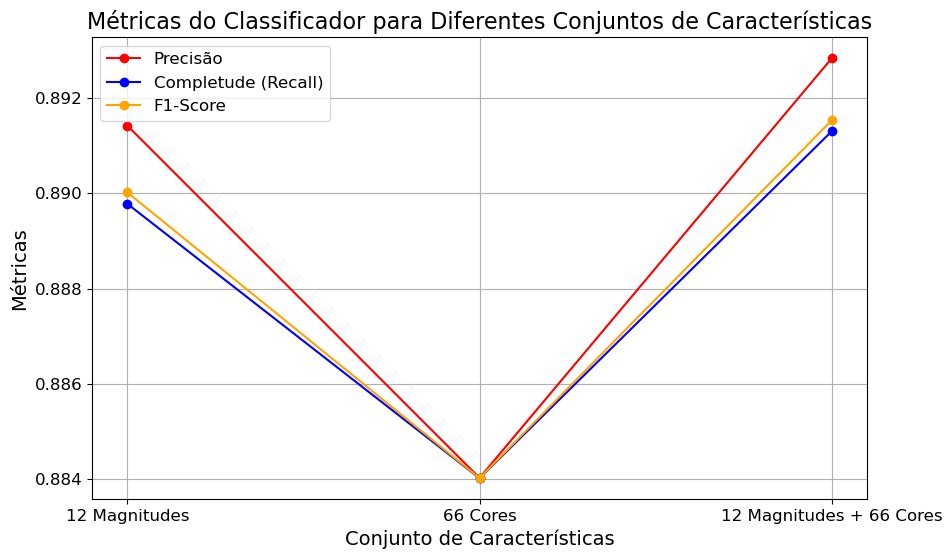
\includegraphics[width=0.8\columnwidth,angle=0]{metricas_comparacao_performace.png}
    \caption[]{Comparação de performance entre os modelos KNN usando apenas as 12 magnitudes, apenas as 66 cores e a combinação de ambas. As métricas apresentadas são: Precisão, Completeza e F1-score.}
    \label{metricas_comparacao_performace}
\end{figure}

O classificador KNN foi treinado com 80\% dos dados (436214 objetos) e testado com os 20\% restantes (109053 objetos), balanceado para garantir que a divisão dos dados entre treinamento e teste preserve a proporção das classes da variável. Isso significa que, se o conjunto de dados original tiver uma distribuição desbalanceada entre as classes (por exemplo, 70\% da classe 0 e 30\% da classe 1), essa mesma proporção será mantida tanto no conjunto de treino quanto no conjunto de teste. No nosso conjunto de treinamento temos um total de 242085 objetos compactos e 194128 objetos extensos, enquanto no conjunto de teste temos 60522 objetos compactos e 48532 objetos extensos.

A seleção dos melhores hiperparâmetros foi realizada por meio de uma busca com o método de \textit{GridSearchCV} da biblioteca \textit{sklearn} em Python, com validação cruzada de 5 folds (cv=5). Esse processo garantiu a otimização dos parâmetros \textit{n\_neighbors}, \textit{metric}, \textit{weights}, \textit{algorithm} e \textit{leaf\_size}, maximizando o desempenho do modelo durante o treinamento.

O modelo final selecionado foi treinado com 27 vizinhos, utilizando a distância de Manhattan como métrica, pesos proporcionais à distância, \textit{algorithm}='auto' e \textit{leaf\_size}=10. Os dados foram normalizados usando a amostra de treino, ajustando sua distribuição para valores entre 0 e 1, de forma a garantir a correta aplicação das métricas de distância. Para isso, utilizamos a função de normalização MinMax do \textit{sklearn} em Python, que transforma os dados para o intervalo [0, 1] com base no conjunto de treinamento. Com esse modelo de normalização salvo, reaplicamos o mesmo modelo nos dados de teste, que também serão usados para as análises posteriores.

\subsection{Análise do classificador}\label{subsec:analise_modelo}
Aplicando o modelo treinado nos dados de teste, podemos realizar e avaliar as previsões feitas pelo classificador. Na Figura \ref{confusion_matrix_knn}, temos a matriz de confusão do modelo, mostrando a quantidade de verdadeiros positivos (TP), verdadeiros negativos (TN), falsos positivos (FP) e falsos negativos (FN) obtidos.

\begin{figure}[!ht]
    \centering
    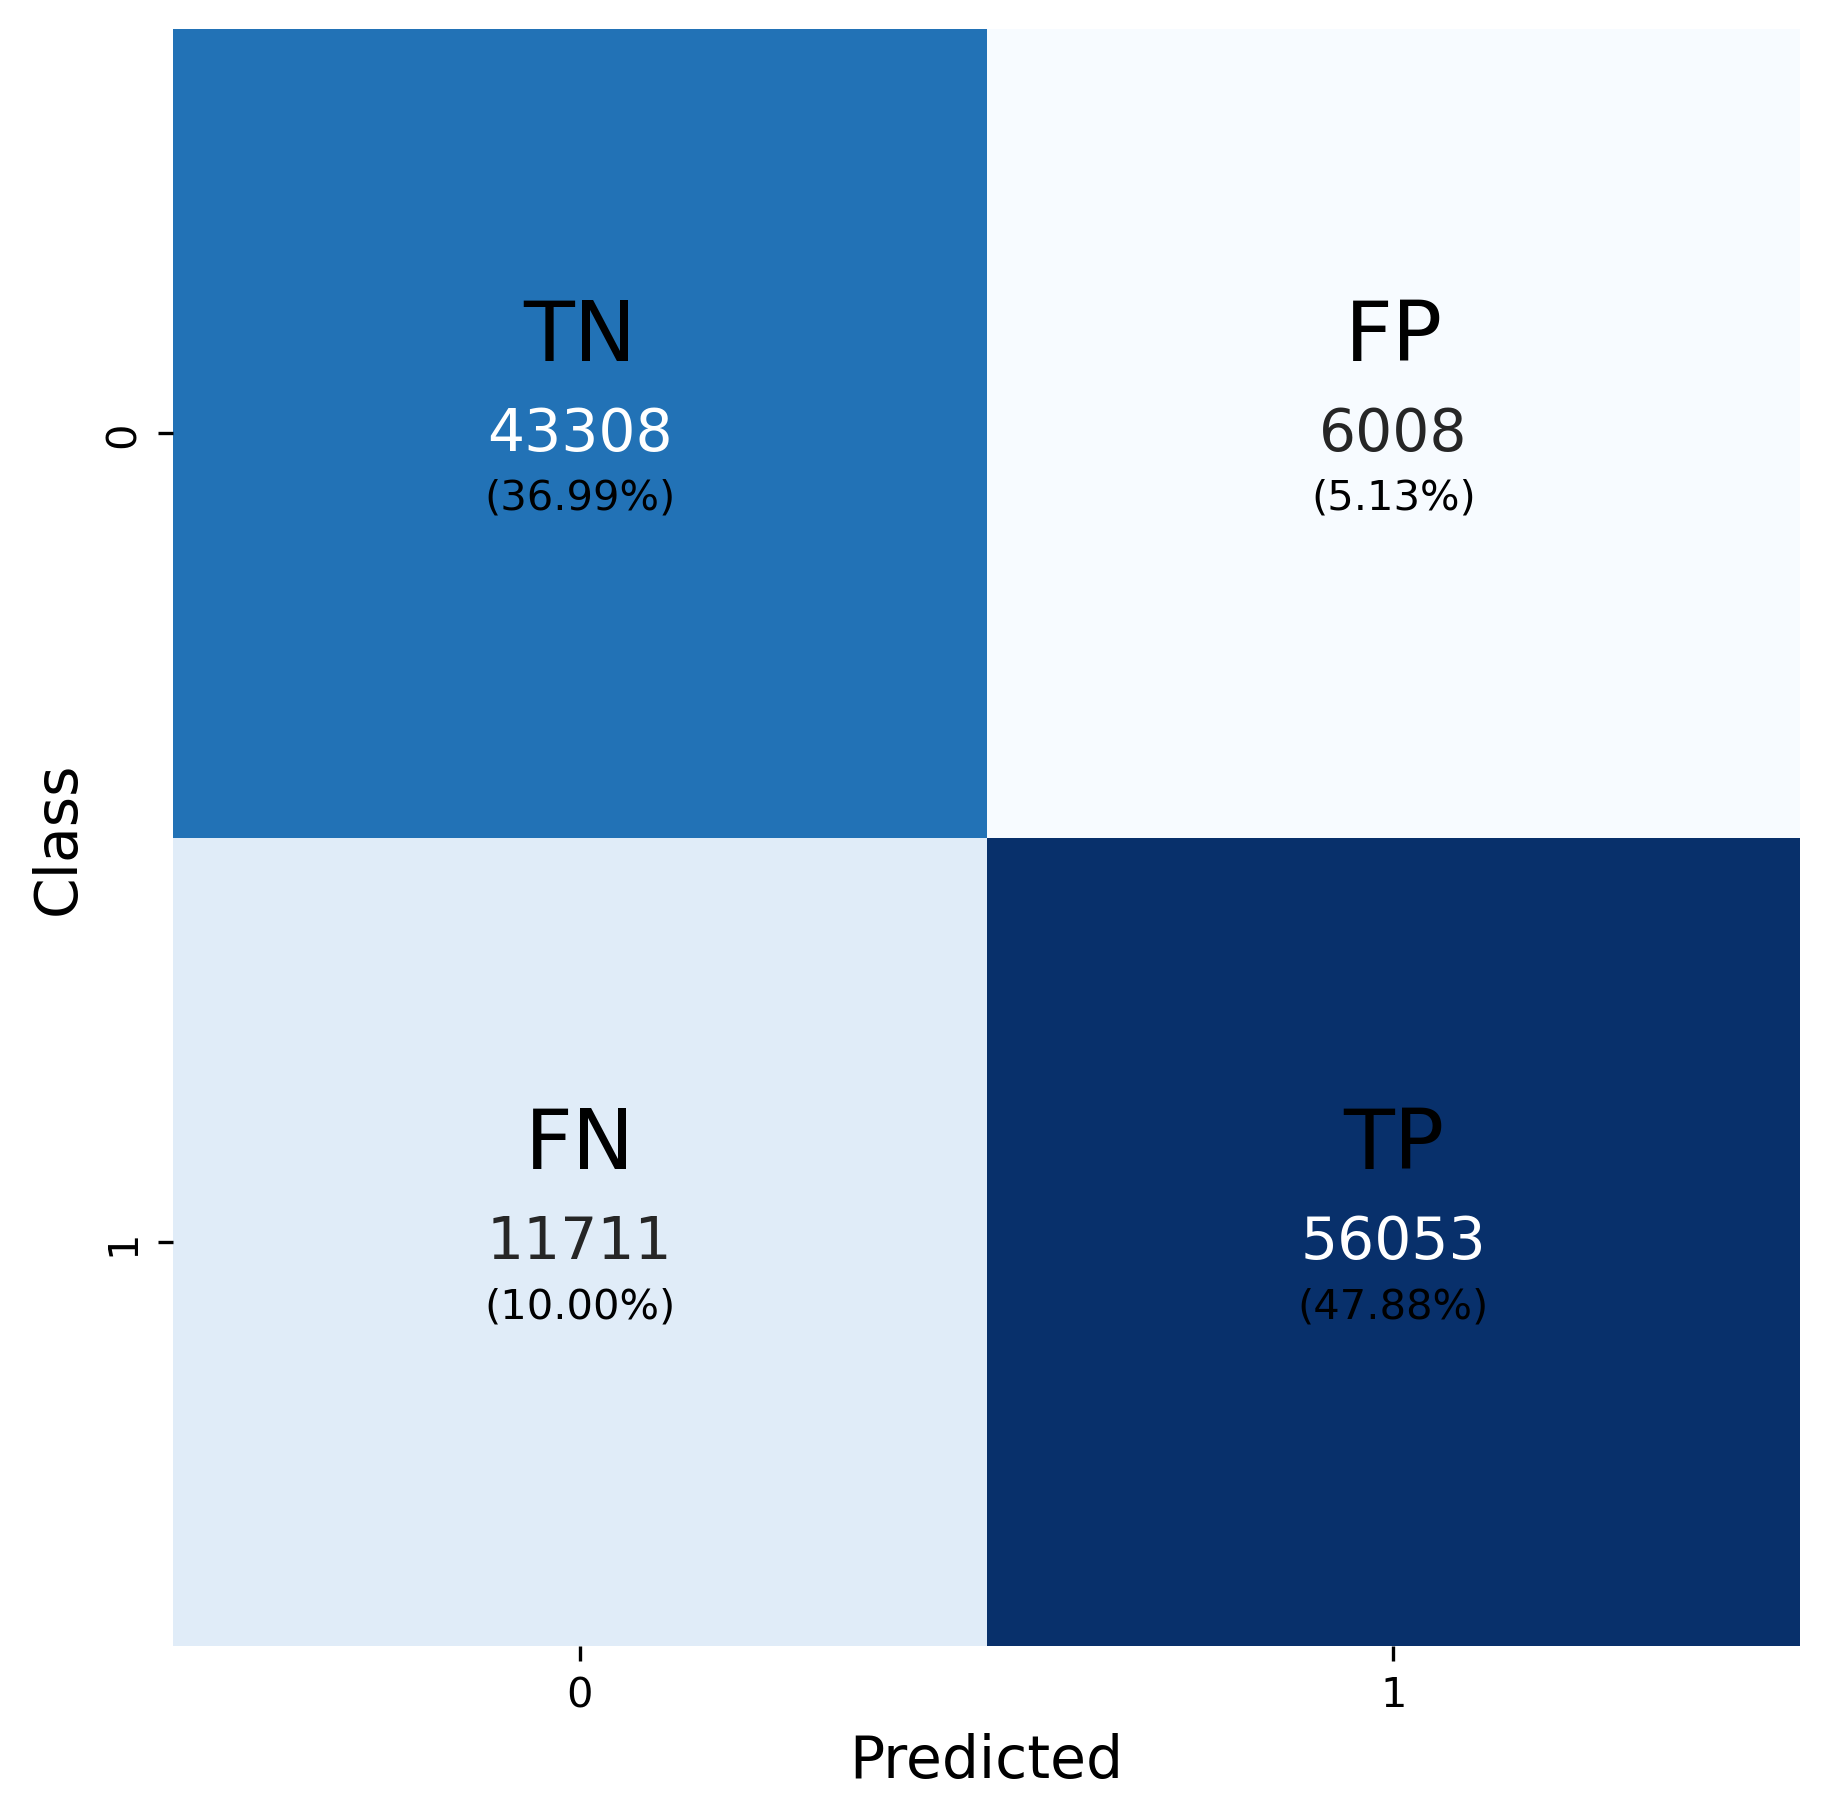
\includegraphics[width=0.5\columnwidth,angle=0]{confusion_matrix_knn.png}
    \caption[]{Matriz de confusão do modelo KNN. A diagonal principal representa os valores corretamente classificados, enquanto os valores fora da diagonal principal representam os erros de classificação das classes 0 e 1.}
    \label{confusion_matrix_knn}
\end{figure}

Muitos dos objetos tiveram classificação correta, como podemos ver na diagonal principal da matriz de confusão. Porém, cabe ressaltar que nem todos os objetos do conjunto de teste eram estrelas ou galáxias, mas sim, majoritariamente, mais de cada um deles nas classes de compactos e extensos, respectivamente. Assim, é esperado que algumas classificações sejam feitas de forma errada, e é nessa proposta que o modelo foi treinado: encontrar aqueles com maior probabilidade de serem extensos, mas que fazem parte do conjunto dos compactos.

Usamos ainda as métricas de acurácia, precisão, completeza e F1-score para avaliar o desempenho do modelo.

A acurácia é definida como a fração das previsões corretas em relação ao total. 

\begin{equation}
    \text{Acurácia} = \frac{TP + TN}{TP + TN + FP + FN}
\end{equation}

A precisão é a fração de verdadeiros positivos em relação ao total de positivos. 

\begin{equation}
    \text{Precisão} = \frac{TP}{TP + FP}
    \label{eq:precisao}
\end{equation}

A completeza é a fração de verdadeiros positivos em relação ao total de positivos previstos.

\begin{equation}
    \text{Completeza} = \frac{TP}{TP + FN}
    \label{eq:completeza}
\end{equation}

O F1-score é a média harmônica entre precisão e completeza.

\begin{equation}
    \text{F1-score} = 2 \times \frac{\text{Precisão} \times \text{Completeza}}{\text{Precisão} + \text{Completeza}}
\end{equation}

Usamos ainda a curva AUC-ROC, amplamente utilizada para modelos de classificação binária. A ROC (Receiver Operating Characteristic) exibe a relação entre a sensibilidade (taxa de verdadeiros positivos) e a taxa de falsos positivos para diferentes valores. A AUC (Área Sob a Curva) resume a performance em um único valor: quanto mais próxima de 1, melhor o modelo diferencia entre as classes. Uma AUC de 0.5 indica classificação aleatória, enquanto 1.0 representa um modelo perfeito.

Essas são as métricas mais populares adotadas em tarefas de classificação binária. Porém, essas medidas estatísticas podem mostrar resultados excessivamente otimistas, especialmente em conjuntos de dados desbalanceados. Uma métrica adicional que usaremos é o coeficiente de correlação de Matthews (MCC), definido por:

\begin{equation}
    \text{MCC} = \frac{TP \times TN - FP \times FN}{\sqrt{(TP + FP)(TP + FN)(TN + FP)(TN + FN)}}
\end{equation}

Ela é uma métrica estatística mais confiável que produz uma pontuação alta apenas se a previsão obtiver bons resultados em todas as quatro categorias da matriz de confusão, proporcionalmente tanto ao tamanho dos elementos positivos quanto ao tamanho dos elementos negativos no conjunto de dados. Os valores do MCC variam de -1 a 1, em que 1 indica uma previsão perfeita, 0 indica uma previsão aleatória e -1 indica uma previsão totalmente incorreta.

A Tabela \ref{metricas_modelo} mostra as métricas obtidas para o modelo KNN treinado.

\begin{table}[!ht]
    \centering
    \caption{Classificação binária - Métricas modelo KNN}
    \begin{tabular}{lccc}
        \toprule
        Classe & Precisão & completeza & F1-Score \\
        \midrule
        0 & 0.90 & 0.63 & 0.74 \\
        1 & 0.87 & 0.97 & 0.92 \\
        \midrule
        \multicolumn{3}{l}{AUC-ROC} & 0.89 \\
        \multicolumn{3}{l}{Coeficiente de Correlação de Matthews (MCC)} & 0.68 \\
        \bottomrule
    \end{tabular}
    \label{metricas_modelo}
\end{table}

Os resultados obtidos têm valores de precisão, completeza e F1-score acima de 0,7 para ambas as classes. A AUC-ROC de 0,89 indica que o modelo é capaz de distinguir entre as duas classes com boa precisão, dadas as limitações dos conjuntos de treinamento. O coeficiente de correlação de Matthews (MCC) de 0,68 é um indicativo de que o modelo é capaz de prever corretamente a maioria dos objetos.

% A principal dificuldade com o classificador está nas regiões onde as classes se sobrepõem no gráfico da Figura \ref{distribution_of_stars_and_galaxies}.
% No entanto, esperamos que o classificador tenha um desempenho melhor nas regiões onde há uma maior concentração de uma única classe no bin de \textit{FWHM}. As classificações e o treinamento do modelo devem refletir essa expectativa.

sobrepõem no gráfico da Figura \ref{distribution_of_stars_and_galaxies}. Foram realizadas as previsões de probabilidade de ser da classe 1 (objetos extensos) para toda a amostra que estaremos analisando na busca (amostra de treino e amostra de teste). A Figura \ref{probabilidade_extensos_fwhm} mostra a distribuição de \textit{FWHM} na banda \textit{r} dos objetos com classificação como estrela ou galáxia do GAIA DR3 com probabilidade maior que 90\%. Sobreposta na imagem, temos matrizes de confusão do classificador para diferentes intervalos de \textit{FWHM}.

\begin{figure}[!ht]
    \centering
    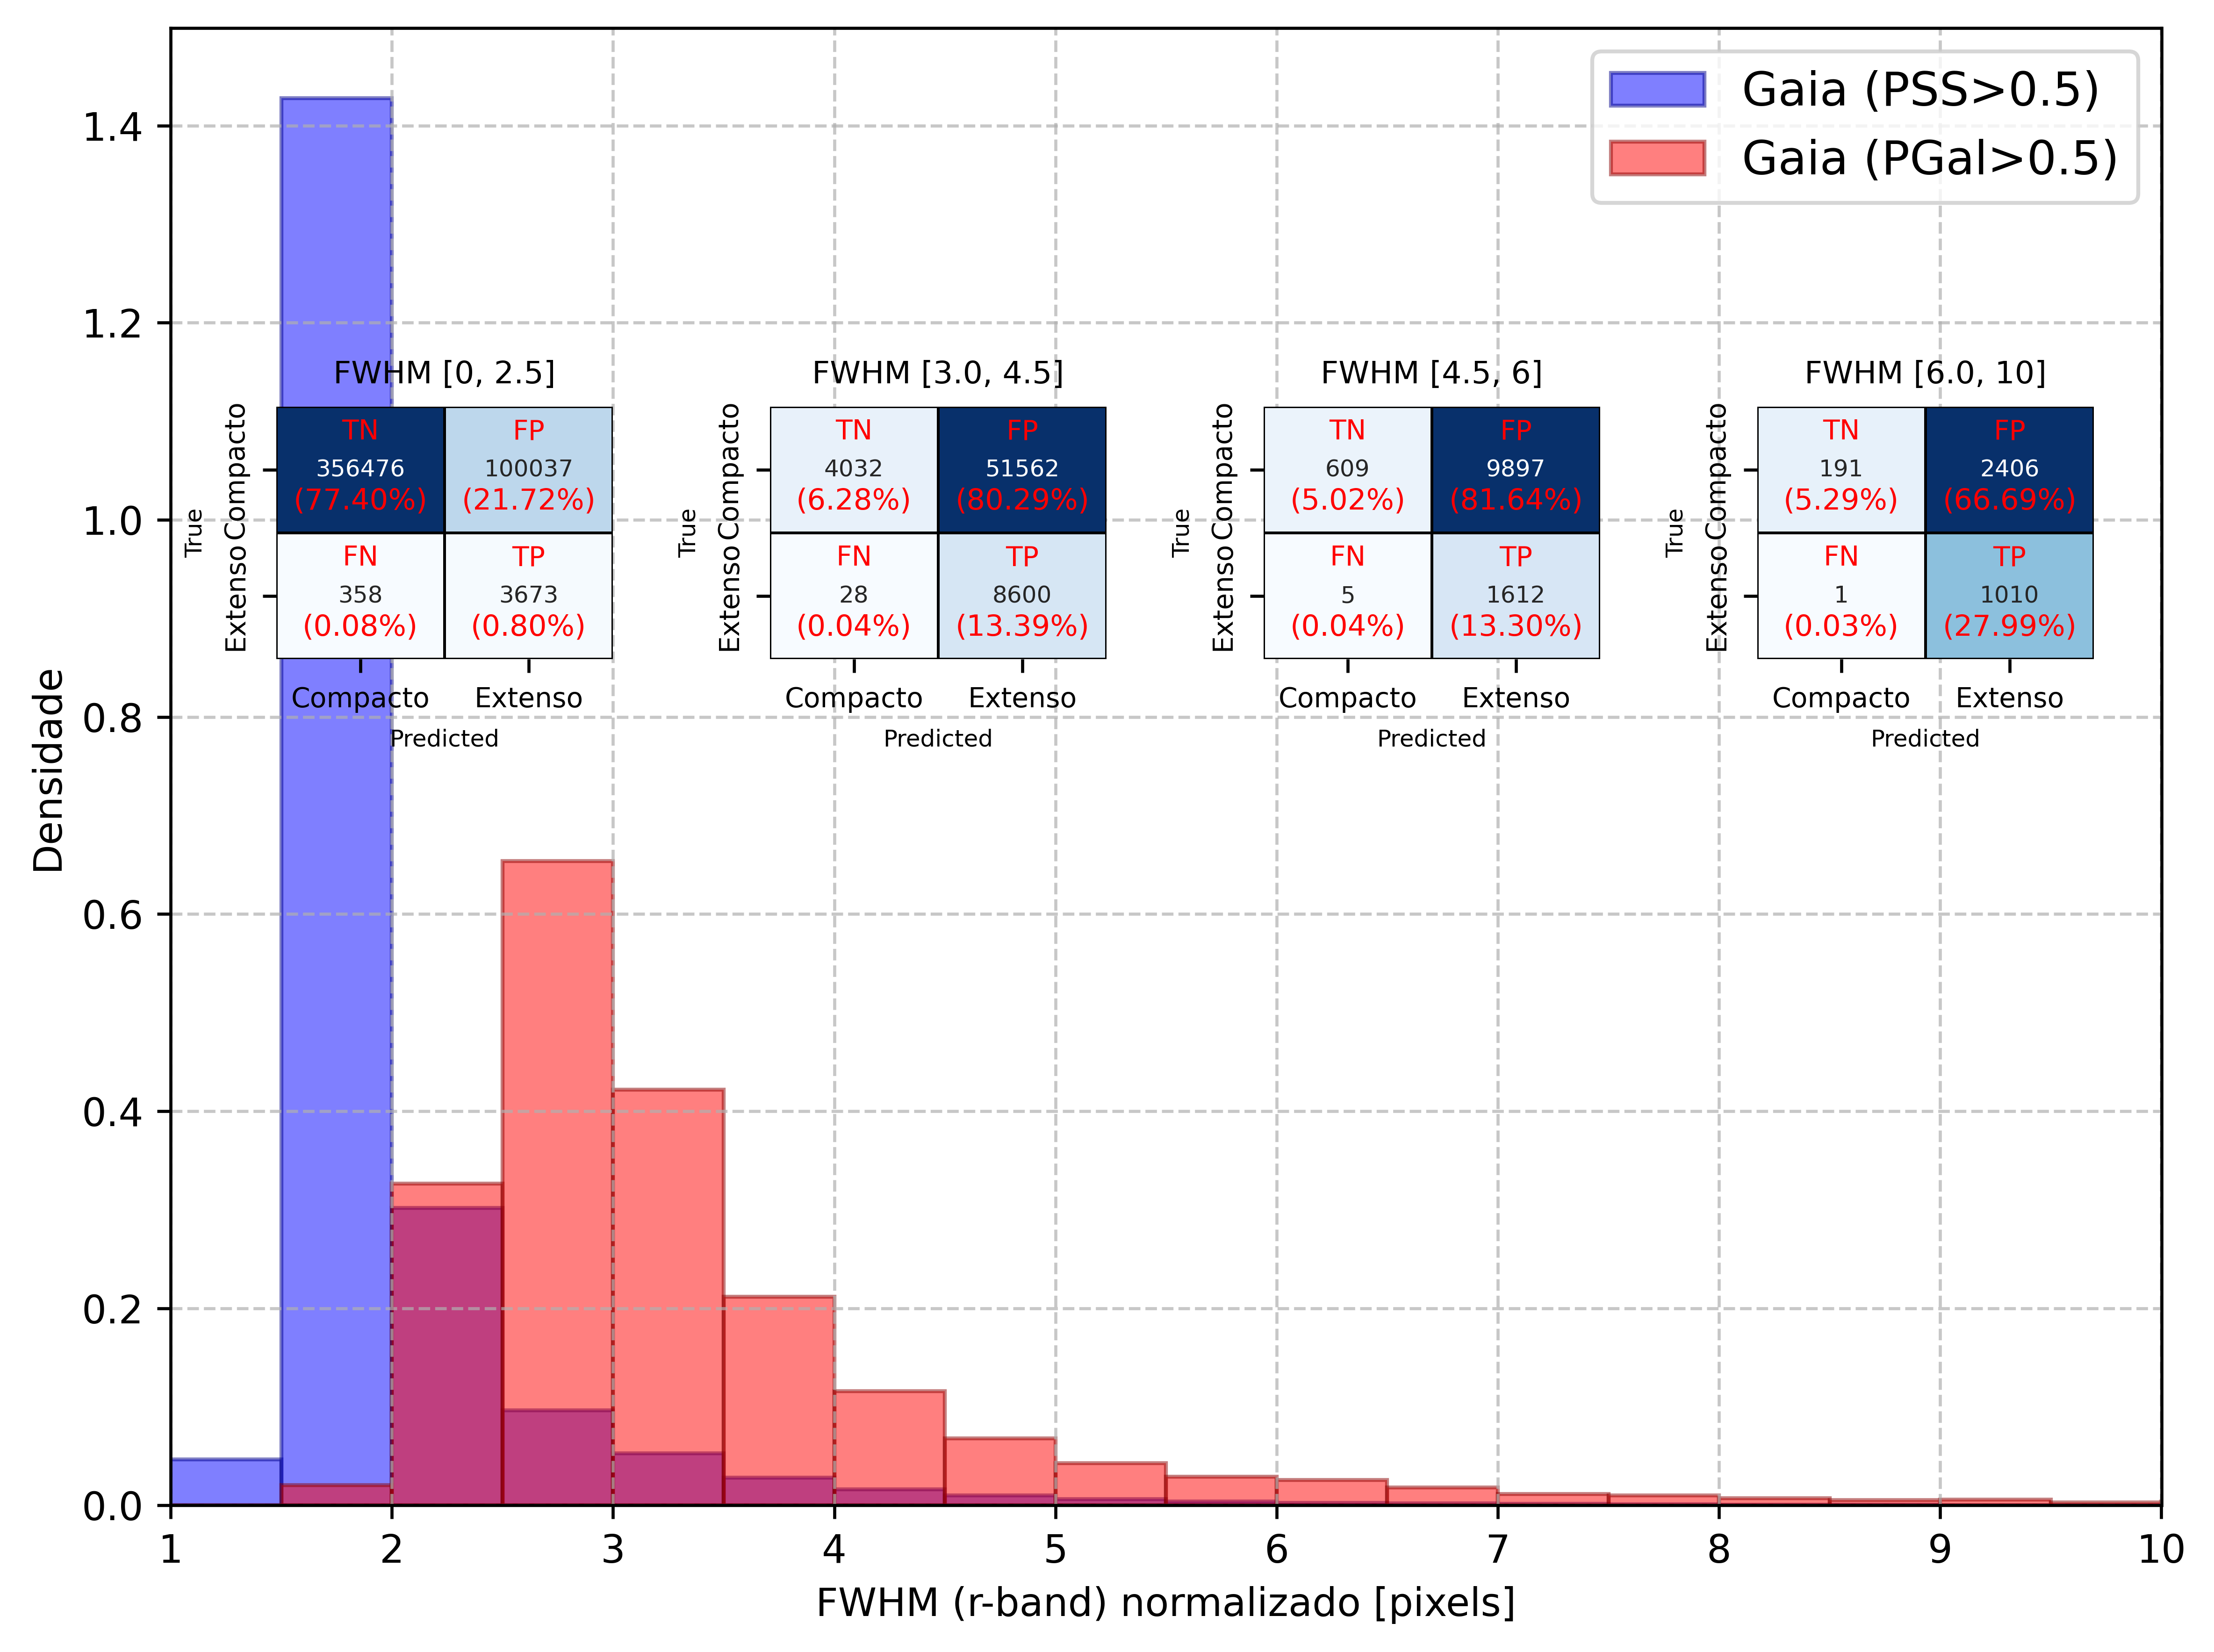
\includegraphics[width=1.\columnwidth,angle=0]{distribution_of_stars_and_galaxies_with_cm.png}
    \caption[]{Distribuição de \textit{FWHM (r-band)} para objetos da amostra com classificação estrela-galáxia do GAIA DR3 com probabilidade maior que 90\%. As matrizes de confusão do classificador KNN para diferentes intervalos de \textit{FWHM} estão sobrepostas. O classificador da a probabilidade de ser da classe 1 (extensos) para cada objeto. }
    \label{probabilidade_extensos_fwhm}
\end{figure}

O comportamento do classificador nas matrizes de confusão mostra que, para as regiões de \textit{FWHM} menores (entre [0, 2.5]), onde há uma maior concentração de estrelas, observa-se uma alta taxa de classificação para objetos do tipo compacto. Já para objetos com \textit{FWHM} maiores, o classificador mostra uma tendência de classificá-los como extensos, o que é esperado, já que esses objetos são menos prováveis de serem estrelas. Para objetos com \textit{FWHM} nas faixas de sobreposição, o desempenho do classificador é misto, refletindo a dificuldade em separar essas classes na região. Porém, é possível observar uma transição gradual entre as classes, consistente com os picos das distribuições de \textit{FWHM}.

Ilustrando ainda o resultado da classificação, apresentamos na Figura \ref{predic_colored} o mesmo gráfico da Figura \ref{amostra_treino} para os objetos da amostra de teste, coloridos de acordo com a probabilidade de serem objetos extensos pelo modelo. A cor azul indica uma probabilidade baixa, enquanto a cor vermelha indica uma probabilidade alta.

\begin{figure}[!ht]
    \centering
    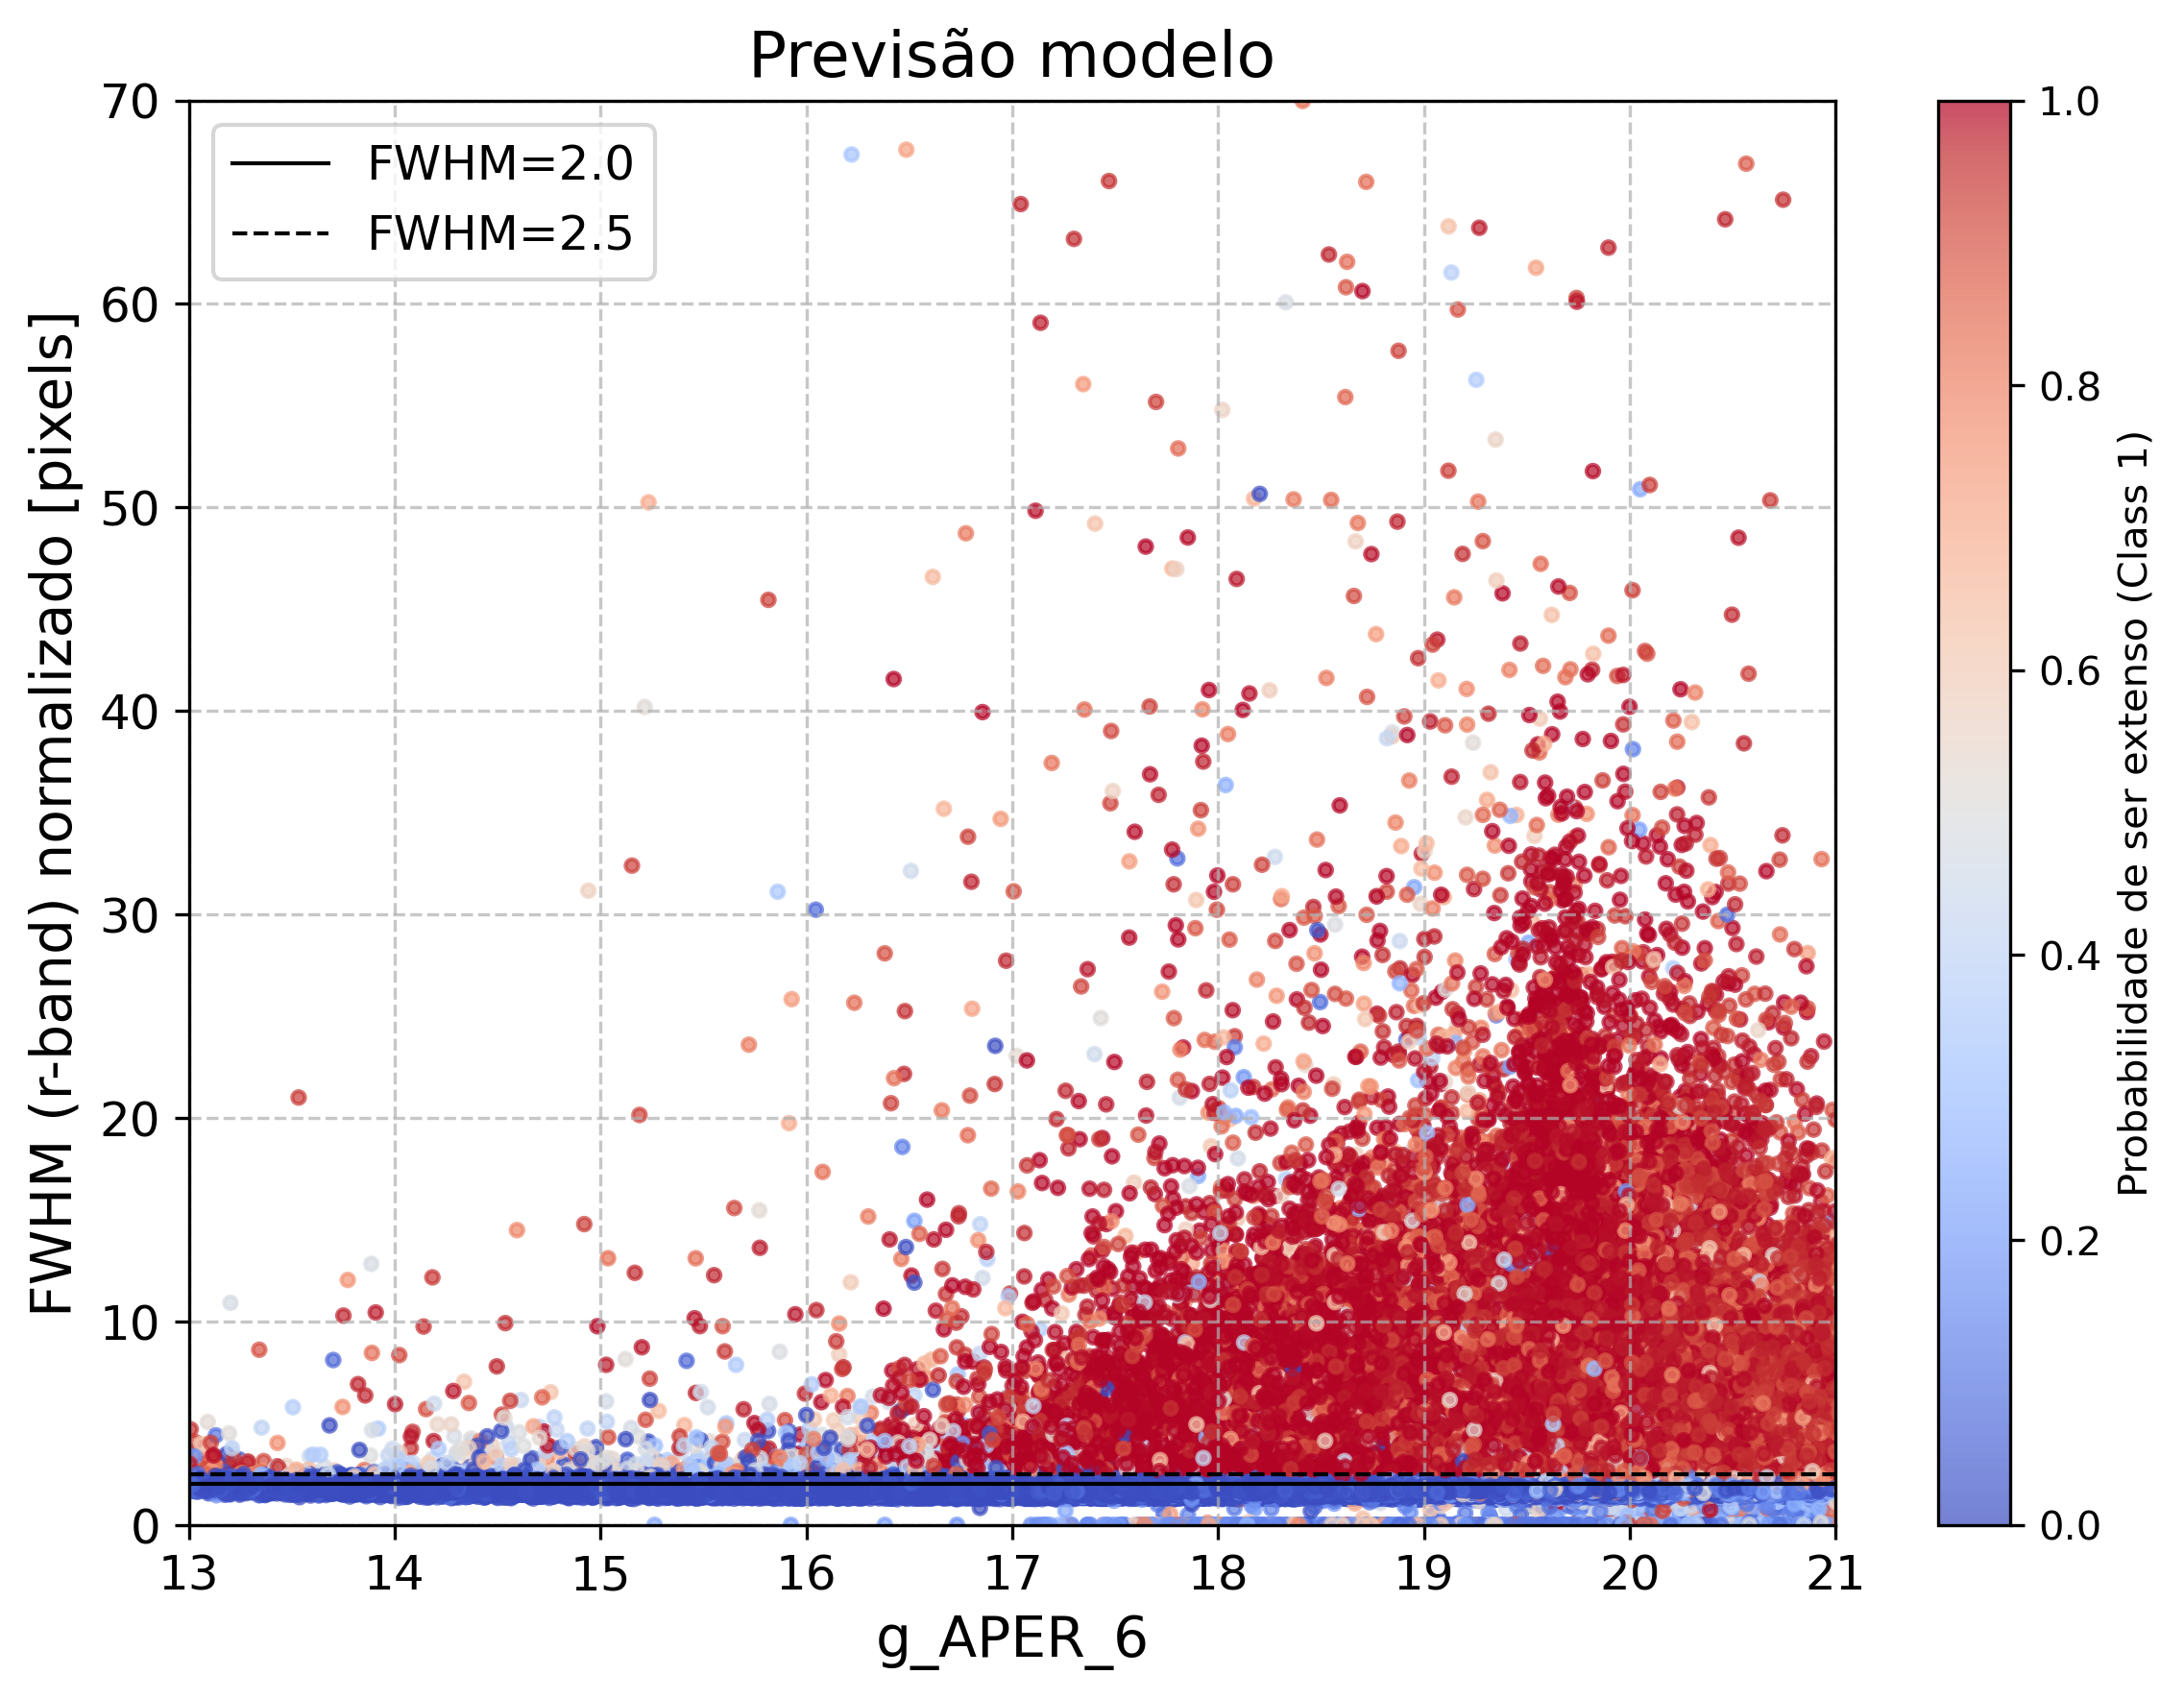
\includegraphics[width=1.\columnwidth,angle=0]{predic_colored.png}
    \caption[]{Distribuição da Largura Total na Metade Máxima (\textit{FWHM} r-band) em função da magnitude \textit{g\_APER\_6} para objetos da amostra de teste, coloridos de acordo com a probabilidade de serem objetos extensos (Classe 1) pelo modelo. Divisão das classes: compactos (\textit{FWHM}$\leq$2 pixels) e extensos (\textit{FWHM}$\geq$2.5 pixels).}
    \label{predic_colored}
\end{figure}

A probabilidade dos objetos serem da classe 1 (objetos extensos) para as UCDs conhecidas na amostra é apresentada na Tabela \ref{ucds_predict}.

\begin{table}[H]
    \centering
    \caption{Classificação do modelo para a classe 1 (objetos extensos) das UCDs na amostra de análise}  
    \begin{tabular}{lc}
        \toprule
        Nome & Predição modelo \\
        \midrule
        UCD3 & 1.00 \\
        UCD1 & 0.77 \\
        F-24 & 1.00 \\
        UCD5 & 0.28 \\
        F-1a & 0.17 \\
        F-9 & 0.95 \\
        F-5 & 0.55 \\
        F-6 & 0.54 \\
        F-7 & 0.85 \\
        F-12 & 0.61 \\
        F-11 & 0.76 \\
        F-34 & 0.91 \\
        F-22 & 0.76 \\
        F-53 & 0.96 \\
        F-51 & 0.96 \\
        F-59 & 0.92 \\
        \bottomrule
    \end{tabular}
    \label{ucds_predict}
\end{table}

Das 16 UCDs presentes, 11 foram classificadas com uma predição acima de 70\%, e 2 com classificação muito pouco provável. Dessa forma, recuperamos a maioria dos objetos de interesse, mostrando a eficácia para buscar novos candidatos na amostra.

\section{Redshifts fotométricos}\label{sec:zphot}

A determinação de redshifts é uma etapa importate para identificar a localização dos objetos no universo. Nesse trabalho, os redshifts fotométricos (\textit{$z_{phot}$}) permite que estimemos a distância dos objetos de forma eficiente e em larga escala, utilizando apenas dados fotométricos. Essa abordagem é especialmente útil quando não há disponibilidade de redshifts espectroscópicos (\textit{$z_{spec}$}), que, embora mais precisos, demandam observações mais demoradas e recursos limitados. A utilização de redshifts fotométricos têm o objetivo de filtrar objetos que não pertencem ao aglomerado de Fornax, reduzindo a contaminação por objetos de fundo.

% Com os objetos filtrados de candidatas, calculamos os redshifts fotométricos (\textit{$z_{phot}$}) dos objetos, selecionando aqueles nos intervalos mais compatíveis com Fornax.

É possível encontrar redshifts fotométricos para parte dos objetos da nossa amostra em outros trabalhos da literatura, assim como em catálogos da própria colaboração S-PLUS \citep{erik_photoz_2024}. Porém, para a busca neste projeto, utilizamos dados com a redução da fotometria do S-PLUS diferentes dos utilizados para os \textit{$z_{phot}$} disponíveis. Assim, mesmo que vindos do mesmo catálogo, uma pequena parte dos objetos na nossa amostra não tem redshifts fotométricos disponíveis. Dos 2900926 objetos iniciais da nossa amostra, 290637 objetos não têm redshifts fotométricos disponíveis em \citep{erik_photoz_2024}, e para eles recalculamos os redshifts fotométricos treinando com nossa amostra.

Abordagens comuns para a estimativa de \textit{$z_{phot}$} incluem o ajuste baseado em modelos espectrais (\textit{template fitting}) e técnicas de aprendizado de máquina. O método de \textit{template fitting} apresenta a vantagem de permitir extrapolações, sendo útil para objetos cujas propriedades não estão bem representadas em amostras conhecidas. Já o aprendizado de máquina tende a ser mais eficiente e preciso quando treinado com um conjunto de dados representativo, embora sua capacidade de generalização seja limitada fora do intervalo coberto pelo treinamento. Além disso, algoritmos de aprendizado de máquina costumam oferecer tempos de inferência mais rápidos, o que os torna especialmente atrativos em contextos com grandes volumes de dados.

Aqui optamos por utilizar o método de aprendizado de máquina para calcular \textit{$z_{phot}$}. Para isso, empregamos modelos de regressão utilizando o algoritmo Random Forest (RF), implementado em Python. No caso da regressão, o RF cria uma floresta de árvores de decisão, onde cada uma delas é treinada com uma amostra aleatória do conjunto inicial dos dados e de seus atributos. A previsão para o valor de \textit{$z_{phot}$} é feita pela média das previsões de cada árvore.

Para a seleção da amostra de treino, utilizamos o mesmo catálogo de Fornax usado anteriormente, com os dados de fotometria do S-PLUS provenientes de \cite{haack2024splusfornaxprojectsfp} (\textit{Run 1}). Ou seja, temos os mesmos dados descritos na seção \ref{sec:Fornax_data}, com as 12 magnitudes corrigidas pela extinção (como descrito na seção \ref{sec:Coeficientes_ext}).

Dessa amostra, selecionamos os objetos com redshifts espectroscópicos disponíveis, provenientes do catálogo \cite{Lima_2024}. Cortamos os objetos em um intervalo de redshifts de 0.002 a 0.5, dessa maneira evitamos boa parte das estrelas (com redshifts menores) e galáxias muito distantes de Fornax. Cortamos também em um intervalo de magnitude de \textit{r\_APER\_6}$\geq$15 e \textit{r\_APER\_6}$\leq$21, evitando objetos muito brilhantes e saturados, e objetos com baixa qualidade de medição, respectivamente.

Removemos também os objetos com medições faltantes em alguma das 12 magnitudes das aberturas \textit{APER\_6}, resultando em uma amostra final com 12.296 objetos.

Para o treinamento, os melhores resultados a princípio se deram com a utilização das combinações das 66 cores das 12 magnitudes de abertura \textit{APER\_6}. Assim, treinamos o modelo fornecendo o redshift espectroscópico (\textit{$z_{spec}$}) como variável alvo e as 66 cores como variáveis preditoras.

% A seleção dos melhores hiperparâmetros foi realizada com validação cruzada de 5 folds, otimizando os parâmetros \textit{n\_neighbors}, \textit{metric}, \textit{weights}, \textit{algorithm} e \textit{leaf\_size}.

O conjunto de dados foi normalizado com usando a amostra de treino, ajustando sua distribuição para valores entre 0 e 1 pela função MinMax do python. Além disso, dividimos a amostra em 80\% para treino e 20\% para teste.

A Figura \ref{zphot_zspec} mostra a comparação entre os redshifts espectroscópicos (\textit{$z_{spec}$}) e fotométricos (\textit{$z_{phot}$}) para a amostra de treino. A linha tracejada representa a relação 1:1 entre os redshifts, enquanto a linha contínua representa a relação ajustada pelo modelo de regressão.

\begin{figure}[!ht]
    \centering
    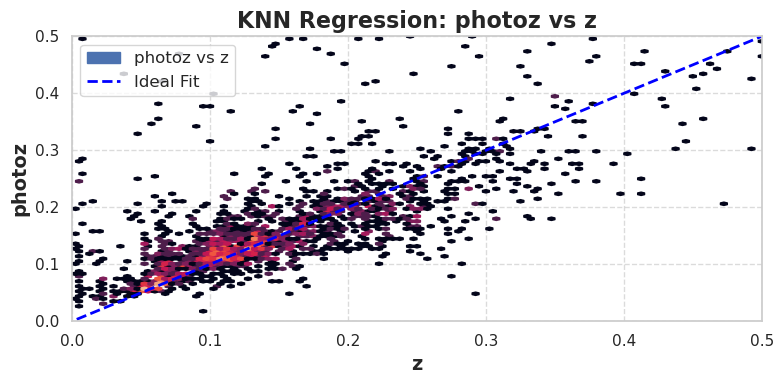
\includegraphics[width=1.\columnwidth,angle=0]{zphot_zspec.png}
    \caption[]{Resultados da regressão com o algoritmo Random Forest (RF) para estimar os redshifts fotométricos (\textit{$z_{phot}$}) em relação aos redshifts espectroscópicos (\textit{$z_{spec}$}). Na parte superior, o gráfico de dispersão compara \textit{$z_{phot}$} vs \textit{$z_{spec}$}. A linha azul tracejada representa o ajuste ideal (\textit{$z_{phot}$} = \textit{$z_{spec}$}). A densidade de pontos é representada por um gradiente de cores, com áreas mais densas indicadas em tons mais claros. Na parte inferior, o gráfico de resíduos exibe a diferença entre \textit{$z_{phot}$} e \textit{$z_{spec}$}. A linha preta tracejada representa a linha zero.}
    \label{zphot_zspec}
\end{figure}

Percebemos pela Figura \ref{zphot_zspec} que o modelo de regressão foi capaz de estimar os redshifts fotométricos com certa precisão. As métricas que adotamos para avaliar o desempenho do modelo foram o erro quadrático médio (EQM), o $R^2$ o $\sigma_{nmad}$ e a fração de outliers (Fout). O EQM é uma medida da média dos erros quadráticos entre os valores previstos e os valores reais. O $R^2$ é uma medida de quão bem os dados se ajustam ao modelo, variando de 0 a 1, onde 1 indica um ajuste perfeito. O $\sigma_{nmad}$ é uma medida robusta de dispersão que quantifica a variação dos resíduos em relação à mediana. A fração de outliers (Fout) é a proporção de previsões que estão além de um certo limite em relação aos valores reais.

Os resultados obtidos para essas métricas foram: EQM = 0,05, $R^2$ = 0,6, $\sigma_{nmad}$ = 0,03 e Fout = 0,08. Embora os valores indiquem uma precisão moderada, o modelo apresenta algumas estimativas com erros maiores, especialmente para redshifts mais elevados. É importante destacar que o objetivo principal deste modelo não é fornecer redshifts altamente precisos para todos os objetos, mas sim identificar aqueles com redshifts compatíveis com o aglomerado de Fornax. Dessa forma, mesmo com a presença de erros, o modelo é útil para filtrar objetos com maior probabilidade de pertencerem ao fundo, proporcionando um ganho significativo na seleção de candidatos.

Aplicando o modelo para as UCDs conhecidas em Fornax, obtivemos os resultados apresentados na Tabela \ref{ucds_zphot}, juntamente com os redshifts fotométricos fornecidos por \cite{erik_photoz_2024} (\textit{zml}). Para os objetos que possuem redshifts fotométricos disponíveis em \cite{erik_photoz_2024}, observamos que esses valores são mais precisos e compatíveis com os esperados para Fornax, em comparação com os redshifts fotométricos estimados pelo nosso modelo.

Essa diferença de desempenho é compreensível, dado que o modelo de \cite{erik_photoz_2024} utiliza uma abordagem mais robusta, baseada em uma amostra maior de objetos com redshifts espectroscópicos conhecidos, o que proporciona maior confiabilidade nos resultados. Por outro lado, nosso modelo, embora tenha apresentado resultados razoáveis, é limitado pela menor quantidade de dados disponíveis para o treinamento.

Portanto, concluímos que, sempre que possível, os cortes baseados em redshifts fotométricos devem ser realizados utilizando os valores de \cite{erik_photoz_2024}. Para os casos em que esses dados não estão disponíveis, utilizaremos os redshifts fotométricos estimados pelo nosso modelo como uma alternativa, cientes de suas limitações.

\begin{table}[!ht]
    \centering
    \caption{Aplicação do modelo de regressão para estimativas de redshifts fotométricos para UCDs conhecidas na amostra de análise de Fornax (\textit{$z_{phot}$}), junto com as previsões de \citep{erik_photoz_2024} (\textit{zml}), para aqueles objetos que tinham dados presentes e o redshift espectroscópico (\textit{$z_{spec}$}) disponível.}
    \begin{tabular}{lccc}
        \toprule
        Nome & \textit{$z_{phot}$} & \textit{zml} & \textit{$z_{spec}$}\\
        \midrule
        UCD3 & 0.07 & 0.03 & 0.0053\\
        UCD1 & 0.09 & 0.08 & 0.0052\\
        F-24 & 0.08 & 0.04 & 0.0062\\
        UCD5 & 0.03 & 0.04 & 0.0045\\
        F-1a & 0.21 & -- & --\\
        F-9 & 0.09 & 0.07 & 0.0058\\
        F-5 & 0.06 & -- & 0.0057\\
        F-6 & 0.10 & -- & 0.0037\\
        F-7 & 0.19 & 0.16 & --\\
        F-12 & 0.07 & -- & 0.0055\\
        F-11 & 0.10 & -- & 0.0059\\
        F-34 & 0.07 & -- & 0.0054\\ 
        F-22 & 0.09 & 0.06 & 0.0034\\
        F-53 & 0.31 & -- & 0.0020\\
        F-51 & 0.10 & -- & 0.0041\\
        F-59 & 0.06 & -- & 0.0060\\
        \midrule
    \end{tabular}
    \label{ucds_zphot}
\end{table}

Nosso objetivo não é estimar redshifts precisos para todos os objetos, mas sim aplicar um corte que nos ajude a remover objetos com maiores chances de serem do fundo. Sabendo que o redshift de Fornax é de aproximadamente $0.005$\footnote{https://simbad.u-strasbg.fr/simbad/sim-id?Ident=Fornax+Cluster}, e observando os redshifts fotométricos estimados para as UCDs conhecidas, podemos adotar um corte conservador para os redshifts fotométricos, com uma margem otimista para o erro.

\section{Seleção das candidatas}\label{cap:selecao_candidatas}
Para a seleção das candidatas, queremos primeiramente criar uma subamostra dos dados de Fornax, contendo os objetos compactos de nosso interesse. A partir dessa amostra, iremos selecionar pelas probabilidades de serem extensos (classe 1).

A partir de \cite{Su_2021}, removemos os objetos confirmados espectroscopicamente como sendo do background. Usando o catálogo de redshifts espectroscópicos de \cite{Lima_2024}, removemos os objetos que possuem redshifts maiores que 0.0055, considerando que esses objetos estão mais distantes de Fornax e, portanto, não pertencem ao aglomerado.

Pela Figura \ref{distribuicao_fwhm_image_r_r_aper6_ucds_fornax}, das UCDs conhecidas em Fornax, cortamos pela magnitude \textit{r\_APER\_6}$\geq$17, correspondendo a 0.5 magnitudes de diferença da UCD mais brilhante no intervalo. Cortamos também \textit{g\_APER\_6}$\leq$21, para evitar a contaminação de aglomerados globulares.

Das 16 UCDs conhecidas em Fornax, temos o maior \textit{FWHM (r-band)} para a \textit{F-34} com 3.68 pixels, sendo ela a única exceção, com todas as outras 15 com \textit{FWHM (r-band)} menor que 3.2 pixels. Para a seleção e otimização da maior quantidade de objetos compactos, cortamos na mesma definição que usamos para separação de objetos extensos e compactos, vindas da seção \ref{subsec:amostra_treino}, com \textit{FWHM (r-band)}$\leq$2.5 pixels.

Uma das contaminações que queremos remover em nossa amostra é a de estrelas. Elas representam uma fração significativa, tornando essencial sua remoção, reduzindo o número de objetos não interessantes na amostra final.

Poderíamos utilizar uma classificação externa, como o classificador estelar do Gaia DR3. No entanto, conforme mostrado na seção \ref{sec:ucds_fornax}, algumas UCDs conhecidas são classificadas incorretamente, especialmente as mais fracas. Por isso, optamos por definir um corte em parâmetros da amostra que nos ajude a remover parte das estrelas mais evidentes.

{\sloppy
Usando os parâmetros \text{FLUX\_RADIUS\_90}, \text{FLUX\_RADIUS\_70}, \text{FLUX\_RADIUS\_50} e \text{FLUX\_RADIUS\_20}, que correspondem à medida em pixels do raio que contém 90\%, 70\%, 50\% e 20\% do fluxo total da fonte, respectivamente, esperamos que as UCDs tenham uma distribuição mais pontual. Dessa forma, em diferentes aberturas, por exemplo, entre 90\% e 70\%, devemos esperar que existam certas diferenças nas distribuições de luz das UCDs, estrelas e algumas galáxias mais extensas. Com essa ideia, criamos alguns gráficos com as melhores combinações de parâmetros que ajudam a remover a contaminação na amostra. Mostramos nas Figuras \ref{flux_radius_1}, \ref{flux_radius_2} e \ref{flux_radius_3} os três gráficos com a combinação de parâmetros. As classificações que apresentamos neles são as do GAIA DR3, com probabilidade maior que 90\% de serem estrelas ou galáxias. Os pontos em azul representam as estrelas, em vermelho as galáxias e em preto as UCDs conhecidas.}

Em cada uma das três figuras, foram delimitadas visualmente duas retas, separando as fronteiras entre galáxias e estrelas. Assim, foram definidos seis cortes adicionais para remover a contaminação de candidatas indesejadas. A Tabela \ref{cortes_flux_radius} apresenta os cortes aplicados às retas dos gráficos \ref{flux_radius_1}, \ref{flux_radius_2} e \ref{flux_radius_3}. Nas colunas, $FR$ é a abreviação de FLUX\_RADIUS, na banda $r$ e abertura $APER\_6$. Eles representam o raio em que a porcentagem do fluxo total da fonte se encontra. Os parâmetros com porcentagem entre parênteses representam a diferença entre os dois valores. Entre os parâmetros, temos os valores de $a$ e $b$ para a equação da reta $y = ax + b$. 

Observamos nesses gráficos que a maioria das estrelas está concentrada em regiões mais externas. Embora tenhamos utilizado a própria classificação estelar do GAIA DR3, que, como discutido anteriormente, não é perfeita para nossos objetos mais fracos, esses cortes contribuirão para remover a maior parte das estrelas sem comprometer a seleção de UCDs.

Além disso, os gráficos mostram que as UCDs conhecidas ocupam as mesmas regiões que as galáxias, juntamente com algumas estrelas que seguem uma distribuição semelhante. Dessa forma, destacamos que esses cortes, mesmo sendo relativamente abrangentes, permitem reduzir a contaminação estelar sem impactar negativamente nosso objetivo.

\begin{table}[!ht]
    \centering
    \caption{Combinações das variáveis para os cortes das retas dos gráficos \ref{flux_radius_1}, \ref{flux_radius_2} e \ref{flux_radius_3}. Nas colunas, FR é a abreviação de FLUX\_RADIUS, na banda $r$ e abertura $APER\_6$. Eles representam o raio em que a porcentagem do fluxo total da fonte se encontra. Os parâmetros com porcentagem entre parênteses representam a diferença entre os dois valores. Entre os parâmetros, temos os valores de $a$ e $b$ para a equação da reta $y = ax + b$. }
        \begin{tabular}{l l r r}
        \hline
        \multicolumn{4}{c}{$y = ax + b$}\\
        \hline
        y & x & a & b\\
        \hline
        FR (90\%-20\%) & r & -4.5 & 97 \\
        FR (90\%-20\%) & r & -0.8 & 17 \\
        FR (90\%-70\%) & FR 90\% & 0.7 & -0.8 \\
        FR (90\%-70\%) & FR 90\% & 0.3 & -0.45 \\
        FR (70\%-20\%) & FR (90\%-70\%) & 1.6 & 1 \\
        FR (70\%-20\%) & FR (90\%-70\%) & 0.4 & 0.05 \\
        \hline
    \end{tabular}
    \label{cortes_flux_radius}
\end{table}

\begin{figure}[!ht]
    \begin{center}
    % \setcaptionmargin{1cm}
    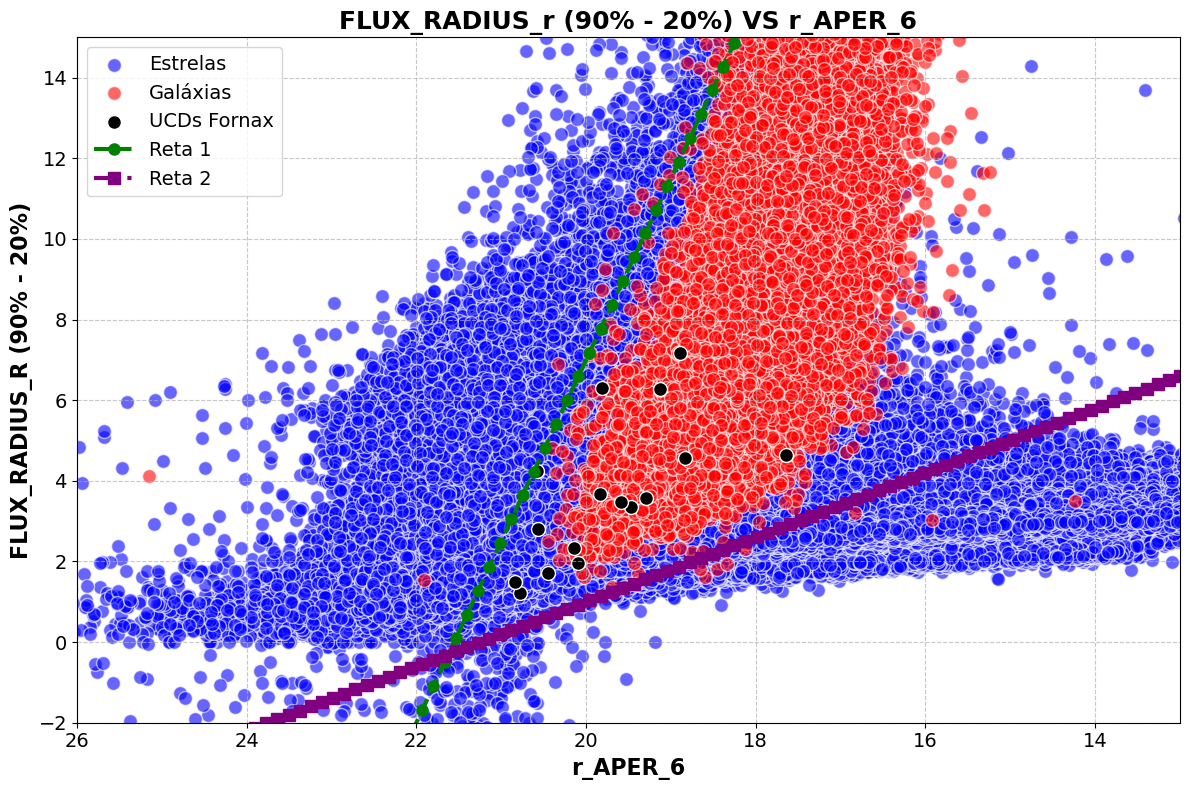
\includegraphics[width=0.8\columnwidth,angle=0]{f_90_20_R_APER_6.png}
    \caption{Gráfico de \text{FLUX\_RADIUS\_90} - \text{FLUX\_RADIUS\_20} em função de \text{r\_APER\_6} para objetos da amostra com classificação estrela-galáxia do GAIA DR3 com probabilidade maior que 90\%. Pontos em azul representam as estrelas, em vermelho as galáxias e em preto as UCDs. As retas em verde e roxo representam os cortes para remover a contaminação de estrelas.}
    \label{flux_radius_1}
    \end{center}
\end{figure}

\begin{figure}[!ht]
    \begin{center}
    % \setcaptionmargin{1cm}
    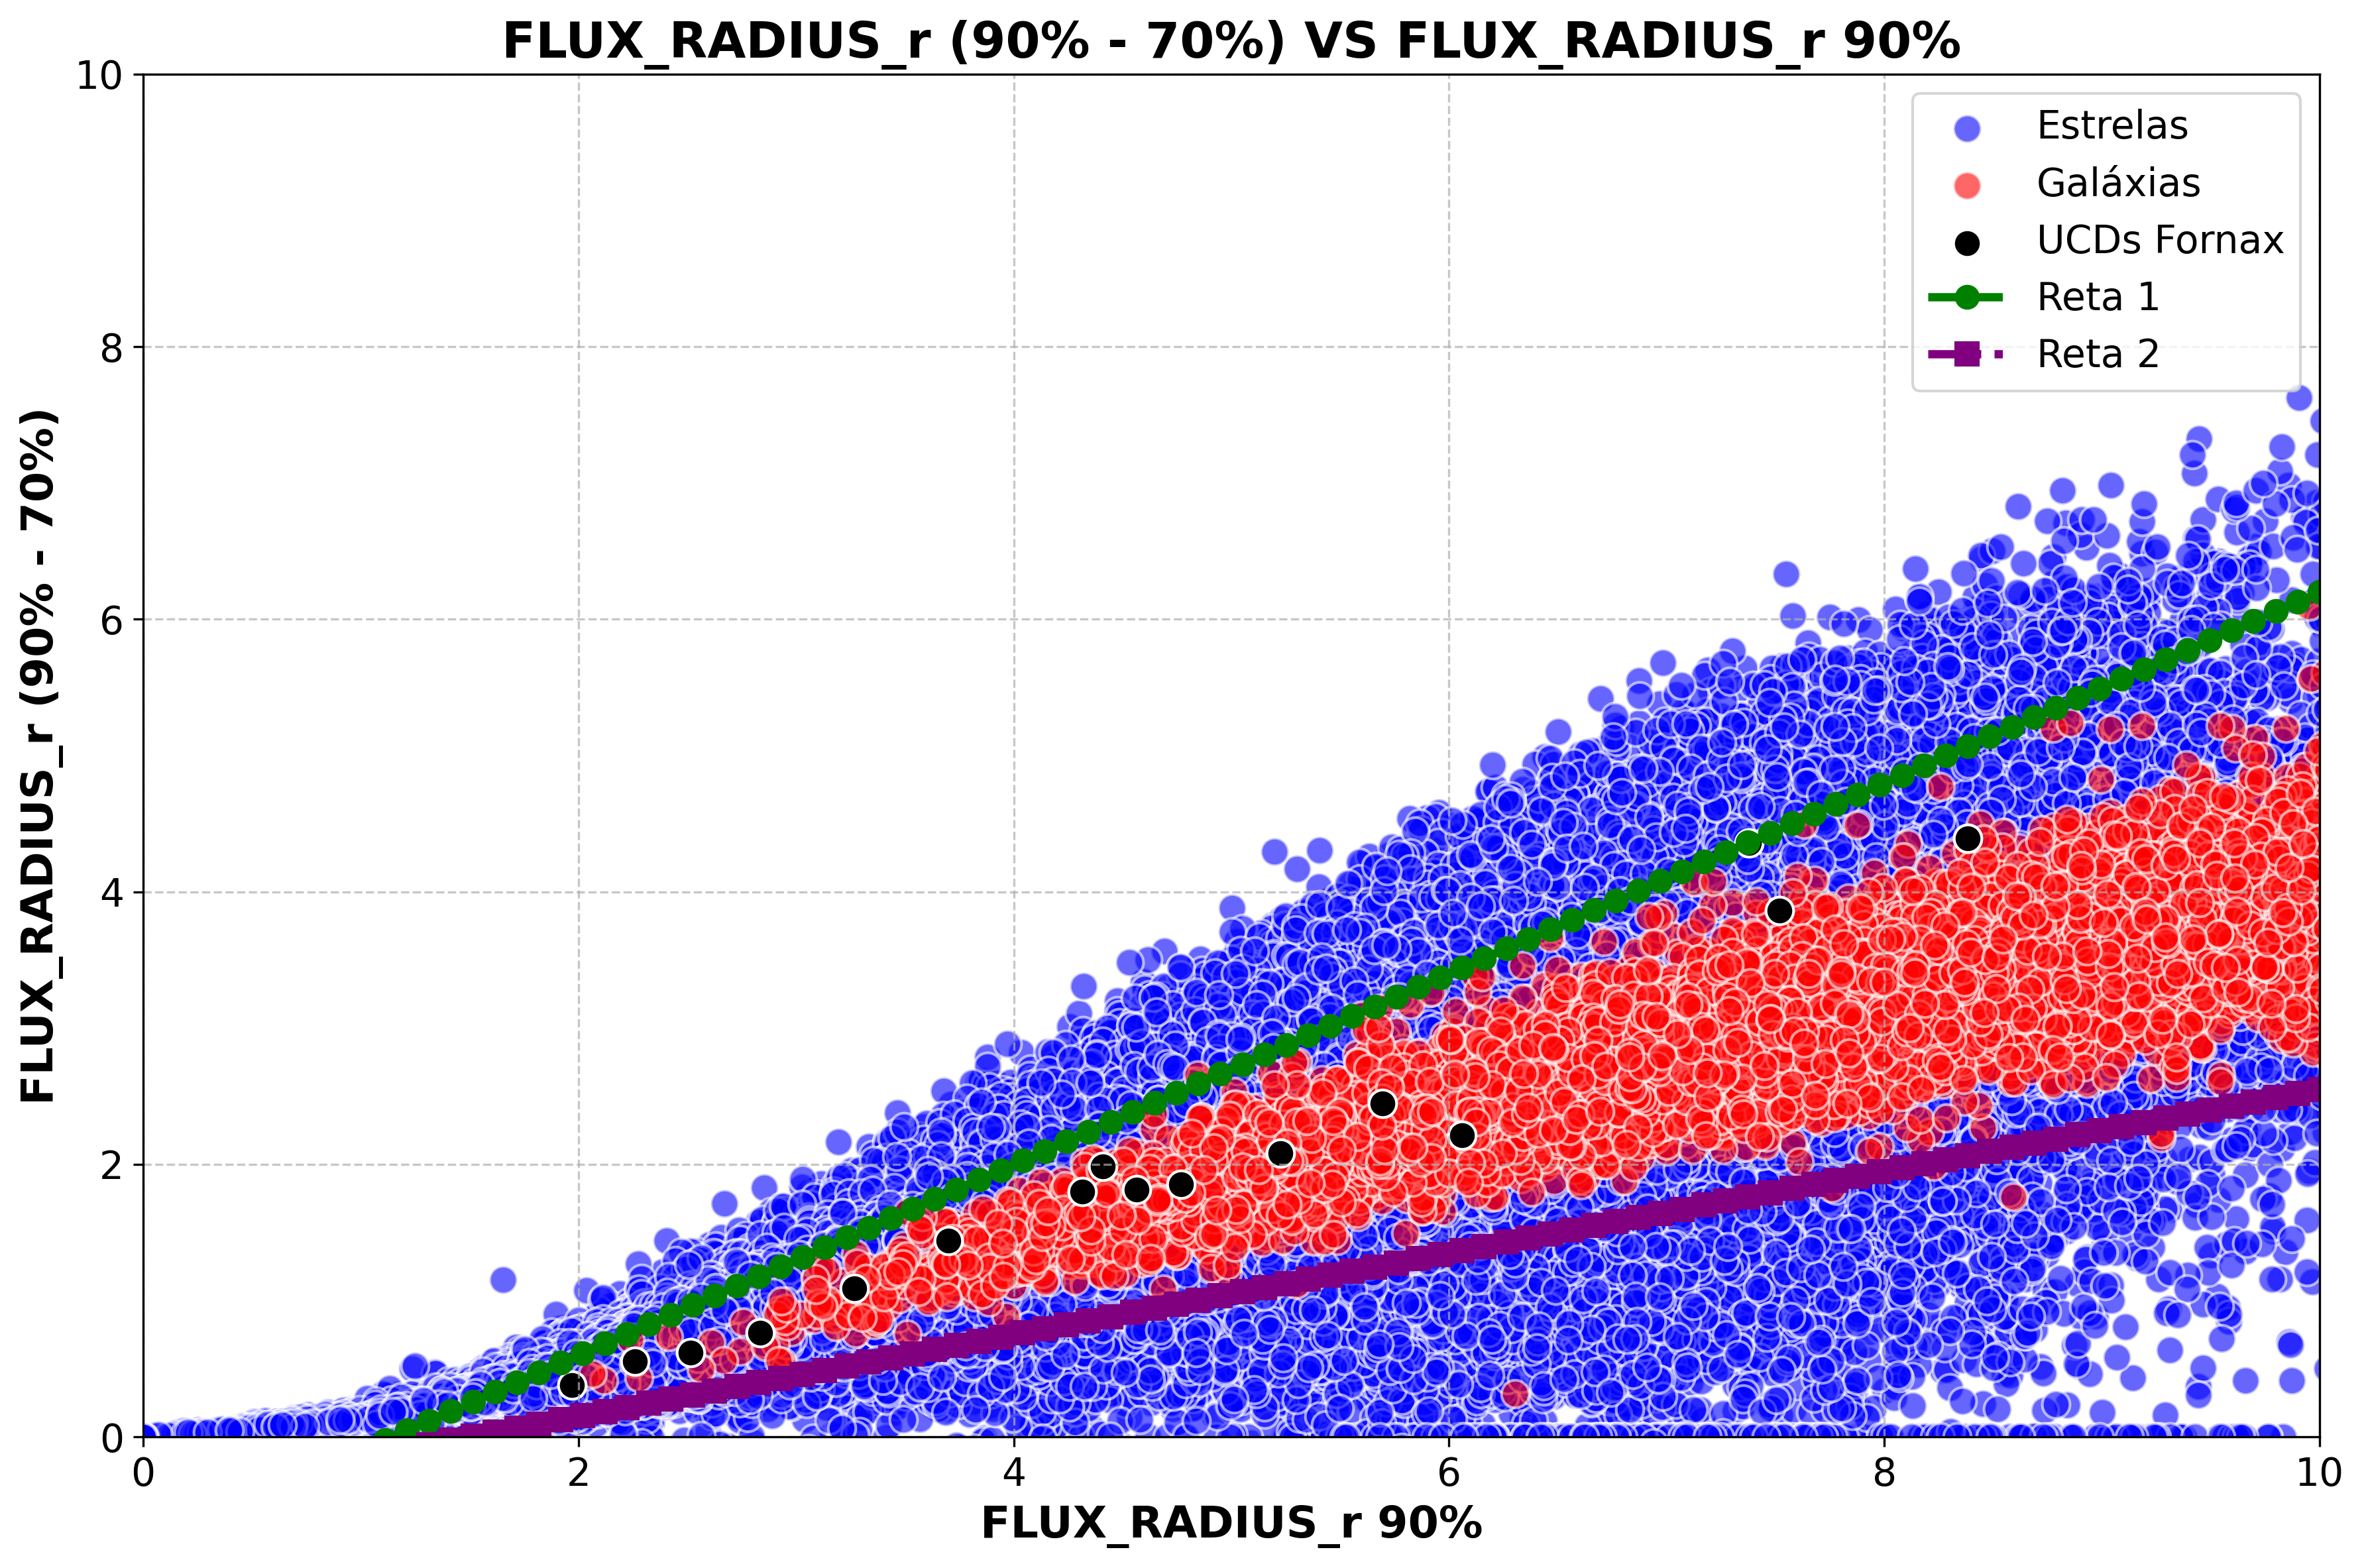
\includegraphics[width=0.8\columnwidth,angle=0]{f_90_70_FLUX_RADIUS_90_R.png}
    \caption[]{Gráfico de \text{FLUX\_RADIUS\_90} - \text{FLUX\_RADIUS\_70} em função de \text{FLUX\_RADIUS\_90} para objetos da amostra com classificação estrela-galáxia do GAIA DR3 com probabilidade maior que 90\%. Pontos em azul representam as estrelas, em vermelho as galáxias e em preto as UCDs. As retas em verde e roxo representam os cortes para remover a contaminação de estrelas.}
    \label{flux_radius_2}
    \end{center}
\end{figure}

\begin{figure}[!ht]
    \begin{center}
    % \setcaptionmargin{1cm}
    \includegraphics[width=0.8\columnwidth,angle=0]{f_70_20_f_90_70.png}
    \caption[]{Gráfico de \text{FLUX\_RADIUS\_70} - \text{FLUX\_RADIUS\_20} em função de \text{FLUX\_RADIUS\_90} - \text{FLUX\_RADIUS\_70} para objetos da amostra com classificação estrela-galáxia do GAIA DR3 com probabilidade maior que 90\%. Pontos em azul representam as estrelas, em vermelho as galáxias e em preto as UCDs. As retas em verde e roxo representam os cortes para remover a contaminação de estrelas.}
    \label{flux_radius_3}
    \end{center}
\end{figure}

Depois desses cortes para seleção de objetos compactos, com base nas classificações do modelo, filtramos aqueles com probabilidade maior que 90\% de serem extensos. A partir dessa amostra, selecionamos as candidatas a UCDs, que são objetos compactos com alta probabilidade de serem extensos.

Fazendo uso das previsões de redshifts fotométricos da seção \ref{sec:zphot}, iremos cortar os objetos com redshifts fotométricos vindos de \citep{erik_photoz_2024}, que são mais robustos que o nosso modelo de redshift. Já para os objetos que não têm redshifts fotométricos disponíveis, iremos usar o mesmo corte, mas para o nosso modelo de regressão de redshifts fotométricos. O corte adotado para o redshift fotométrico é feito para removermos objetos com maiores chances de serem do fundo, e dado os erros do modelo, principalmente para os objetos mais próximos, usaremos um corte mais conservador. Assim, adotamos um corte para os redshifts fotométricos de \textit{$z_{phot}$}$\leq$0.05, que corresponde a um valor de uma ordem de magnitude acima do redshift de Fornax.

Ao final de todo o processo de seleção de candidatas com maiores similaridades com as UCDs, encontramos um total de 217 objetos de uma amostra inicial de aproximadamente 2,9 milhões de objetos no campo de Fornax. O resultado gerado até aqui inclui cortes adotados pelo nosso modelo de classificação, sendo possível replicar o processo para outras amostras de dados. Com essa amostra de candidatas, que representa uma fração menor, porém ainda significativa, podemos partir para uma análise um pouco mais detalhada desses objetos, de maneira a selecionar apenas uma dezena para observação espectroscópica.

Como já comentado, a classificação estrela-galáxia do GAIA DR3 é útil, porém temos que tomar cuidado, ainda mais para os objetos mais pontuais, sem movimento próprio medido e com magnitudes mais altas do que as atingidas pelo GAIA. Assim, não tínhamos aplicado o corte em uma primeira análise, mas com nossa amostra final, aplicaremos um corte do classificador estelar, para encontrarmos aqueles mais interessantes que mesmo o GAIA classificou como galáxia. Assim, selecionamos aqueles com probabilidade menor que 0.5 de serem estrelas.

Desses objetos, obtivemos uma amostra de 15 candidatos. Comparando-os com as UCDs conhecidas, apresentamos na Figura \ref{ucds_and_candiadates_star_cut_photospec} dois gráficos de fotoespectros sobrepostos: o primeiro mostra as UCDs conhecidas, enquanto o segundo exibe os objetos selecionados.

\begin{figure}[!ht]
    \centering
    \captionsetup{justification=centering}
    \begin{subfigure}[b]{0.95\textwidth}
        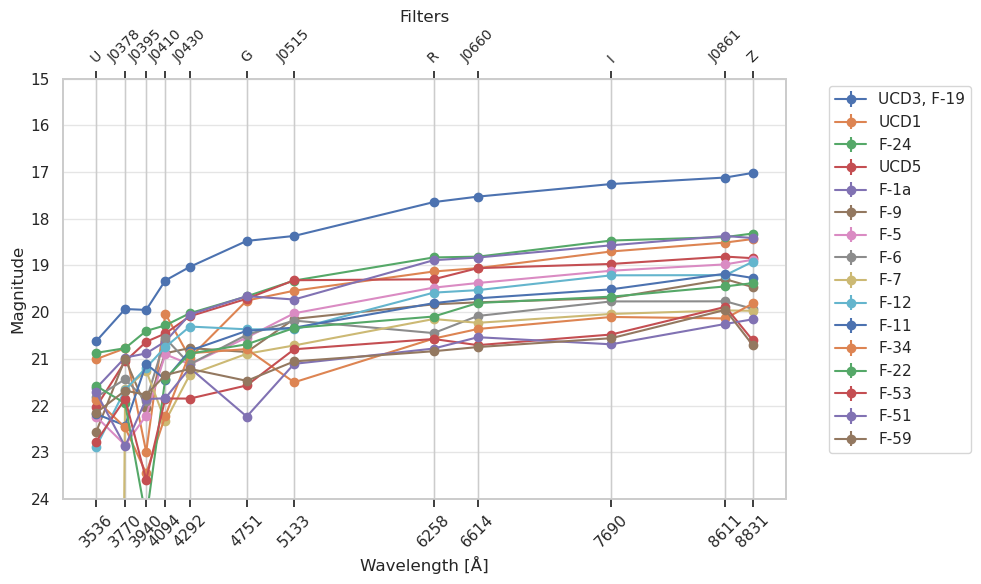
\includegraphics[width=\textwidth]{photo_specs/photospec_ucds.png}
        \caption{Fotoespectros das UCDs conhecidas em Fornax}
    \end{subfigure}
    \begin{subfigure}[b]{0.95\textwidth}
        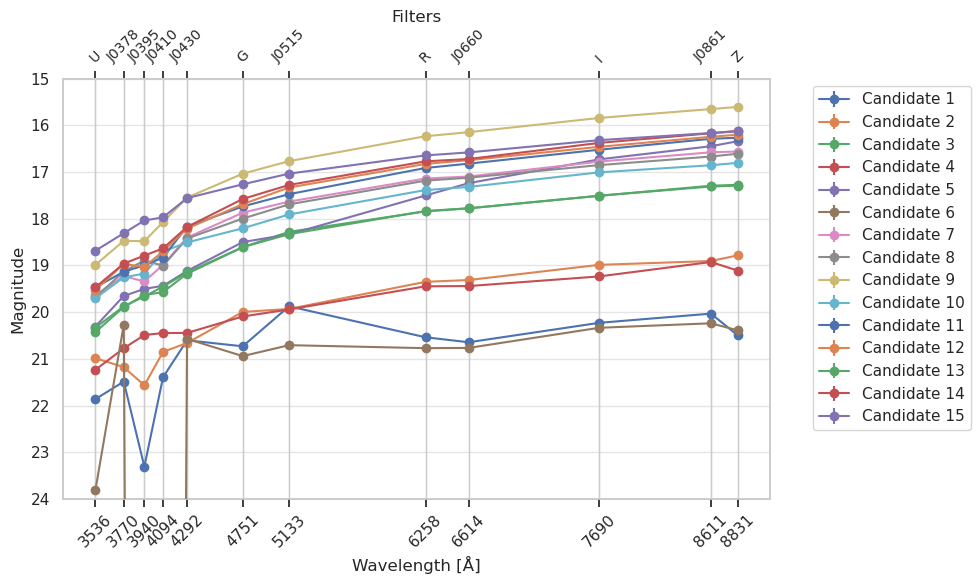
\includegraphics[width=\textwidth]{photo_specs/photospec_candidatas_sctarcut.png}
        \caption{Fotoespectros dos objetos selecionados da amostra de candidatas com corte estelar do GAIA DR3}
    \end{subfigure}
    \caption{Gráficos de fotoespectros sobrepostos das UCDs conhecidas em Fornax e dos objetos selecionados da amostra de candidatas com corte estelar do GAIA DR3.}
    \label{ucds_and_candiadates_star_cut_photospec}
\end{figure}

Na Figura \ref{ucds_and_candiadates_star_cut_photospec}, notamos que os objetos selecionados com o corte estelar do GAIA DR3 são, em média, mais brilhantes do que as UCDs conhecidas. Esse fato corrobora a ideia de que as possíveis galáxias mais brilhantes são mais facilmente classificadas corretamente pelo GAIA DR3. Observando as imagens dos objetos no Legacy Survey, notamos que parte dos objetos tem uma aparência mais extensa, e mesmo com os valores de \textit{FWHM} menores, apresentam parte de um disco ou braços espirais, e que podem ser objetos de fundo. Assim, escolhemos desses objetos aqueles que têm uma aparência mais pontual, com um critério visual, sem uma segunda componente extensa além do núcleo, selecionando 4 candidatas, semelhantes às UCDs conhecidas. Selecionamos também mais uma galáxia que, mesmo sendo um pouco mais extensa, está perto de uma galáxia massiva de Fornax, sendo interessante para estudos futuros.

Do restante da amostra de candidatas, com objetos mais fracos, que esperamos que o classificador estelar do GAIA DR3 tenha mais dificuldade em classificar, assim como as UCDs conhecidas mais fracas vistas na Figura \ref{distribuicao_fwhm_image_r_r_aper6_ucds_fornax}, esperamos também encontrar objetos interessantes. Para um critério mais objetivo, fizemos uso do outro classificador galáxia-estrela-quasar do S-PLUS DR4 (\textit{PROB\_GAL}, \textit{PROB\_STAR}, \textit{PROB\_QSO}) \citep{lili_classification}\footnote{Documentação S-PLUS Data Release 5: \url{https://splus.cloud/documentation/idr5}}. Ele oferece uma classificação levando em conta as bandas fotométricas do S-PLUS.
% e para uma faixa de objetos, ele apresenta discrepâncias em comparação com o GAIA DR3, principalmente para os objetos mais fracos. 

Selecionamos assim os objetos que foram classificados como galáxias pelo S-PLUS DR4, e que não foram selecionados pelo corte estelar do GAIA DR3 (\textit{PSS>0.5} + \textit{PROB\_GAL>0.5}). Dessa seleção foram retornados 12 objetos.

Tínhamos 217 objetos na nossa amostra de candidatas, dos quais selecionamos 5 interessantes pela classificação de galáxia do GAIA DR3, e mais 12 pela classificação de galáxia do S-PLUS DR4. Assim, temos um total de 17 objetos para a amostra final de candidatas a UCDs em Fornax.

\subsection{Seleção de candidatas com sinais de emissão} \label{subsec: candidatas_emissao}

Durante as etapas de aprimoramento na seleção de candidatas a UCDs, realizamos testes para identificar objetos com sinais de emissão. Na subseção \ref{subsection:candidatas_emissao}, explicamos a metodologia adotada, na qual, a partir de um conjunto inicial de candidatas selecionadas com base nos cortes do modelo de separação entre objetos extensos e compactos, realizamos uma inspeção visual de vários fotoespectros para identificar aqueles que apresentavam um pico evidente no filtro $J0660$.

Os resultados do pedido de observação dessas candidatas foram obtidos e, conforme apresentado na subseção \ref{subsection:resultado_espectros_emissao}, a análise dos dados confirmou que essa estratégia foi eficaz para identificar objetos com sinais de emissão. No entanto, nenhum dos seis objetos observados foi encontrado no redshift de Fornax.

Para as UCDs, não esperamos encontrar sinais de emissão. Assim, na primeira seleção de candidatas, adotamos apenas as probabilidades do modelo de separação entre objetos extensos e compactos, juntamente com os cortes definidos no início desta seção e os redshifts fotométricos.

No entanto, considerando que a subseleção de objetos compactos com características que evidenciam linhas de emissão sensíveis ao filtro $J0660$ se mostrou eficaz, incluímos um critério adicional que destaque esses objetos, se existirem na nossa amostra.

Na Figura \ref{ex_photospec_f600}, mostramos o fotoespectro de um dos exemplos das 6 candidatas que foram observadas com sinais de emissão. Notamos como o pico no filtro $J0660$ é evidente quando o comparamos com os dois filtros adjacentes, $r$ e $i$.

\begin{figure}[!ht]
    \begin{center}
    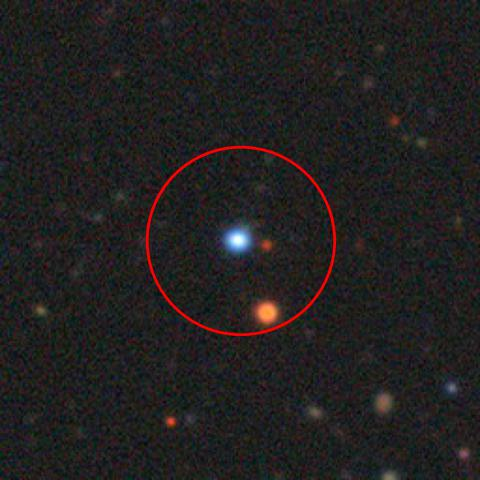
\includegraphics[width=0.85\columnwidth,angle=0]{photo_specs/Candidate_2.png}
    \caption[]{Imagem do \textit{Photo Spec}, criada pela Ferramenta Astroinspect \cite{astroinspect}, da \textit{Candidate\_2} da lista de candidatas da subseção \ref{subsection:candidatas_emissao} de objetos compactos com sinais de linhas de emissão no filtro $J0660$.}
    \label{ex_photospec_f600}
    \end{center}
\end{figure}

Para incluir esse critério, testamos criar uma seleção em cores com esses 3 filtros que destacassem esses objetos. A cor que iremos adotar é a diferença do filtro central, $J0660$, com a média dos filtros adjacentes, $r$ e $i$. Assim, esperamos que objetos com maiores picos tenham essa cor mais destoante. A cor adotada é a seguinte:

\begin{equation}
    \text{Color\_HAlpha} = J0660 - \frac{r + i}{2}
    \label{equantion_halpha_color}
\end{equation}

Demonstrando como essa cor utilizada pode destacar essa característica, criamos um gráfico contendo parte dos objetos da nossa amostra classificados como estrela ou galáxia, comparados com os 6 objetos com sinais de emissão que encontramos anteriormente. Na Figura \ref{color_halpha}, mostramos a distribuição dessa cor para esses objetos.

\begin{figure}[!ht]
    \begin{center}
    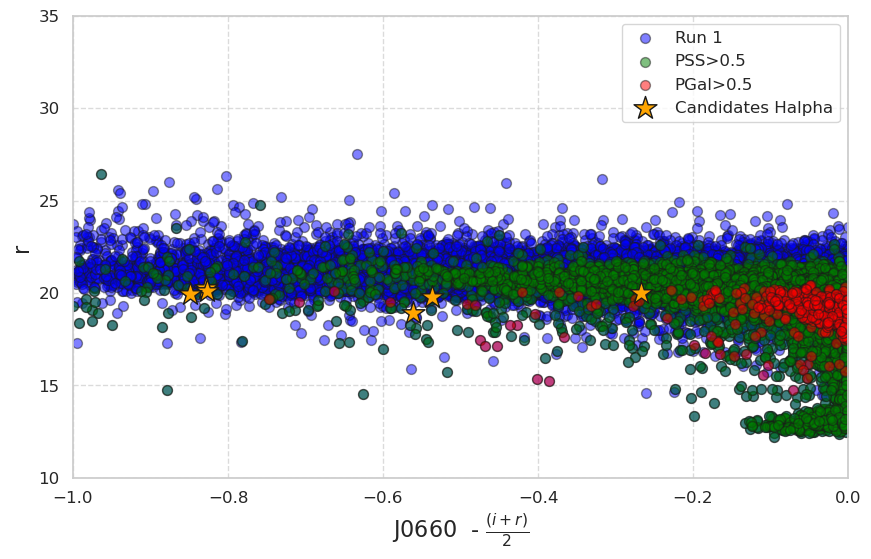
\includegraphics[width=1.\columnwidth,angle=0]{color_halpha.png}
    \caption[]{Gráfico da cor \text{Color\_HAlpha} em função da magnitude \textit{r\_APER\_6}. Pontos em azul são todos os dados da amostra de Fornax. Pontos em verde e vermelho são os objetos classificados como galáxias ou estrelas pelo GAIA DR3, respectivamente. Estrelas em amarelo são os 6 objetos com sinais de emissão que foram observados.}
    \label{color_halpha}
    \end{center}
\end{figure}

Pela Figura \ref{color_halpha}, notamos que os objetos com sinais de emissão se destacam a partir de um corte em \text{Color\_HAlpha}$\leq$-0.2. Vale ressaltar que, devido aos erros nos filtros e às diferenças entre as bandas $r$, $i$ e $J0660$, não necessariamente objetos com essa cor abaixo desse valor são representativos de terem um pico em $J0660$. Existem casos onde essa cor pode ser intensa devido a uma diferença brusca, de uma grande subida ou descida entre o filtro $i$ e $J0660$ ou $r$ e $J0660$, e não um pico propriamente dito. Então, mesmo sendo capaz de filtrar esses objetos, ainda precisamos avaliar visualmente os fotoespectros.

Da amostra de candidatas selecionadas, aplicamos esse corte para identificar objetos com sinais de emissão. Dos 217 objetos, obtivemos 4 objetos com essa cor abaixo do corte. Mostramos na Figura \ref{halpha_candidatas_final} o fotoespectro desses objetos.

\begin{figure}[!ht]
    \centering
    \captionsetup{justification=centering}
    \begin{subfigure}[b]{0.45\textwidth}
        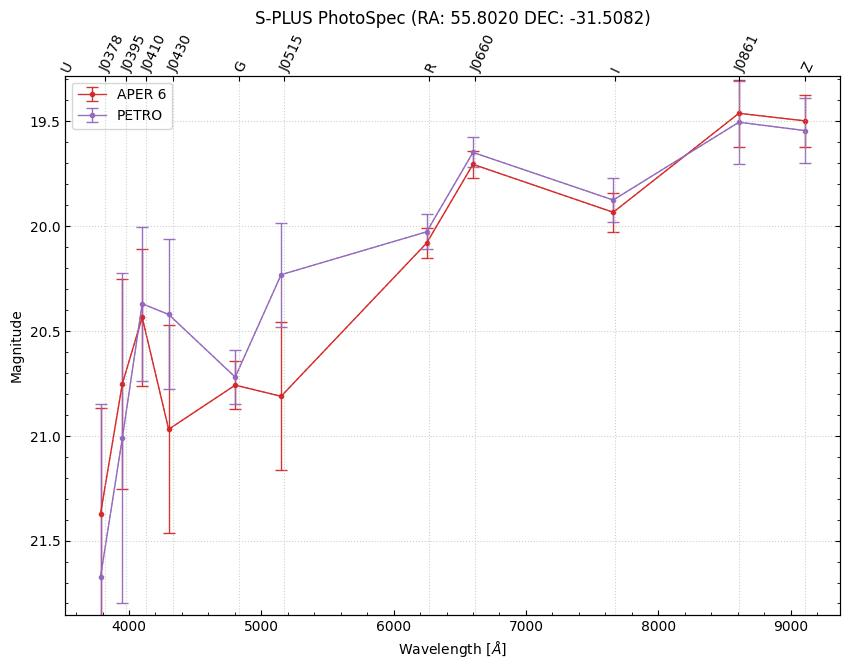
\includegraphics[width=\textwidth]{photo_specs/candidate_final/candidate_final_1.png}
        \caption{a)}
    \end{subfigure}
    \begin{subfigure}[b]{0.45\textwidth}
        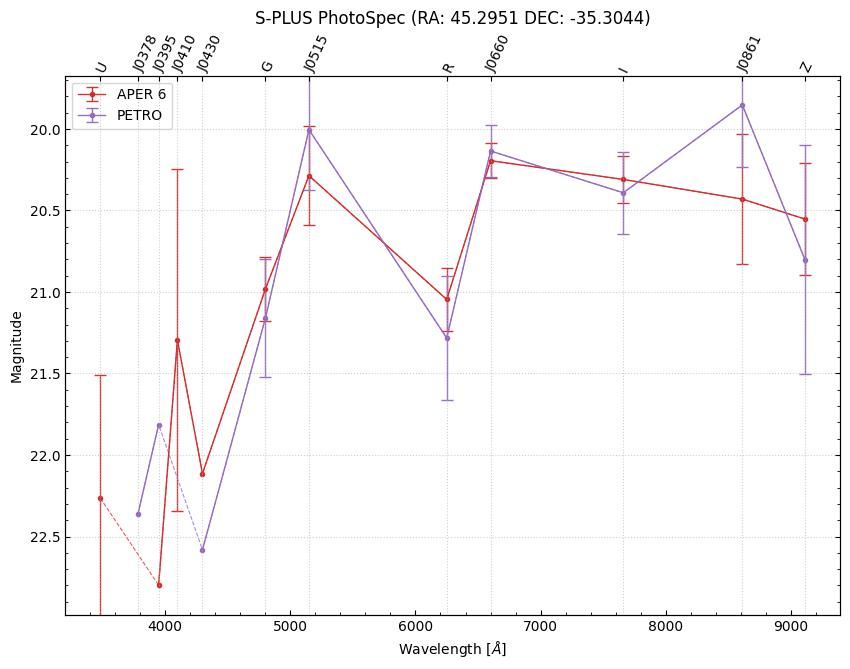
\includegraphics[width=\textwidth]{photo_specs/candidate_final/candidate_final_2.png}
        \caption{b)}
    \end{subfigure}
    \begin{subfigure}[b]{0.45\textwidth}
        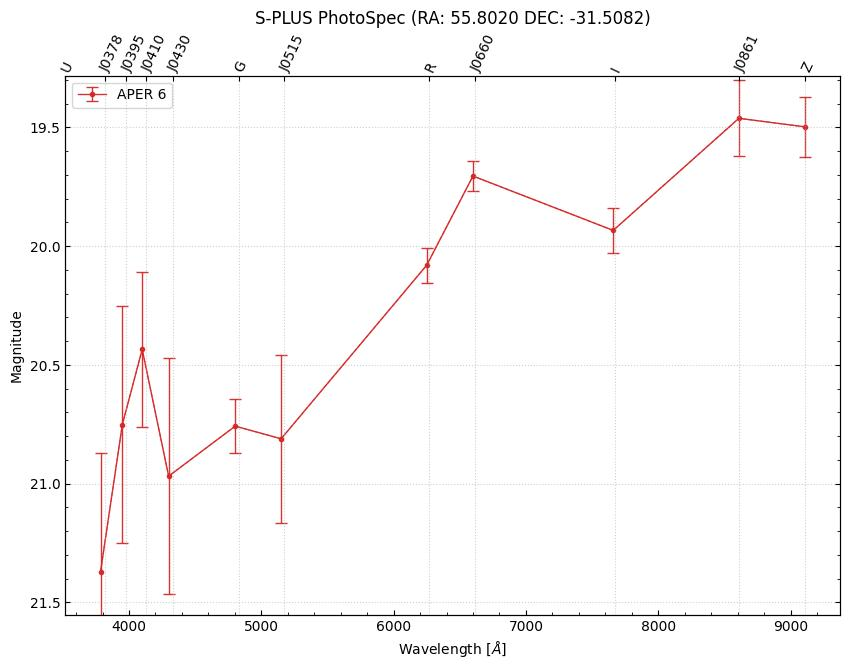
\includegraphics[width=\textwidth]{photo_specs/candidate_final/candidate_final_3.png}
        \caption{c)}
    \end{subfigure}
    \begin{subfigure}[b]{0.45\textwidth}
        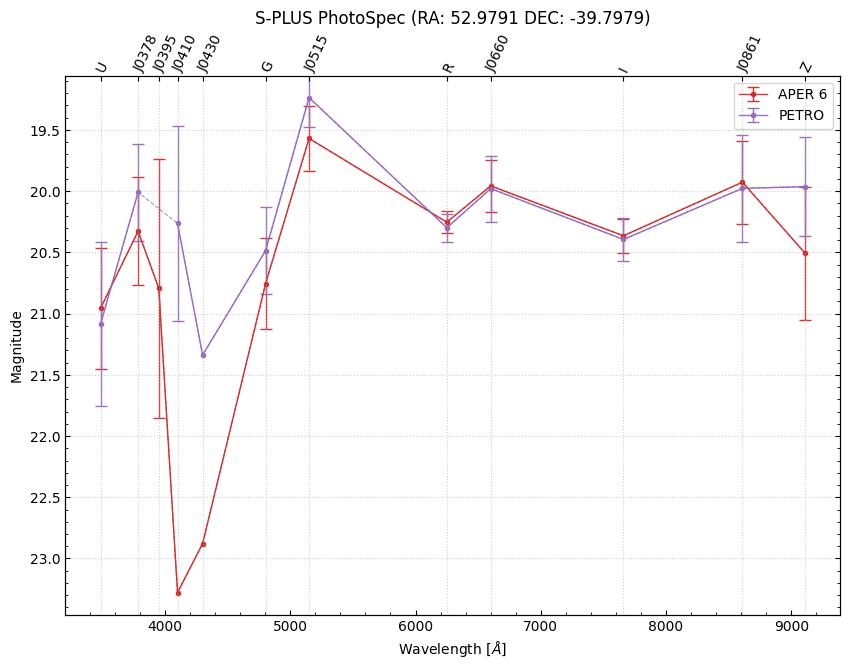
\includegraphics[width=\textwidth]{photo_specs/candidate_final/candidate_final_4.png}
        \caption{d)}
    \end{subfigure}
    \caption{Imagens dos \textit{Photo Spec}, criadas pela Ferramenta Astroinspect \cite{astroinspect}, com corte na cor criada pela equação \ref{equantion_halpha_color}, aplicando um corte abaixo de -0.3 na lista de candidatas finais a objetos compactos de Fornax da seção \ref{cap:selecao_candidatas}.}
    \label{halpha_candidatas_final}
\end{figure}

\section{Análise das candidatas}\label{sec:analise_candidatas}

Selecionamos 17 objetos para a amostra final de candidatas a UCDs da seção \ref{cap:selecao_candidatas} mais 4 objetos com possíveis sinais de emissão da subseção \ref{subsec: candidatas_emissao}, totalizando 21 objetos.

Utilizando o catálogo de Fornax proveniente do projeto S-PLUS Fornax \citep{castelli2024splusfornaxprojectsfp}, com a fotometria apresentada por \citep{haack2024splusfornaxprojectsfp}, obtivemos uma amostra de galáxias conhecidas, classificadas morfologicamente. Com base nisso, realizamos uma análise das candidatas selecionadas, comparando-as com as galáxias conhecidas. Identificamos, em diversos conjuntos de parâmetros, tanto a localização das UCDs reais quanto a posição das nossas candidatas.

Selecionamos as categorias morfológicas de galáxias mais relevantes com as maiores quantidades de objetos para comparação. Dentre elas, temos as galáxias anãs elípticas, nucleadas e não nucleadas, junto das irregulares. Outros tipos importantes incluem as LSB (Low Surface Brightness) e as galáxias espirais.

Investigamos aqui como as UCDs e galáxias conhecidas pela morfologia se distribuem em diferentes espaços de parâmetros, especialmente aqueles que representam a morfologia dos objetos compactos. Um dos parâmetros analisados foi o brilho superficial médio, aqui usado na banda $r$, que é uma medida da densidade superficial de luminosidade média de um objeto. Ele foi calculado a partir da magnitude aparente e do raio efetivo do objeto. Usamos a informação do \textit{PETRO\_RADIUS}, que está em unidades dos parâmetros \textit{A} e \textit{B}, do SExtractor, para calcular o raio do objeto. A partir disso, calculamos o brilho superficial médio, que é a magnitude aparente menos 2.5 vezes o logaritmo do raio efetivo ao quadrado, convertido para unidades de arcsec$^2$. A equação para o cálculo do brilho superficial médio é a seguinte:

\begin{equation}
    \mu_{\text{medio}} = \text{mag\_aparente} - 2.5 \times \log_{10}(\pi \times A \times B \times 0.55 \times \text{PETRO\_RADIUS})
    \label{equation_sb}
\end{equation}

Na Figura \ref{sb_r_ucds_galaxias}, mostramos a distribuição do brilho superficial médio na banda $r$ para as UCDs conhecidas e as galáxias morfologicamente classificadas, juntamente com as candidatas selecionadas.

\begin{figure}[!ht]
    \begin{center}
    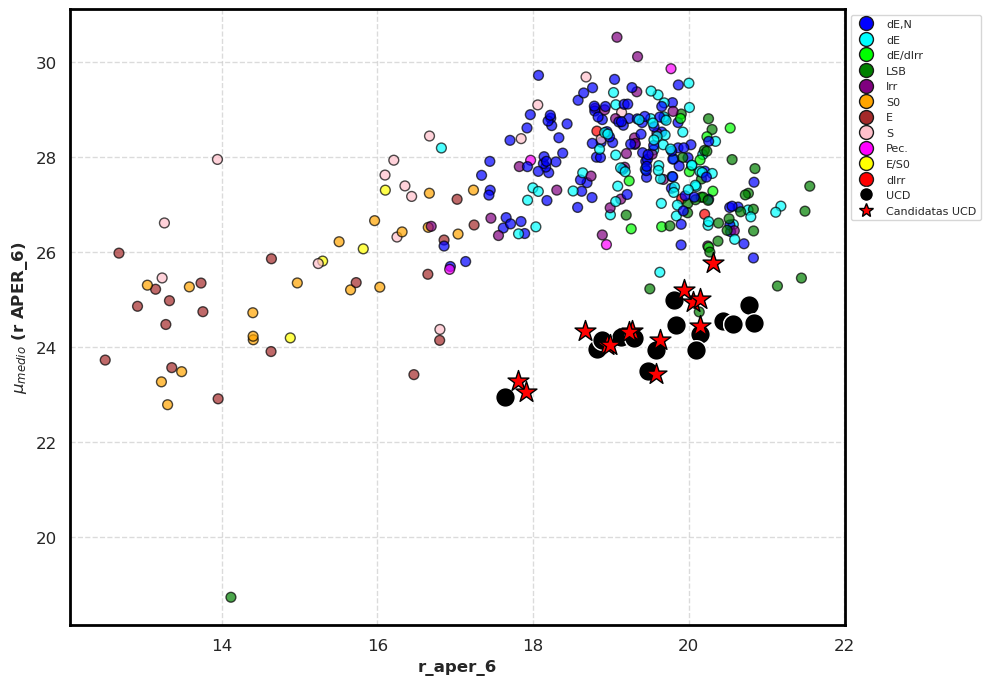
\includegraphics[width=1.\columnwidth,angle=0]{sb_r_ucds_galaxias.png}
    \caption[]{Gráfico da magnitude superficial média na banda $r$ em função da magnitude aparente na banda $r$ para as UCDs conhecidas, as galáxias morfologicamente classificadas e as candidatas selecionadas.}
    \label{sb_r_ucds_galaxias}
    \end{center}
\end{figure}

A Figura \ref{sb_r_ucds_galaxias} mostra que, para parte das galáxias com morfologia conhecida apresentadas, elas seguem uma distribuição em cauda para o brilho superficial médio na banda $r$, em função da magnitude aparente na banda $r$. Para as UCDs conhecidas e as candidatas, elas estão localizadas na parte superior, em um segundo conjunto de curva. Esse fato mostra que, para um mesmo brilho superficial médio, as UCDs e as candidatas são mais brilhantes que as galáxias de morfologia apresentada, que são mais extensas. Em outras palavras, para o mesmo intervalo de magnitude (ou luminosidade), as UCDs têm raios efetivos muito menores do que galáxias típicas e, portanto, exibem brilhos superficiais mais elevados.

Tanto para os cenários previstos de formação das UCDs como núcleos expostos de galáxias anãs que foram despojadas de suas camadas externas por interações gravitacionais em aglomerados, quanto para aqueles de formação a partir de aglomerados estelares massivos, o resultado são objetos com alta densidade estelar e raios efetivos pequenos, o que gera um brilho superficial alto.

Nesse tipo de diagrama, quando comparado com as galáxias de morfologia “convencional” (elípticas, espirais, etc.), essa diferença estrutural dos dois tipos é evidenciada: as UCDs ocupam uma região “compacta e luminosa” para seu tamanho, enquanto as galáxias seguem uma correlação mais “espalhada” entre luminosidade e tamanho/brilho superficial.

Na Figura \ref{r_aper_6_mu_max} e \ref{r_aper_6_kron_radius}, temos os parâmetros \textit{MU\_MAX} e \textit{KRON\_RADIUS}, respectivamente, ambos em função da magnitude aparente na banda $r$. O \textit{MU\_MAX} representa o pico de brilho superficial do objeto, medido em magnitudes por arcsegundo quadrado, indicando o quão brilhante é a região mais intensa do objeto em comparação com o fundo. Já o \textit{KRON\_RADIUS} (raio de Kron) é o raio principal de medição definido pelo SExtractor para estimar a magnitude total. Ele é calculado com base na distribuição de luz do objeto, usando o fluxo integrado ao longo de elipses que seguem o perfil de brilho do mesmo objeto.

Em ambas as figuras, observamos que as candidatas se localizam em regiões mais próximas das UCDs conhecidas do que das demais galáxias com morfologia apresentada. Na Figura \ref{r_aper_6_mu_max}, vemos que elas seguem uma segunda curva abaixo das galáxias mais extensas. Já para a Figura \ref{r_aper_6_kron_radius}, vemos que, conforme os objetos ficam mais fracos, o raio de Kron aumenta. Quando um objeto é mais extenso ou tem a luz distribuída de forma difusa, a ferramenta precisa usar um raio maior para abranger boa parte do fluxo total. Em outras palavras, objetos mais fracos (mas espalhados em área maior) resultam em um Kron Radius maior, pois o algoritmo “enxerga” a luz se estendendo além de um núcleo compacto. Já objetos brilhantes e concentrados apresentam Kron Radius menor, pois a maior parte do fluxo está contida numa região pequena. Ainda assim, notamos que as candidatas selecionadas e UCDs conhecidas têm a mesma tendência, porém agrupadas em uma região mais abaixo do gráfico.

\begin{figure}[!ht]
    \begin{center}
    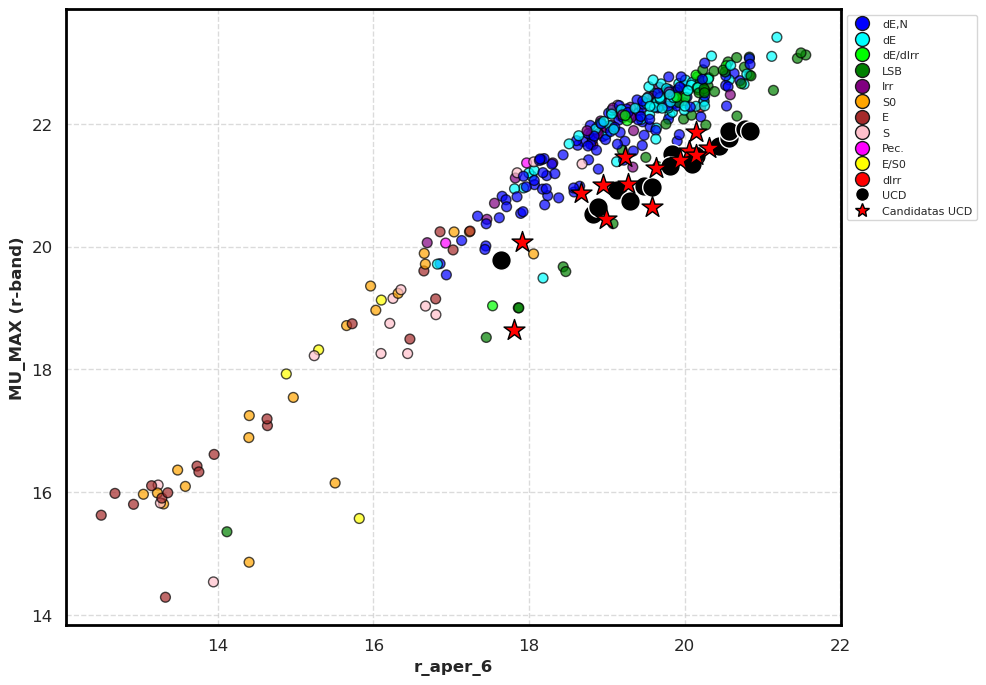
\includegraphics[width=1.\columnwidth,angle=0]{r_aper_6_mu_max.png}
    \caption[]{Gráfico do parâmetro \textit{MU\_MAX} em função da magnitude aparente na banda $r$ para as UCDs conhecidas, as galáxias morfologicamente classificadas e as candidatas selecionadas.}
    \label{r_aper_6_mu_max}
    \end{center}
\end{figure}


\begin{figure}[!ht]
    \begin{center}
    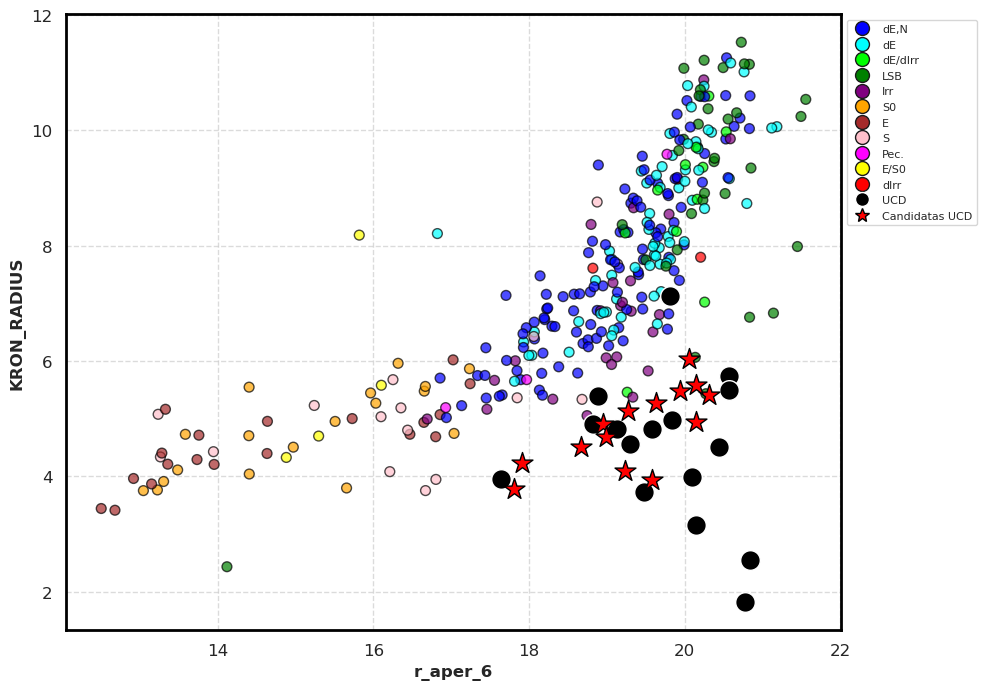
\includegraphics[width=1.\columnwidth,angle=0]{r_aper_6_kron_radius.png}
    \caption[]{Gráfico do parâmetro \textit{KRON\_RADIUS} em função da magnitude aparente na banda $r$ para as UCDs conhecidas, as galáxias morfologicamente classificadas e as candidatas selecionadas.}
    \label{r_aper_6_kron_radius}
    \end{center}
\end{figure}


\section{Candidatas para espectroscopia}\label{sec:candidatas_espectroscopia}

Nesta seção, discutiremos os objetos selecionados para espectroscopia ao longo do projeto. Dando sequência a um projeto anterior de iniciação científica, foram selecionadas 18 candidatas a UCDs. Na época do projeto, foi submetido um pedido de tempo ao telescópio Gemini Sul para observação espectroscópica com o GMOS. Até o momento, 14 dessas candidatas foram observadas. Como parte do início deste projeto, foi feita a aquisição desses objetos para análise dos espectros.

Na Tabela \ref{candidatas_espectroscopia_1}, temos a lista dessas candidatas observadas, com suas respectivas coordenadas. Utilizando o Legacy Survey Sky Browser\footnote{Legacy Survey Sky Browser}, apresentamos na Figura \ref{candidatas_espectroscopia_1_img} as imagens desses objetos.

\begin{table}[!ht]
    \centering
    \caption{Conjunto de candidatas a UCDs observadas com o GMOS no telescópio Gemini Sul, selecionadas de um projeto anterior. A coluna $OBJ_{name}$ é o nome interno da candidata utilizado no pedido de tempo do Gemini.} 
    \begin{tabular}{lcc}
        \toprule
        $OBJ_{name}$ & RA     & DEC     \\
        \midrule
        UCG01     & 47,708 & -34,157 \\
        UCG02     & 47,960 & -33,174 \\
        UCG03     & 49,910 & -31,523 \\
        UCG04     & 53,753 & -37,155 \\
        UCG05     & 53,820 & -35,837 \\
        UCG06     & 54,115 & -36,845 \\
        UCG07     & 54,214 & -36,814 \\
        UCG08     & 54,912 & -35,439 \\
        UCG09     & 55,010 & -35,535 \\
        UCG10     & 55,056 & -37,895 \\
        UCG11     & 55,211 & -38,048 \\
        UCG12     & 55,315 & -37,020 \\
        UCG13     & 55,333 & -36,653 \\
        UCG14     & 55,673 & -36,541 \\
        UCG15     & 57,272 & -35,515 \\
        UCG16     & 57,468 & -34,663 \\
        UCG17     & 58,035 & -37,111 \\
        UCG18     & 58,083 & -36,298 \\
        \bottomrule
    \end{tabular}
    \label{candidatas_espectroscopia_1}
\end{table}


\begin{figure}[!ht]
    \centering
    \captionsetup{justification=centering}
    \begin{subfigure}[b]{0.22\textwidth}
        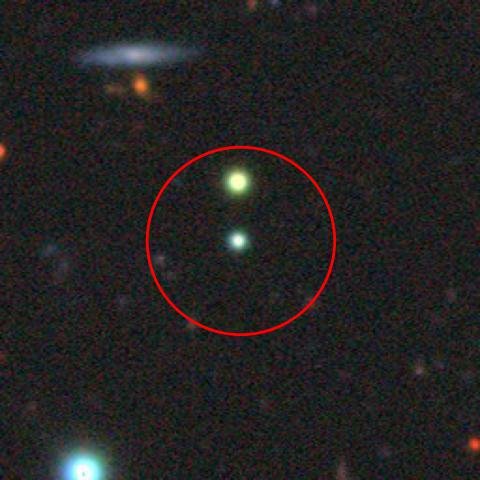
\includegraphics[width=\textwidth]{proposatal_candidatas_1/UCG01.png}
        \caption{UCG01}
    \end{subfigure}
    \begin{subfigure}[b]{0.22\textwidth}
        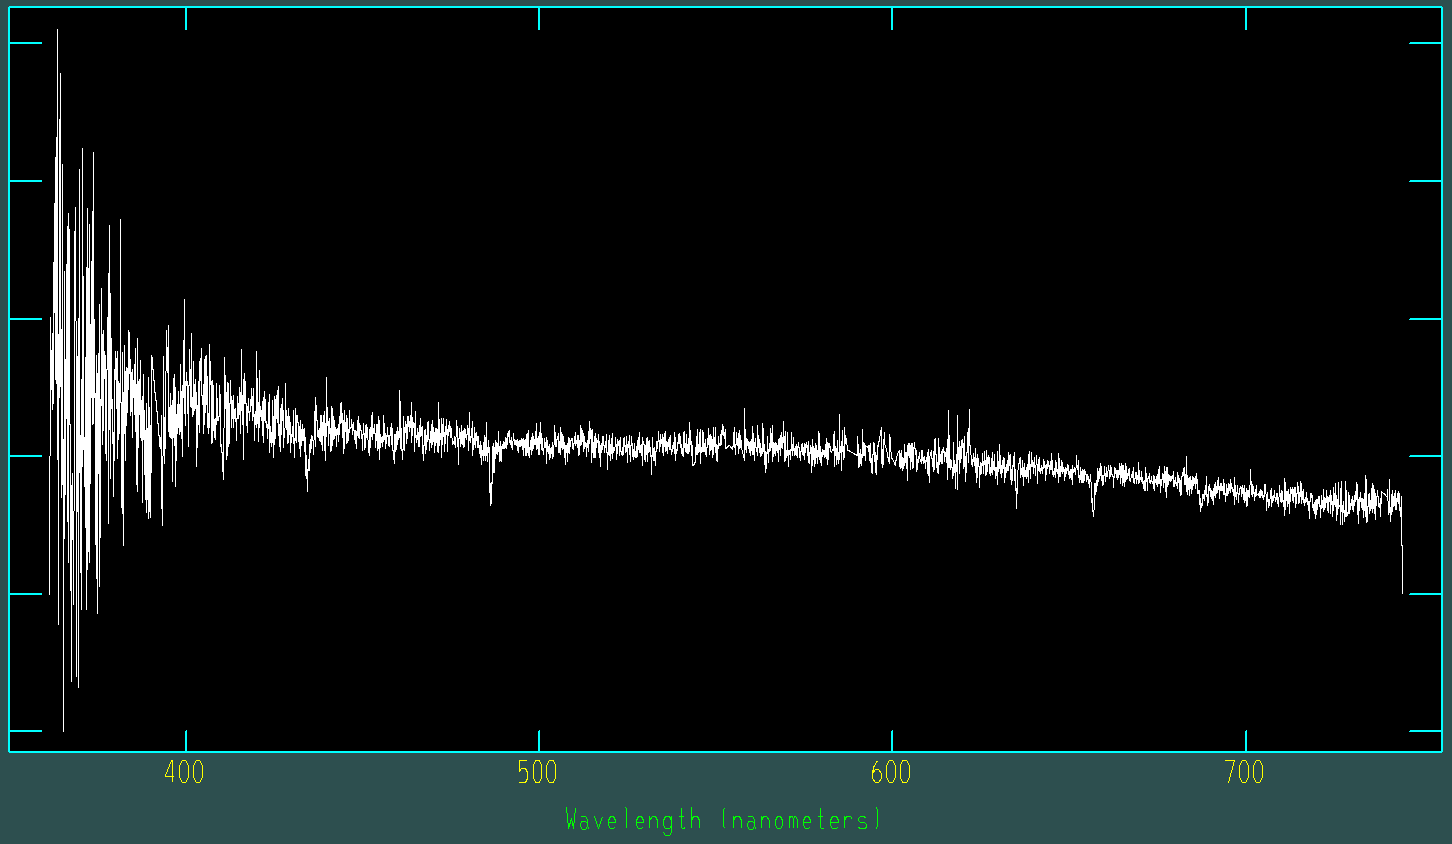
\includegraphics[width=\textwidth]{proposatal_candidatas_1/UCG02.png}
        \caption{UCG02}
    \end{subfigure}
    \begin{subfigure}[b]{0.22\textwidth}
        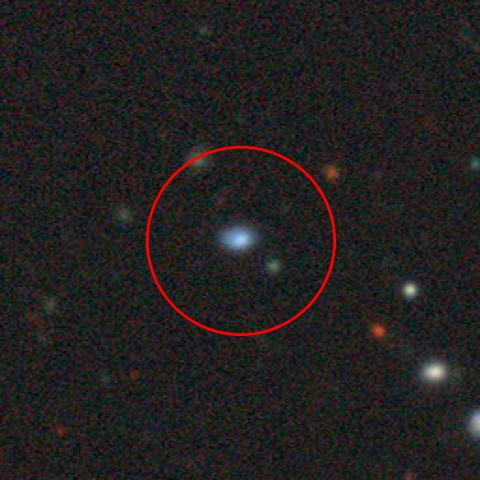
\includegraphics[width=\textwidth]{proposatal_candidatas_1/UCG03.jpg}
        \caption{UCG03}
    \end{subfigure}
    \begin{subfigure}[b]{0.22\textwidth}
        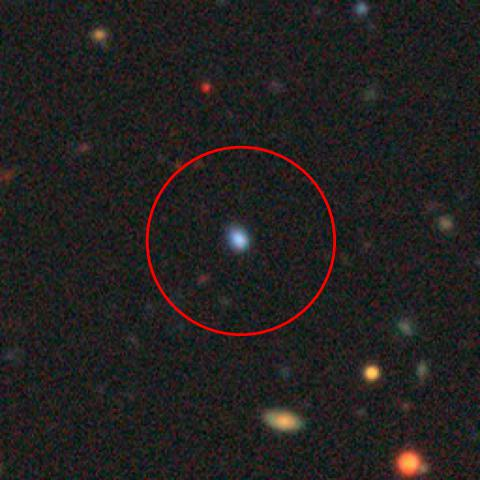
\includegraphics[width=\textwidth]{proposatal_candidatas_1/UCG04.jpg}
        \caption{UCG04}
    \end{subfigure}
    \begin{subfigure}[b]{0.22\textwidth}
        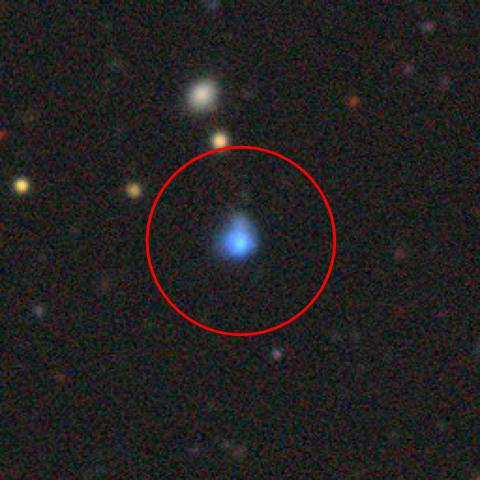
\includegraphics[width=\textwidth]{proposatal_candidatas_1/UCG05.jpg}
        \caption{UCG05}
    \end{subfigure}
    \begin{subfigure}[b]{0.22\textwidth}
        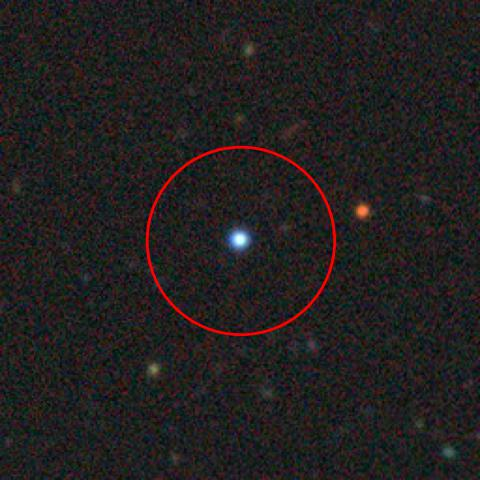
\includegraphics[width=\textwidth]{proposatal_candidatas_1/UCG06.jpg}
        \caption{UCG06}
    \end{subfigure}
    \begin{subfigure}[b]{0.22\textwidth}
        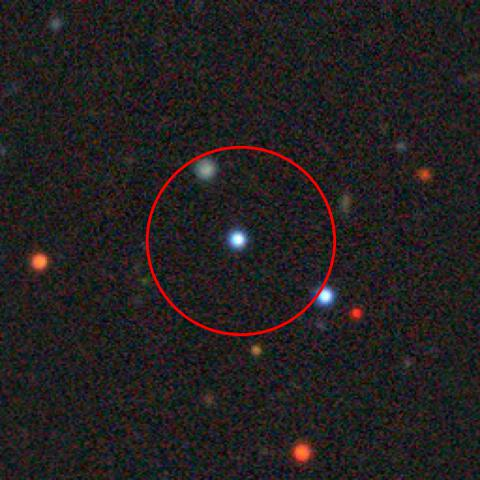
\includegraphics[width=\textwidth]{proposatal_candidatas_1/UCG07.jpg}
        \caption{UCG07}
    \end{subfigure}
    \begin{subfigure}[b]{0.22\textwidth}
        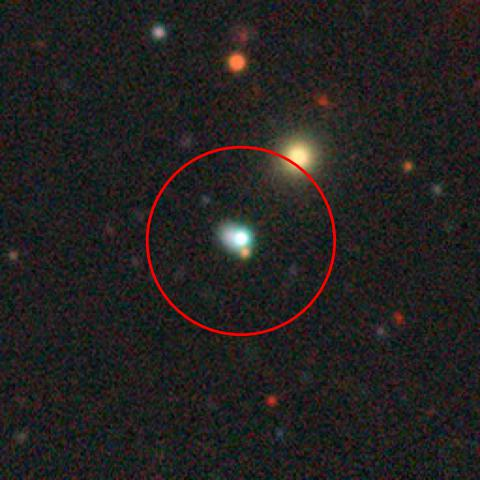
\includegraphics[width=\textwidth]{proposatal_candidatas_1/UCG08.jpg}
        \caption{UCG08}
    \end{subfigure}
    \begin{subfigure}[b]{0.22\textwidth}
        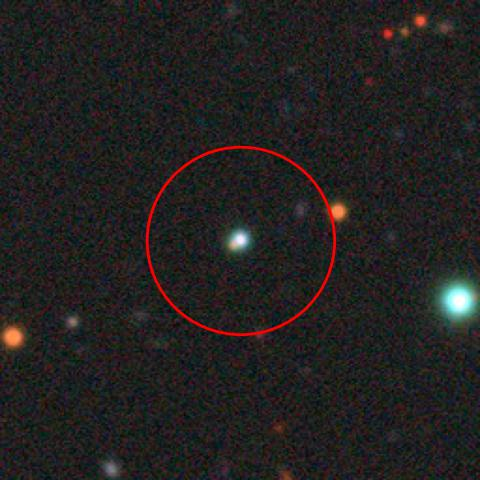
\includegraphics[width=\textwidth]{proposatal_candidatas_1/UCG09.jpg}
        \caption{UCG09}
    \end{subfigure}
    \begin{subfigure}[b]{0.22\textwidth}
        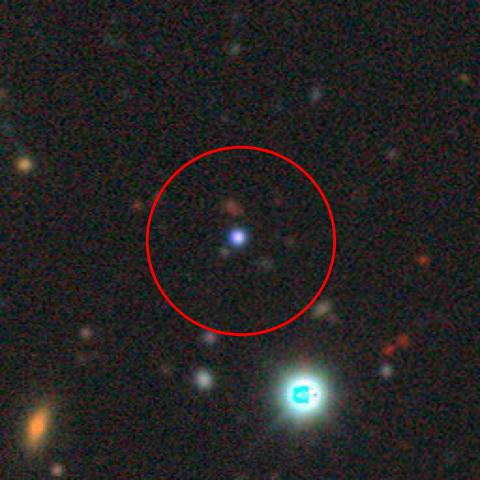
\includegraphics[width=\textwidth]{proposatal_candidatas_1/UCG10.jpg}
        \caption{UCG10}
    \end{subfigure}
    \begin{subfigure}[b]{0.22\textwidth}
        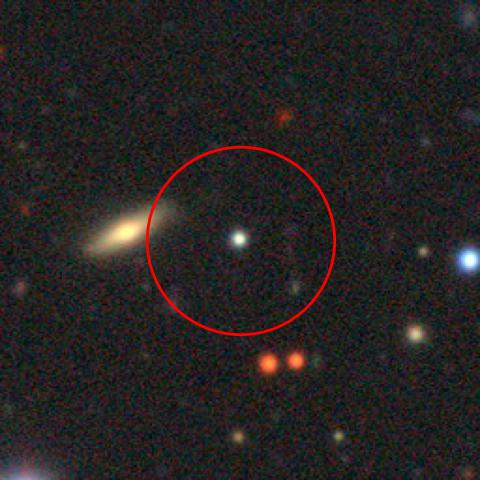
\includegraphics[width=\textwidth]{proposatal_candidatas_1/UCG11.jpg}
        \caption{UCG11}
    \end{subfigure}
    \begin{subfigure}[b]{0.22\textwidth}
        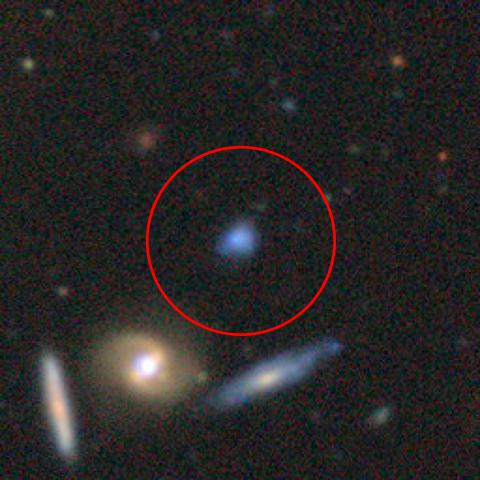
\includegraphics[width=\textwidth]{proposatal_candidatas_1/UCG12.jpg}
        \caption{UCG12}
    \end{subfigure}
    \begin{subfigure}[b]{0.22\textwidth}
        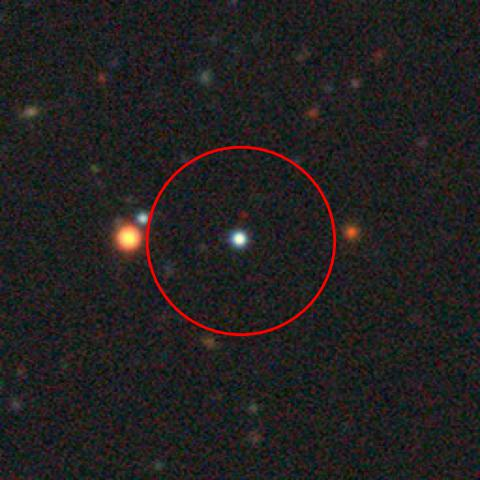
\includegraphics[width=\textwidth]{proposatal_candidatas_1/UCG13.jpg}
        \caption{UCG13}
    \end{subfigure}
    \begin{subfigure}[b]{0.22\textwidth}
        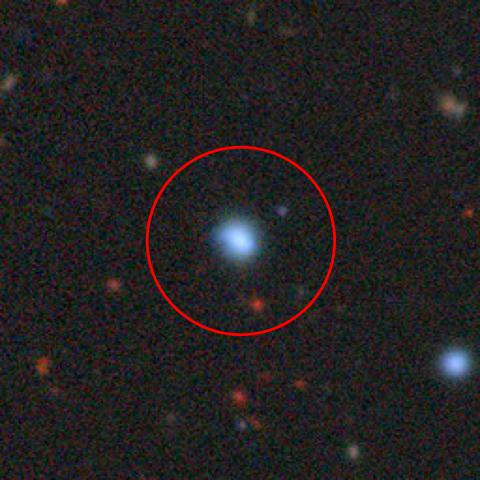
\includegraphics[width=\textwidth]{proposatal_candidatas_1/UCG14.jpg}
        \caption{UCG14}
    \end{subfigure}
    \begin{subfigure}[b]{0.22\textwidth}
        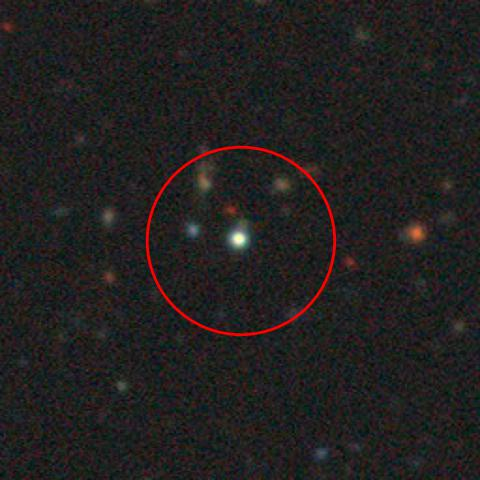
\includegraphics[width=\textwidth]{proposatal_candidatas_1/UCG15.jpg}
        \caption{UCG15}
    \end{subfigure}
    \begin{subfigure}[b]{0.22\textwidth}
        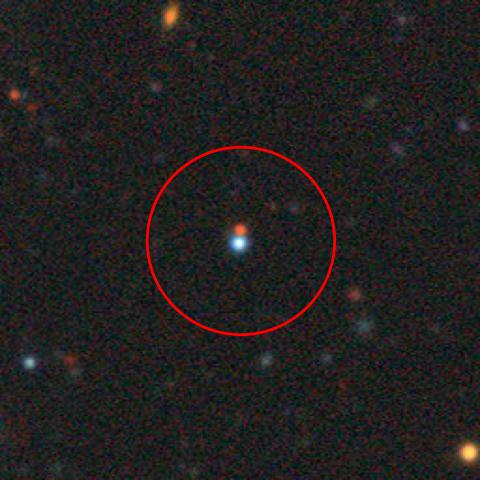
\includegraphics[width=\textwidth]{proposatal_candidatas_1/UCG16.jpg}
        \caption{UCG16}
    \end{subfigure}
    \begin{subfigure}[b]{0.22\textwidth}
        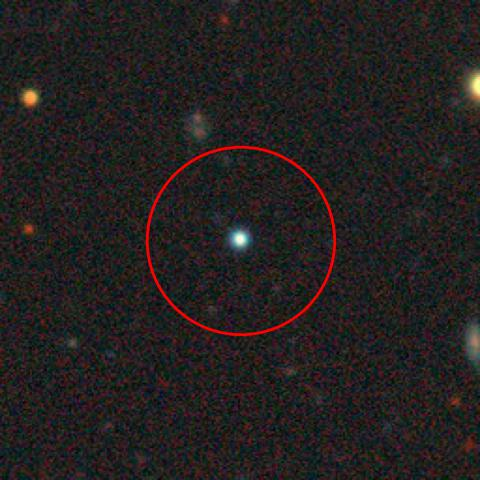
\includegraphics[width=\textwidth]{proposatal_candidatas_1/UCG17.jpg}
        \caption{UCG17}
    \end{subfigure}
    \begin{subfigure}[b]{0.22\textwidth}
        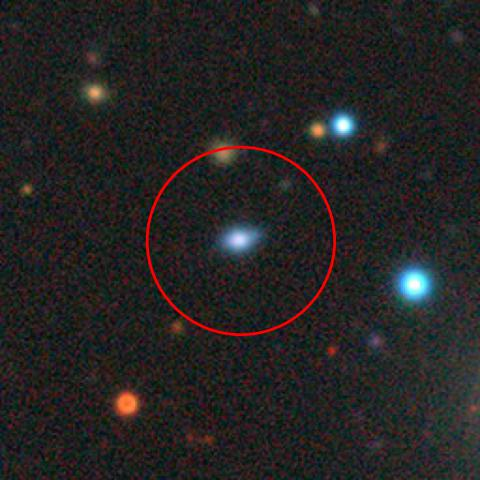
\includegraphics[width=\textwidth]{proposatal_candidatas_1/UCG18.jpg}
        \caption{UCG18}
    \end{subfigure}
    \caption{Imagens das candidatas a UCDs observadas com o GMOS no telescópio Gemini Sul, selecionadas de um projeto anterior. Imagens obtidas pelo Legacy Survey. Os nomes correspondem ao mesmo nome do objeto da Tabela \ref{candidatas_espectroscopia_1}.}
    \label{candidatas_espectroscopia_1_img}
\end{figure}


\subsection{Candidatas com sinais de linhas de emisssão}\label{subsection:candidatas_emissao}

A partir da lista de candidatas explicadas na seção \ref{cap:selecao_candidatas}, selecionamos algumas com características interessantes para um pedido de tempo de espectroscopia. Utilizando a ferramenta Astroinspect \cite{astroinspect}, podemos fornecer uma tabela de objetos, e ela nos retorna, por exemplo, o \textit{Photo Spec}, isto é, uma imagem do espectro do objeto a partir das medições dos filtros fotométricos do S-PLUS.

Nosso objetivo inicial foi, dentro da amostra de candidatas, encontrar aquelas cujo \textit{Photo Spec} apresentassem um salto nas medições do filtro $J0660$. Esse salto poderia indicar a presença de linhas de emissão de H$\alpha$ (esperadas para esse filtro em repouso), o que seria um indicativo de que, dado o redshift baixo de Fornax, poderíamos estar observando objetos dentro do intervalo de redshifts compatíveis com o aglomerado. Ou seja, se existir algum objeto com emissões em H$\alpha$ em Fornax, é esperado observar um salto no filtro $J0660$, mesmo que levemente deslocado em relação ao filtro em repouso.

Das candidatas retiradas após os cortes adotados na seção \ref{cap:selecao_candidatas}, selecionamos 6 objetos com sinais de linhas de emissão. Na Figura \ref{photo_spec_candidatas}, apresentamos os \textit{Photo Spec} desses objetos, criados com a ferramenta Astroinspect.

\begin{figure}[!ht]
    \centering
    \captionsetup{justification=centering}
    \begin{subfigure}[b]{0.3\textwidth}
        \includegraphics[width=\textwidth]{photo_specs/Candidate_1.png}
        \caption{Candidate\_1}
    \end{subfigure}
    \begin{subfigure}[b]{0.3\textwidth}
        \includegraphics[width=\textwidth]{photo_specs/Candidate_2.png}
        \caption{Candidate\_2}
    \end{subfigure}
    \begin{subfigure}[b]{0.3\textwidth}
        \includegraphics[width=\textwidth]{photo_specs/Candidate_3.png}
        \caption{Candidate\_3}
    \end{subfigure}
    \begin{subfigure}[b]{0.3\textwidth}
        \includegraphics[width=\textwidth]{photo_specs/Candidate_4.png}
        \caption{Candidate\_4}
    \end{subfigure}
    \begin{subfigure}[b]{0.3\textwidth}
        \includegraphics[width=\textwidth]{photo_specs/Candidate_5.png}
        \caption{Candidate\_5}
    \end{subfigure}
    \begin{subfigure}[b]{0.3\textwidth}
        \includegraphics[width=\textwidth]{photo_specs/Candidate_6.png}
        \caption{Candidate\_6}
    \end{subfigure}
    \caption{Imagens dos \textit{Photo Spec}, criadas pela Ferramenta Astroinspect \cite{astroinspect}, das candidatas a objetos compactos com sinais de linhas de emissão no filtro J0660. Os nomes correspondem ao nome interno usado para o pedido de tempo de observação espectroscópica no Gemini.}
    \label{photo_spec_candidatas}
\end{figure}

Observamos na Figura \ref{photo_spec_candidatas} que os objetos apresentam sinais de linhas de emissão no filtro J0660, conforme comentado. Dessa forma, esses objetos foram selecionados para a observação espectroscópica no Gemini Sul. Na Figura \ref{candidatas_espectroscopia_2_img}, apresentamos as imagens desses objetos.

\begin{figure}[!ht]
    \centering
    \captionsetup{justification=centering}
    \begin{subfigure}[b]{0.25\textwidth}
        \includegraphics[width=\textwidth]{proposatal_candidatas_2/Candidate_1.png}
        \caption{Candidate\_1}
    \end{subfigure}
    \begin{subfigure}[b]{0.25\textwidth}
        \includegraphics[width=\textwidth]{proposatal_candidatas_2/Candidate_2.png}
        \caption{Candidate\_2}
    \end{subfigure}
    \begin{subfigure}[b]{0.25\textwidth}
        \includegraphics[width=\textwidth]{proposatal_candidatas_2/Candidate_3.png}
        \caption{Candidate\_3}
    \end{subfigure}
    \begin{subfigure}[b]{0.25\textwidth}
        \includegraphics[width=\textwidth]{proposatal_candidatas_2/Candidate_4.png}
        \caption{Candidate\_4}
    \end{subfigure}
    \begin{subfigure}[b]{0.25\textwidth}
        \includegraphics[width=\textwidth]{proposatal_candidatas_2/Candidate_5.png}
        \caption{Candidate\_5}
    \end{subfigure}
    \begin{subfigure}[b]{0.25\textwidth}
        \includegraphics[width=\textwidth]{proposatal_candidatas_2/Candidate_6.png}
        \caption{Candidate\_6}
    \end{subfigure}
    \caption{Imagens das candidatas a objetos compactos com sinais de linhas de emissão no filtro J0660. Imagens obtidas pelo Legacy Survey. Os nomes correspondem à mesma lista de \textit{Photo Spec} da Figura \ref{photo_spec_candidatas}.}
    \label{candidatas_espectroscopia_2_img}
\end{figure}

\section{Redução dos Espectros}\label{sec:reducao_espectros}

Os dados espectroscópicos do telescópio Gemini não passam por um tratamento inicial, então é necessário um pré-processamento. Esse passo é crucial para limpar as imagens de sinais indesejados, removendo ruídos dos instrumentos e convertendo os espectros bidimensionais em unidimensionais para análise.

Fizemos a redução dos dados usando o Software de Redução de Dados DRAGONS (Data Reduction for Astronomy with Gemini Observatory's Node System) \cite{dragons_python}. Esse software permite reduzir os dados tanto pela linha de comando quanto por meio de uma API em Python. Optamos pela API em Python para tornar o processo mais eficiente e agilizar a geração dos espectros unidimensionais (1D) e bidimensionais (2D) para cada objeto.

\textbf{Seleção de Dados}

O primeiro passo para a redução é a seleção dos dados que serão usados, como os arquivos de \textit{bias}, \textit{flats}, \textit{arcs}, estrelas padrão (\textit{standard star}) e os dados científicos. Utilizamos a função \verb|dataselect.select_data|, que permite filtrar os arquivos por algumas características específicas, como o tipo de detector e o objeto observado.

\textbf{Redução do \textit{Bias}}

A etapa inicial da redução é a correção de \textit{bias}, onde os arquivos são processados para remover o sinal eletrônico residual presente nas imagens. Utilizando a função \verb|Reduce|, criamos dois conjuntos de arquivos de \textit{bias}: um para as estrelas padrão e outro para os dados científicos. Essa correção visa garantir que o sinal obtido nas observações não seja contaminado por ruídos instrumentais.

\textbf{Redução dos \textit{Flats}}

Após a correção de \textit{bias}, processamos as imagens de \textit{flat-field}, que corrigem variações na resposta do detector em diferentes regiões do campo de visão. Os arquivos de \textit{flats} são selecionados e processados novamente com a função \verb|Reduce|, assegurando a uniformidade na resposta do detector em todas as partes do espectro.

\textbf{Redução dos \textit{Arcs}}

Na sequência, realizamos a redução dos arquivos de \textit{arcs}, que contêm linhas de emissão conhecidas utilizadas para calibrar a escala de comprimento de onda dos espectros. A função \verb|Reduce| é aplicada para processar os \textit{arcs}, ajustando as linhas de emissão observadas ao modelo teórico e garantindo que os comprimentos de onda sejam medidos com precisão.

\textbf{Redução da Estrela Padrão}

Para a redução da estrela padrão (\textit{standard star}), também utilizamos a função \verb|Reduce| para processar essas observações, gerando um espectro calibrado em fluxo, que serve como referência para a normalização dos espectros dos objetos científicos. O espectro resultante é plotado e analisado para verificar a qualidade da calibração.

\textbf{Redução dos Dados Científicos}

Finalmente, os dados científicos são reduzidos aplicando todas as correções anteriores (\textit{bias}, \textit{flat}, \textit{arc}) aos dados de observação dos objetos de interesse, novamente utilizando a função \verb|Reduce|. Esse processo resulta na geração dos espectros unidimensionais (\textit{1D}) e bidimensionais (\textit{2D}) que poderão ser analisados.

\section{Análise dos espectros das candidatas}\label{sec:analise_espectros}
Após os pedidos de tempo de observação no Gemini Sul, obtivemos os espectros das candidatas selecionadas. A partir desses dados, realizamos a análise dos espectros para identificar as características dos objetos observados. Usamos o programa PYRAF, uma linguagem de comando para IRAF baseada na linguagem de script Python, que pode ser usada para análise espectral dos objetos de interesse.

Com os espectros brutos reduzidos pelo DRAGONS, antes de qualquer análise, precisamos limpar os dados de ruídos e remover sinais indesejados. Primeiro, removemos possíveis linhas de céu e raios cósmicos, que afetam nossos espectros. Na Figura \ref{exemplo_remocao_linhas_ceu}, mostramos alguns exemplos de sinais que precisam ser removidos.

\begin{figure}[!ht]
    \centering
    \captionsetup{justification=centering}
    \begin{subfigure}[b]{0.65\textwidth}
        \includegraphics[width=\textwidth]{espectros/ex_corte.png}
        \caption{Exemplo de espectro bruto inteiro, com linhas maiores a serem removidas.}
    \end{subfigure}
    \begin{subfigure}[b]{0.65\textwidth}
        \includegraphics[width=\textwidth]{espectros/ex_corte_2.png}
        \caption{Exemplo de espectro bruto com ampliação em um exemplo de linha a ser removida.}
    \end{subfigure}
    \caption{Exemplos de espectros brutos obtidos no Gemini Sul, com linhas e picos a serem removidos para melhor visualização e análise.}
    \label{exemplo_remocao_linhas_ceu}
\end{figure}

Observamos a presença de linhas e picos no espectro que não estão associados a nenhuma emissão ou absorção conhecida. Esses picos apresentam uma amplitude significativamente maior do que o restante do espectro e necessitam ser eliminados. Geralmente, eles surgem após transições abruptas de subida e descida, ao contrário das emissões ou absorções genuínas, que tendem a ter uma aparência mais gaussiana.

Em cada um dos espectros, são eliminados os artefatos mais óbvios, resultando em espectros limpos e com uma escala de visualização que facilita a identificação de linhas de elementos.

Após processar todos os espectros dos objetos observados e realizar a limpeza necessária, procedemos à análise das possíveis linhas de emissão ou absorção. A primeira característica examinada para confirmar o tipo de objeto através do espectro é o redshift. A detecção de redshifts extremamente baixos é indicativa da proximidade do objeto dentro da Via Láctea. Vamos considerar como galáxias apenas objetos com $z > 0.002$, já que objetos com redshifts menores são geralmente estrelas da Via Láctea.

A observação de linhas de absorção no espectro acrescenta outro indicador significativo. Essas linhas resultam da absorção de luz pelas camadas exteriores da atmosfera estelar. Porém, vale ressaltar que a presença de linhas de absorção não é suficiente para confirmar a natureza estelar do objeto, pois as galáxias também podem apresentar esse tipo de linha.

Além disso, a detecção de linhas de emissão indica a presença de gás ionizado no objeto. Tais linhas estão comumente associadas a processos de formação estelar recente, em que regiões de gás interestelar são ionizadas por estrelas jovens e quentes, ou à atividade nuclear, onde são formadas em discos de acreção em torno de buracos negros supermassivos situados no centro das galáxias.

Para a análise das linhas, podemos usar como base alguns espectros de diferentes objetos observados pelo Sloan Digital Sky Survey (SDSS). Na Figura \ref{sdds_espectro}, mostramos alguns exemplos de espectros de alguns tipos de galáxias vindos do SDSS.

\begin{figure}[!ht]
    \begin{center}
    % \setcaptionmargin{1cm}
    \includegraphics[width=1\columnwidth,angle=0]{espectros/sdds_espectro_01.png}
    \caption[]{Espectros de exemplo do SDSS de diferentes classes de objetos.}
    \label{sdds_espectro}
    \end{center}
\end{figure}    

Com base em espectros conhecidos e em tabelas das principais linhas de emissão e absorção (ex: $H\alpha$, $H\beta$, $[OIII]$, etc.), podemos procurar nos nossos espectros quais delas estão presentes e o quão deslocadas estão do esperado no repouso.

Nas próximas subseções, iremos mostrar os resultados das análises dos espectros para cada pedido de tempo de observação que foram descritos na seção \ref{sec:candidatas_espectroscopia}.

\subsection{Resultado espectros pedidos de tempo}

Nesta seção, comentaremos sobre os resultados obtidos das candidatas descritas na seção \ref{sec:candidatas_espectroscopia}. Para o primeiro pedido de tempo, tivemos 14 objetos analisados. Os espectros desses objetos, depois de limparmos os artefatos e ruídos para análise, são apresentados no conjunto das Figuras \ref{espectros_candidatas_1_p1} e \ref{espectros_candidatas_1_p2}.

\begin{figure}[!ht]
    \centering
    \captionsetup{justification=centering}
    \begin{subfigure}[b]{0.45\textwidth}
        \includegraphics[width=\textwidth]{espectros/UCG01.png}
        \caption{UCG01}
    \end{subfigure}
    \begin{subfigure}[b]{0.45\textwidth}
        \includegraphics[width=\textwidth]{espectros/UCG02.png}
        \caption{UCG02}
    \end{subfigure}
    \begin{subfigure}[b]{0.45\textwidth}
        \includegraphics[width=\textwidth]{espectros/UCG03.png}
        \caption{UCG01}
    \end{subfigure}
    \begin{subfigure}[b]{0.45\textwidth}
        \includegraphics[width=\textwidth]{espectros/UCG05.png}
        \caption{UCG01}
    \end{subfigure}
    \begin{subfigure}[b]{0.45\textwidth}
        \includegraphics[width=\textwidth]{espectros/UCG06.png}
        \caption{UCG01}
    \end{subfigure}
    \begin{subfigure}[b]{0.45\textwidth}
        \includegraphics[width=\textwidth]{espectros/UCG07.png}
        \caption{UCG01}
    \end{subfigure}
    \begin{subfigure}[b]{0.45\textwidth}
        \includegraphics[width=\textwidth]{espectros/UCG08.png}
        \caption{UCG01}
    \end{subfigure}
    \begin{subfigure}[b]{0.45\textwidth}
        \includegraphics[width=\textwidth]{espectros/UCG10.png}
        \caption{UCG01}
    \end{subfigure}
    \caption{Espectros das candidatas a UCDs do primeiro pedido de tempo observadas no Gemini Sul. Os nomes \textit{UCG} correspondem ao nome interno usado para o pedido de tempo de observação. Os objetos com contagem faltando foram aqueles não observados por algum problema no pedido de tempo.}
    \label{espectros_candidatas_1_p1}
\end{figure}


\begin{figure}[!ht]
    \centering
    \begin{subfigure}[b]{0.45\textwidth}
        \includegraphics[width=\textwidth]{espectros/UCG10.png}
        \caption{UCG01}
    \end{subfigure}
    \begin{subfigure}[b]{0.45\textwidth}
        \includegraphics[width=\textwidth]{espectros/UCG12.png}
        \caption{UCG01}
    \end{subfigure}
    \begin{subfigure}[b]{0.45\textwidth}
        \includegraphics[width=\textwidth]{espectros/UCG13.png}
        \caption{UCG01}
    \end{subfigure}
    \begin{subfigure}[b]{0.45\textwidth}
        \includegraphics[width=\textwidth]{espectros/UCG14.png}
        \caption{UCG01}
    \end{subfigure}
    \begin{subfigure}[b]{0.45\textwidth}
        \includegraphics[width=\textwidth]{espectros/UCG15.png}
        \caption{UCG01}
    \end{subfigure}
    \begin{subfigure}[b]{0.45\textwidth}
        \includegraphics[width=\textwidth]{espectros/UCG16.png}
        \caption{UCG01}
    \end{subfigure}
    \begin{subfigure}[b]{0.45\textwidth}
        \includegraphics[width=\textwidth]{espectros/UCG18.png}
        \caption{UCG01}
    \end{subfigure}
    \caption{Espectros das candidatas a UCDs do primeiro pedido de tempo observadas no Gemini Sul. Os nomes \textit{UCG} correspondem ao nome interno usado para o pedido de tempo de observação. Os objetos com contagem faltando foram aqueles não observados por algum problema no pedido de tempo.}
    \label{espectros_candidatas_1_p2}
\end{figure}

A partir de cada espectro, para a confirmação do tipo do objeto e se ele faz parte do aglomerado, analisamos as linhas de emissão e absorção presentes. Na Tabela \ref{redshift_candidatas_1}, apresentamos os redshifts obtidos para cada objeto, após a identificação de pelo menos duas linhas e o deslocamento em relação ao repouso.


\begin{table}[!ht]
    \centering
    \caption{Redshifts (\textit{z}) obtidos a partir dos espectros do conjunto de candidatas a UCDs observadas com o GMOS no telescópio Gemini Sul, selecionadas de um projeto anterior. A coluna $OBJ_{name}$ é o nome interno da candidata utilizado no pedido de tempo do Gemini.} 
    \begin{tabular}{lcc}
        \toprule
        $OBJ_{name}$ & z   \\
        \midrule
        UCG01     & 0.0005 \\
        UCG02     & 0.0004 \\
        UCG03     & 0.0044 \\
        UCG05     & 0.02 \\
        UCG06     & -0.0003 \\
        UCG07     & -0.0003 \\
        UCG08     & -0.0001 \\
        UCG10     & 2.48 \\
        UCG12     & 0.0995 \\
        UCG13     & 0.0004 \\
        UCG14     & 0.027 \\
        UCG15     & 0.0006 \\
        UCG16     & 0.0004 \\
        UCG18     & 0.039 \\
        \bottomrule
    \end{tabular}
    \label{redshift_candidatas_1}
\end{table}


Ao final da análise, foram obtidos 14 espectros (UCG01, UCG02, UCG03, UCG05, UCG06, UCG07, UCG08, UCG10, UCG12, UCG13, UCG14, UCG15, UCG16, UCG18).

Temos 9 classificadas como estrelas (UCG01, UCG02, UCG06, UCG07, UCG08, UCG13, UCG15, UCG16), 1 como quasar (UCG10) e 5 como galáxias (UCG03, UCG05, UCG12, UCG14, UCG18).

Dos objetos classificados como galáxias, todos apresentam redshifts superiores ao do aglomerado, com exceção da UCG03, que apresenta um redshift de 0.0044. Porém, trata-se de uma galáxia do background \citep{Maddox_2019}. Assim, das galáxias encontradas nessa amostra de candidatas, vindas previamente de um projeto de iniciação científica, nenhuma foi classificada como pertencente ao aglomerado de Fornax.

Essa análise inicial de algumas candidatas, ainda que não tenha dado os resultados esperados, foi importante para o início do projeto. Em especial, ajudou na análise dos espectros e na redução dos dados, bem como na sofisticação da amostra de seleção de objetos, especificamente para filtrar as estrelas e remover, a partir dos redshifts fotométricos, objetos com grandes chances de serem galáxias do background.

\subsection{Resultado espectros candidatas com emissão}\label{subsection:resultado_espectros_emissao}

Nessa seção, comentaremos sobre os resultados obtidos das candidatas com sinais de linhas de emissão descritas na seção \ref{subsection:candidatas_emissao}. Para o segundo pedido de tempo, tivemos 6 objetos analisados. Os espectros desses objetos, depois de limparmos os artefatos e ruídos para análise, são apresentados na Figura \ref{espectros_candidatas_2}.

\begin{figure}[!ht]
    \centering
    \captionsetup{justification=centering}
    \begin{subfigure}[b]{0.45\textwidth}
        \includegraphics[width=\textwidth]{espectros/Candidate1.png}
        \caption{Candidate1}
    \end{subfigure}
    \begin{subfigure}[b]{0.45\textwidth}
        \includegraphics[width=\textwidth]{espectros/Candidate2.png}
        \caption{Candidate2}
    \end{subfigure}
    \begin{subfigure}[b]{0.45\textwidth}
        \includegraphics[width=\textwidth]{espectros/Candidate3.png}
        \caption{Candidate3}
    \end{subfigure}
    \begin{subfigure}[b]{0.45\textwidth}
        \includegraphics[width=\textwidth]{espectros/Candidate4.png}
        \caption{Candidate4}
    \end{subfigure}
    \begin{subfigure}[b]{0.45\textwidth}
        \includegraphics[width=\textwidth]{espectros/Candidate5.png}
        \caption{Candidate5}
    \end{subfigure}
    \begin{subfigure}[b]{0.45\textwidth}
        \includegraphics[width=\textwidth]{espectros/Candidate6.png}
        \caption{Candidate6}
    \end{subfigure}
    \caption{Espectros das candidatas com sinais de linhas de emissão no filtro J0660 observadas no Gemini Sul. Os nomes correspondem ao nome interno usado para o pedido de tempo de observação.}
    \label{espectros_candidatas_2}
\end{figure}

Analisando cada espectro e as linhas de emissão presentes, mostramos na Tabela \ref{redshift_candidatas_2} os redshifts obtidos para cada objeto, após a identificação de pelo menos duas linhas e o deslocamento em relação ao repouso.

\begin{table}[!ht]
    \centering
    \caption{Redshifts (\textit{z}) obtidos a partir dos espectros do conjunto de candidatas com sinais de linhas de emissão no filtro J0660 observadas com o GMOS no telescópio Gemini Sul. A coluna $OBJ_{name}$ é o nome interno da candidata utilizado no pedido de tempo do Gemini.} 
    \begin{tabular}{lcc}
        \toprule
        $OBJ_{name}$ & z   \\
        \midrule
        Candidate\_1     & 0.309 \\
        Candidate\_2     & 0.265 \\
        Candidate\_3     & 0.327 \\
        Candidate\_4     & 0.323 \\
        Candidate\_5     & 0.308 \\
        Candidate\_6     & 0.325 \\
        \bottomrule
    \end{tabular}
    \label{redshift_candidatas_2}
\end{table}

Todos os objetos mostram sinais de emissão bem definidos, especialmente onde estávamos esperando, no filtro J0660. Os redshifts obtidos para esses objetos estão entre 0.265 e 0.327, o que indica que esses objetos estão a uma distância considerável do aglomerado de Fornax.

Nossa ideia inicial era encontrar linhas de emissão, especificamente o $H\alpha$, que indicassem a presença de objetos compactos em Fornax, a partir apenas de uma seleção do nosso modelo com as predições. Porém, os redshifts obtidos para esses objetos indicam que eles estavam no intervalo necessário para observarmos as linhas do dupleto de $[OIII]$ no filtro J0660. É interessante ressaltar que, mesmo sendo objetos de fundo, eles ainda são consideravelmente compactos, e as fortes presenças de linhas de emissão indicam que podem ser galáxias com formação estelar recente, sendo um tópico interessante, mas que foge do escopo deste projeto.

Todos os objetos foram caracterizados como galáxias compactas, mostrando assim a eficiência do método de seleção de objetos compactos a partir do modelo treinado. Para a seleção desses objetos, não passamos pelos critérios com cortes nos redshifts fotométricos. Assim, mesmo não selecionando os objetos de nosso interesse, afirmamos aqui como nossa seleção foi eficiente para encontrar objetos compactos, e que a inclusão de critérios de redshifts fotométricos permite refinar ainda mais a busca.

Os resultados dos espectros desses objetos, por si só, são interessantes, visto que são objetos compactos, bem azuis, com formação estelar recente e presença de fortes linhas de emissão. Vemos na Figura \ref{redshift_candidatas_2}, para todos os objetos, a presença de diversas linhas de emissão. Na \textit{Candidate5}, por exemplo, encontramos sinais das linhas de emissão de Ne \textsc{v}, Ne \textsc{vi}, [O \textsc{ii}], He \textsc{i}, [S \textsc{ii}], H$\delta$, H$\gamma$, [O \textsc{iii}], H$\beta$, [O \textsc{iii}].

Nosso método foi capaz de recuperar galáxias compactas. Mesmo com essa pré-seleção de objetos que não estavam no aglomerado de Fornax, encontramos uma maneira de mapear e identificar objetos interessantes para estudos futuros. Em especial, concluímos que podemos encontrar objetos em redshifts por volta de 0,3, onde galáxias com fortes linhas de emissão serão evidenciadas pelo filtro estreito \textit{J0660}.

